% !TEX program = xelatex
% ============================================================
%  智能体实训@2026 —— 大模型应用实训报告（合并版）
%  姓名：陈昊    学号：14236202061
%  编译：latexmk -xelatex main.tex   （TeX Live 2025）
% ============================================================
\documentclass[12pt,a4paper]{ctexart}

\usepackage{fancyhdr}
\pagestyle{fancy}
\fancyhf{}
\fancyfoot[C]{\thepage}
\renewcommand{\headrulewidth}{0pt}

\usepackage[top=2.54cm, bottom=2.54cm, left=3.17cm, right=3.17cm]{geometry}
\setmainfont{Times New Roman}
\usepackage{setspace}
\setstretch{1.5}
\usepackage{amsmath,amssymb}
\usepackage{graphicx}
\usepackage{float}
\usepackage{caption}
\DeclareCaptionLabelFormat{zh}{\textbf{#1~#2}}
\captionsetup{labelformat=zh,font=small,labelsep=quad,labelfont=bf}
\usepackage{booktabs}
\usepackage{array}
\usepackage{multirow}
\usepackage{enumitem}
\PassOptionsToPackage{numbers,sort&compress}{natbib}
\usepackage{gbt7714}
\usepackage[colorlinks,linkcolor=black,citecolor=black,urlcolor=black]{hyperref}

\setlength{\parindent}{2em}
\setlength{\parskip}{0pt}
\emergencystretch=2em

\ctexset{
    section={
        format = {\raggedright\heiti\zihao{3}},
        beforeskip = {18pt plus 2pt minus 2pt},
        afterskip = {12pt plus 2pt minus 2pt},
    },
    subsection={
        format = {\raggedright\heiti\zihao{4}},
        beforeskip = {12pt plus 2pt minus 2pt},
        afterskip = {6pt plus 2pt minus 2pt},
    },
}

\graphicspath{{../docs/figures/}}

\begin{document}

% ---------------- 封面 ----------------
\begin{titlepage}
\begin{center}
    \vspace*{2cm}
    {\heiti\zihao{1} 智能体实训@2026}\\[14pt]
    {\songti\zihao{3} 大模型应用实训报告}\\[8pt]
    {\songti\zihao{4}（DeepSeek Harness 与国内大模型 API 应用）}

    \vspace{3cm}

    {\songti\zihao{4}
    \begin{tabular}{rl}
        \textbf{姓\hspace{2em}名} & 陈昊、胡宇星 \\
        \textbf{学\hspace{2em}号} & 14236202061、14236202065 \\
        \textbf{群\hspace{2em}名} & 智能体实训@2026 \\
        \textbf{分\hspace{2em}工} & 陈昊：章节代码与实验；胡宇星：教程盲测与文档编写 \\
        \textbf{提交日期} & 2026-09-02 \\
    \end{tabular}}

    \vfill
    {\songti\zihao{5} 实训周期：2026-08-20 至 2026-09-02}
\end{center}
\end{titlepage}

% ---------------- 目录 ----------------
\tableofcontents
\newpage

% ---------------- 各章 ----------------
% ============================================================
%  第一章：国内大模型 API 基础实验教程
% ============================================================
\clearpage
\section{第一章：国内大模型 API 基础实验教程}

\subsection{背景}

大模型 API 本质上是一个带鉴权的 HTTP 服务。客户端通过 \texttt{POST} 请求发送 JSON 数据，
Header 中携带 \texttt{Content-Type: application/json} 与
\texttt{Authorization: Bearer $<$API\_KEY$>$}，Body 中通常包含 \texttt{model}、
\texttt{messages}、\texttt{stream}、\texttt{temperature}、\texttt{response\_format} 或
\texttt{tools} 等字段。响应同样是 JSON，常见字段包括 \texttt{choices}、
\texttt{message}、\texttt{usage}、\texttt{finish\_reason} 和错误信息。只有先把
``HTTP 请求—JSON 请求体—鉴权—响应解析—错误处理—费用控制''这条链路打牢，
后续的 agent、工具调用和 DSH 插件才不会变成黑箱。

国内主流平台（火山方舟、Kimi、阿里云百炼）均提供 OpenAI-compatible 接口，
同一段 OpenAI SDK 代码通常只需替换 API key、\texttt{base\_url} 和 \texttt{model}
即可切换平台。但不同平台在地域、模型名、Endpoint ID、工具调用、JSON mode、
流式 usage、错误码和限流策略上仍有差异，本章将逐一记录这些差异。

本章按任务书第一章的 7 个必做实验展开：API key 与环境变量、curl 调用、
Python 统一调用、流式输出、JSON 输出、错误处理、模型对比。

\subsection{环境}

本章全部实验在 Windows 本机完成，运行环境见表~\ref{tab:ch1_env}。
Python 使用 Miniconda 的 \texttt{ML-base} 环境（Python 3.11.15），
通过 \texttt{openai} SDK（v2.37.0）调用各平台。

\begin{table}[H]
\centering
\caption{第 1 章实验环境}
\label{tab:ch1_env}
\small
\setlength{\tabcolsep}{4pt}
\begin{tabular}{lp{9.2cm}}
\toprule
\textbf{项目} & \textbf{版本/配置} \\
\midrule
操作系统 & Windows 11 专业版（build 26200 / 25H2；PowerShell 7 终端） \\
Python & 3.11.15（Miniconda 环境 ML-base） \\
openai SDK & 2.37.0 \\
matplotlib & 3.10.9（对比图绘制） \\
Node.js / npm & v24.18.0 / 12.0.2 \\
curl & 8.21.0（libcurl/8.21.0 Schannel） \\
jq & 1.8.2 \\
模型 1 & Kimi kimi-k3（\nolinkurl{api.moonshot.cn/v1}） \\
模型 2 & 小米 MiMo mimo-v2.5-pro（\nolinkurl{api.xiaomimimo.com/v1}） \\
模型 3 & Qwen qwen-plus（\nolinkurl{dashscope.aliyuncs.com/compatible-mode/v1}） \\
模型 4 & 火山方舟（\nolinkurl{ark.cn-beijing.volces.com/api/v3}，Model/Endpoint ID） \\
运行日期 & 2026-08-18 \\
\bottomrule
\end{tabular}
\end{table}

三个平台的 API key 统一通过环境变量管理（表~\ref{tab:ch1_keys}），
源码中不出现任何明文密钥；报告中的截图与日志一律脱敏。

\textbf{环境限制说明}：本实验在 DSH（DeepSeek Harness）沙箱环境中完成部分
运行。沙箱会拦截 curl（schannel 后端）访问 Windows 证书凭据存储
（\texttt{SEC\_E\_NO\_CREDENTIALS}），因此实验 2 的 curl 调用在放宽权限的
模式下执行；普通终端（非沙箱）运行同一 curl 命令无此限制。沙箱同样会把
子进程窗口隔离在不可见窗口站，故实验截图由用户在普通终端手动抓取。
若在普通环境下复现，所有命令均可直接运行（见可复现教程一节）。

\begin{table}[H]
\centering
\caption{API key 环境变量约定（截图/日志必须脱敏）}
\label{tab:ch1_keys}
\small
\setlength{\tabcolsep}{4pt}
\begin{tabular}{lp{3.4cm}p{3.4cm}p{3.6cm}}
\toprule
\textbf{平台} & \textbf{环境变量} & \textbf{申请入口} & \textbf{本实验状态} \\
\midrule
火山方舟 & \texttt{ARK\_API\_KEY} & \nolinkurl{console.volcengine.com/ark} & 已注册（图~\ref{fig:ch1_ark_console}） \\
Kimi（月之暗面） & \texttt{MOONSHOT\_API\_KEY} & \nolinkurl{platform.moonshot.cn} & 已注册并调用（图~\ref{fig:ch1_kimi_console}） \\
小米 MiMo & \texttt{MIMO\_API\_KEY} & \nolinkurl{platform.xiaomimimo.com} & 已注册并调用（图~\ref{fig:ch1_mimo_console}） \\
阿里云百炼 & \texttt{DASHSCOPE\_API\_KEY} & \nolinkurl{bailian.console.aliyun.com} & 已注册（图~\ref{fig:ch1_qwen_console}） \\
\bottomrule
\end{tabular}
\end{table}

\subsection{实验步骤}

\subsubsection{实验 1：API key 与环境变量}

在 \texttt{code/ch1-api/.env} 中统一配置三个平台的 key（该文件已被
\texttt{.gitignore} 忽略，严禁提交仓库）：

\begin{verbatim}
ARK_API_KEY=
MOONSHOT_API_KEY=
DASHSCOPE_API_KEY=
\end{verbatim}

脚本通过 \texttt{common.load\_env()} 读取该文件并写入环境变量，
读取时遵循 ``已存在的环境变量不覆盖'' 原则，保证 CI/服务器场景下
可以直接用系统环境变量注入密钥。密钥在使用与记录时均做脱敏处理
（只显示前 6 位与后 4 位）。

\subsubsection{实验 2：curl 调用}

curl 是最直接的 HTTP 客户端，适合验证 ``大模型 API 就是一个带鉴权的 HTTP
服务''这一本质。以 Kimi 为例（完整命令见 \texttt{notes/curl\_calls.md}）：

\begin{verbatim}
curl.exe -sS https://api.moonshot.cn/v1/chat/completions `
  -H "Content-Type: application/json" `
  -H "Authorization: Bearer $env:MOONSHOT_API_KEY" `
  -d "{\"model\":\"kimi-k3\",\"messages\":[{\"role\":\"user\",
       \"content\":\"用一句话介绍 HTTP\"}],\"max_tokens\":100}"
\end{verbatim}

要点：\texttt{-H} 指定请求头（Content-Type 声明请求体为 JSON，
Authorization 携带 Bearer token）；\texttt{-d} 为 JSON 请求体；
响应中的 HTTP 状态码是判断结果的第一信号（200 成功、400 请求体错误、
401 鉴权失败、404 路径错误、429 限流）。对小米 MiMo 只需替换
\texttt{base\_url}（\texttt{api.xiaomimimo.com/v1}）、\texttt{Authorization} 与
\texttt{model} 三项，同样体现了 OpenAI-compatible 的低迁移成本。

\subsubsection{实验 3：Python 统一调用脚本}

按照任务书给出的骨架，实现 \texttt{unified\_call.py}：通过 provider 名称
切换 \texttt{base\_url}、\texttt{model} 与 \texttt{api\_key}，同一问题同时
调用两个模型，并输出响应内容与 usage：

\begin{verbatim}
PROVIDERS = {
    "kimi": {"env": "MOONSHOT_API_KEY",
             "base_url": "https://api.moonshot.cn/v1",
             "model": "kimi-k3"},
    "mimo": {"env": "MIMO_API_KEY",
             "base_url": "https://api.xiaomimimo.com/v1",
             "model": "mimo-v2.5-pro"},
    "ark":  {"env": "ARK_API_KEY",
             "base_url": "https://ark.cn-beijing.volces.com/"
                        "api/v3",
             "model": "<Model ID 或 Endpoint ID>"},
}

resp = client.chat.completions.create(
    model=cfg["model"],
    messages=[{"role": "system", "content": ...},
              {"role": "user", "content": prompt}])
print(resp.choices[0].message.content)
print(resp.usage.model_dump())
\end{verbatim}

\subsubsection{实验 4：流式输出}

启用 \texttt{stream=True} 后，服务端以 SSE 方式逐个返回 chunk，
每个 chunk 的 \texttt{delta.content} 字段是增量文本；
通过 \texttt{stream\_options} 参数（设为 \texttt{include\_usage=True}）
可在流末尾拿到 usage。流式输出的价值在于首字节延迟（TTFT）远小于完整响应时间，
用户可以在生成过程中就看到内容。本章同时做了一次普通（非流式）调用
作为对照，比较 TTFT 与总耗时。

\subsubsection{实验 5：JSON 输出}

通过 \texttt{response\_format=\{"type": "json\_object"\}} 强制模型输出合法
JSON，再让模型按固定 schema 组织内容（课程计划：\texttt{title}、
\texttt{tasks}、\texttt{deadline}、\texttt{risks}），最后用 Python
\texttt{json.loads} 解析并逐字段校验。该实验对应真实工程中
``模型输出结构化数据供程序消费''的常见需求。

\subsubsection{实验 6：错误处理}

故意构造四类错误请求并记录错误码与排查过程：
\begin{enumerate}[leftmargin=4em,itemsep=0pt,topsep=2pt]
    \item 错误 API key（无效密钥），预期 401；
    \item 错误模型名（不存在的 model），预期 400/404；
    \item 错误 base\_url（路径后追加 \texttt{/badpath}），预期 404；
    \item 请求体缺字段（\texttt{messages} 缺失），预期 400。
\end{enumerate}
每类错误都记录异常类型、HTTP 状态码与服务端返回的错误信息，
并给出排查建议（见实验结果小节）。

\subsubsection{实验 7：模型对比}

同一中文任务（输出一个 JSON 格式的学习计划）分别调用 Kimi 与 MiMo，
比较四项指标：内容质量（响应字数、要点覆盖）、格式遵循（JSON 是否可解析）、
速度（TTFT 与总耗时）、费用（token 用量 × 官方单价估算）。
对比结果以表格与柱状图（图~\ref{fig:ch1_compare}）呈现。

\subsection{结果}

本节给出各实验的真实运行输出。每个实验均保留了两种证据：\textbf{真实运行窗口截图}
（图~\ref{fig:ch1_env} 至图~\ref{fig:ch1_compare_terminal}，2026-08-18 抓取，
截图中的 API key 均已脱敏或从未显示）与 UTF-8 原始日志
（\texttt{evidence/ch1/} 目录），两者内容一致、相互印证。

\subsubsection{实验 1 结果：环境与 API key 配置}

环境检查真实运行窗口见图~\ref{fig:ch1_env}：系统为 Windows 11 专业版
（build 26200 / 25H2，NT 内核版本号为 10.0.26200，\texttt{platform} 模块
因此显示 Windows 10），Python 3.11.15、Node.js v24.18.0；
\texttt{MOONSHOT\_API\_KEY} 与 \texttt{MIMO\_API\_KEY} 已配置（脱敏显示）；
\texttt{ARK\_API\_KEY}、\texttt{DASHSCOPE\_API\_KEY} 对应平台账号已注册并
持有 key（见下方控制台截图），仅未写入本机 \texttt{.env}（本实验未调用这两个平台）。

API key 由作者提前在平台注册获取（key 申请即控制台开通，申请后即可在
控制台创建与管理 API key），四个国内平台的控制台均已注册并持有 API key：
Kimi（图~\ref{fig:ch1_kimi_console}）、小米 MiMo（图~\ref{fig:ch1_mimo_console}）、
火山方舟（图~\ref{fig:ch1_ark_console}）、阿里云百炼（图~\ref{fig:ch1_qwen_console}）；
另附 DeepSeek 平台控制台（图~\ref{fig:ch1_ds_console}）作为国内
OpenAI-compatible 平台通用界面的补充示例。所有截图均未包含 key 明文
（平台本身以星号/部分字符遮挡）；DeepSeek 截图中的充值余额已遮挡，显示的
累计消费金额为账户历史统计；MiMo 控制台显示的累计消费（¥0.21）与本实验的
费用估算（表~\ref{tab:ch1_cost}）量级一致，可互相印证。

\textbf{实际调用的 provider 选择}：本实验实际调用使用 Kimi 与小米 MiMo
两个 provider（满足任务书"至少两个国内 provider 调通"）。选择主要出于经济
考虑：阿里云百炼（Qwen）与火山方舟的新用户免费赠送 token 额度已在使用本
实验之前消耗完毕（火山方舟对新注册用户赠送免费 token 试用额度；阿里云百炼
亦提供新用户免费额度），继续使用需按量付费充值；而 Kimi、小米 MiMo 与
DeepSeek 账户仍有可用余额，故优先调用有余额的 Kimi 与 MiMo 完成实验
（DeepSeek 账户亦有余额，可作备用 provider）。火山方舟与阿里云百炼的
API key 均已注册（图~\ref{fig:ch1_ark_console}、图~\ref{fig:ch1_qwen_console}），
配置环境变量后即可调用（见可复现教程）。

\begin{figure}[H]
\centering
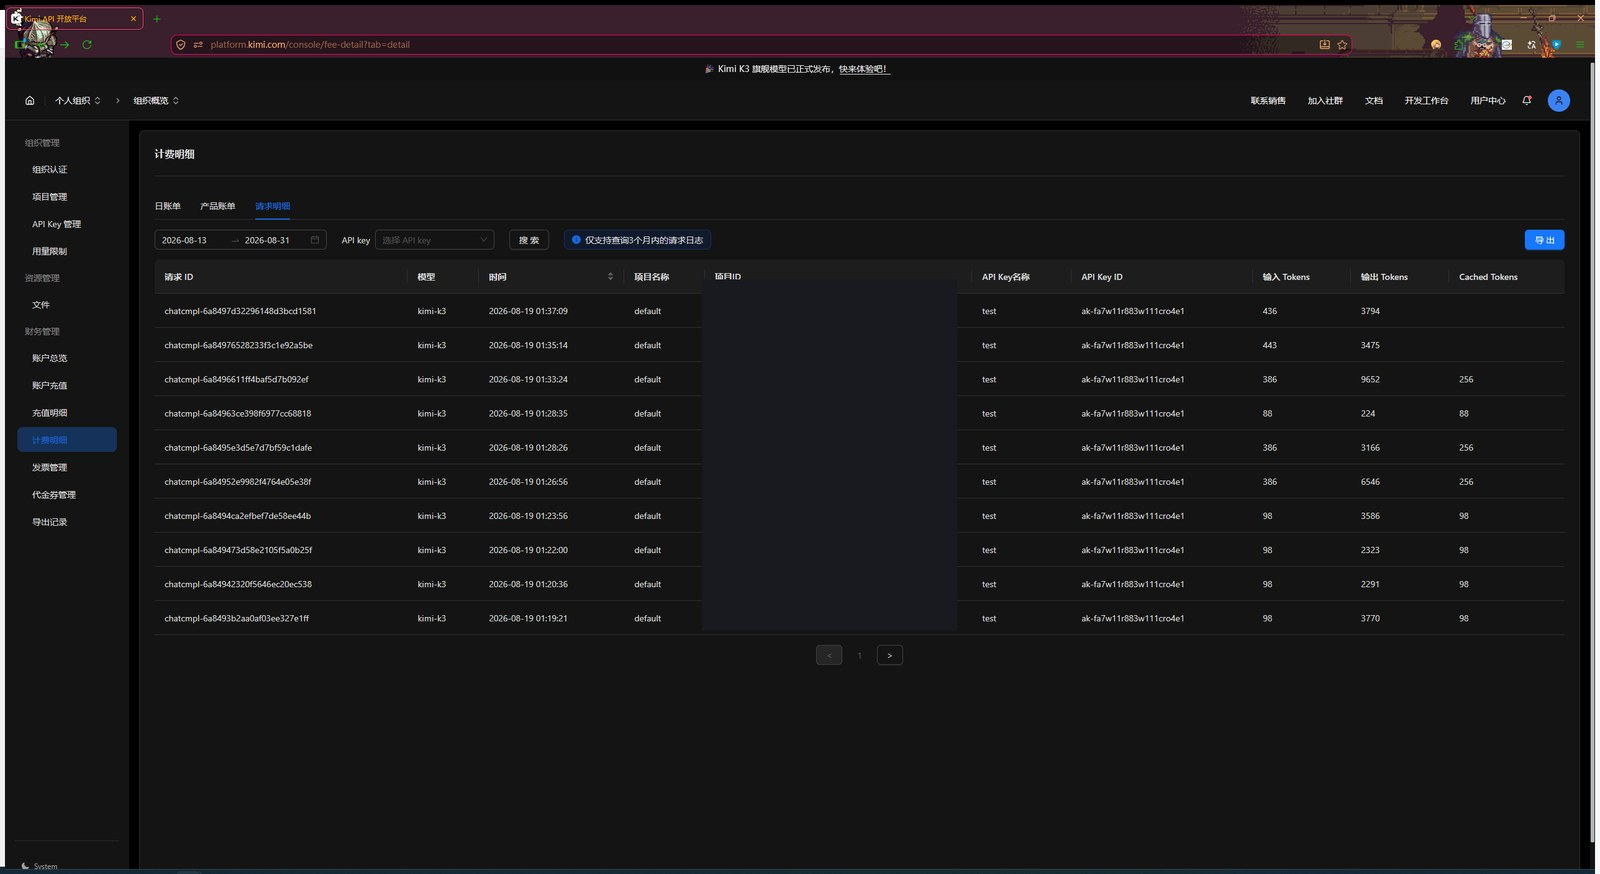
\includegraphics[width=0.92\textwidth]{api_key3.jpg}
\caption{实验 1：Kimi 平台（platform.moonshot.cn）控制台计费明细页面
——kimi-k3 调用记录与输入/输出 Tokens（2026-08-19 多笔调用；API Key
名称与项目 ID 均已脱敏，无 key 明文）。}
\label{fig:ch1_kimi_console}
\end{figure}

\begin{figure}[H]
\centering
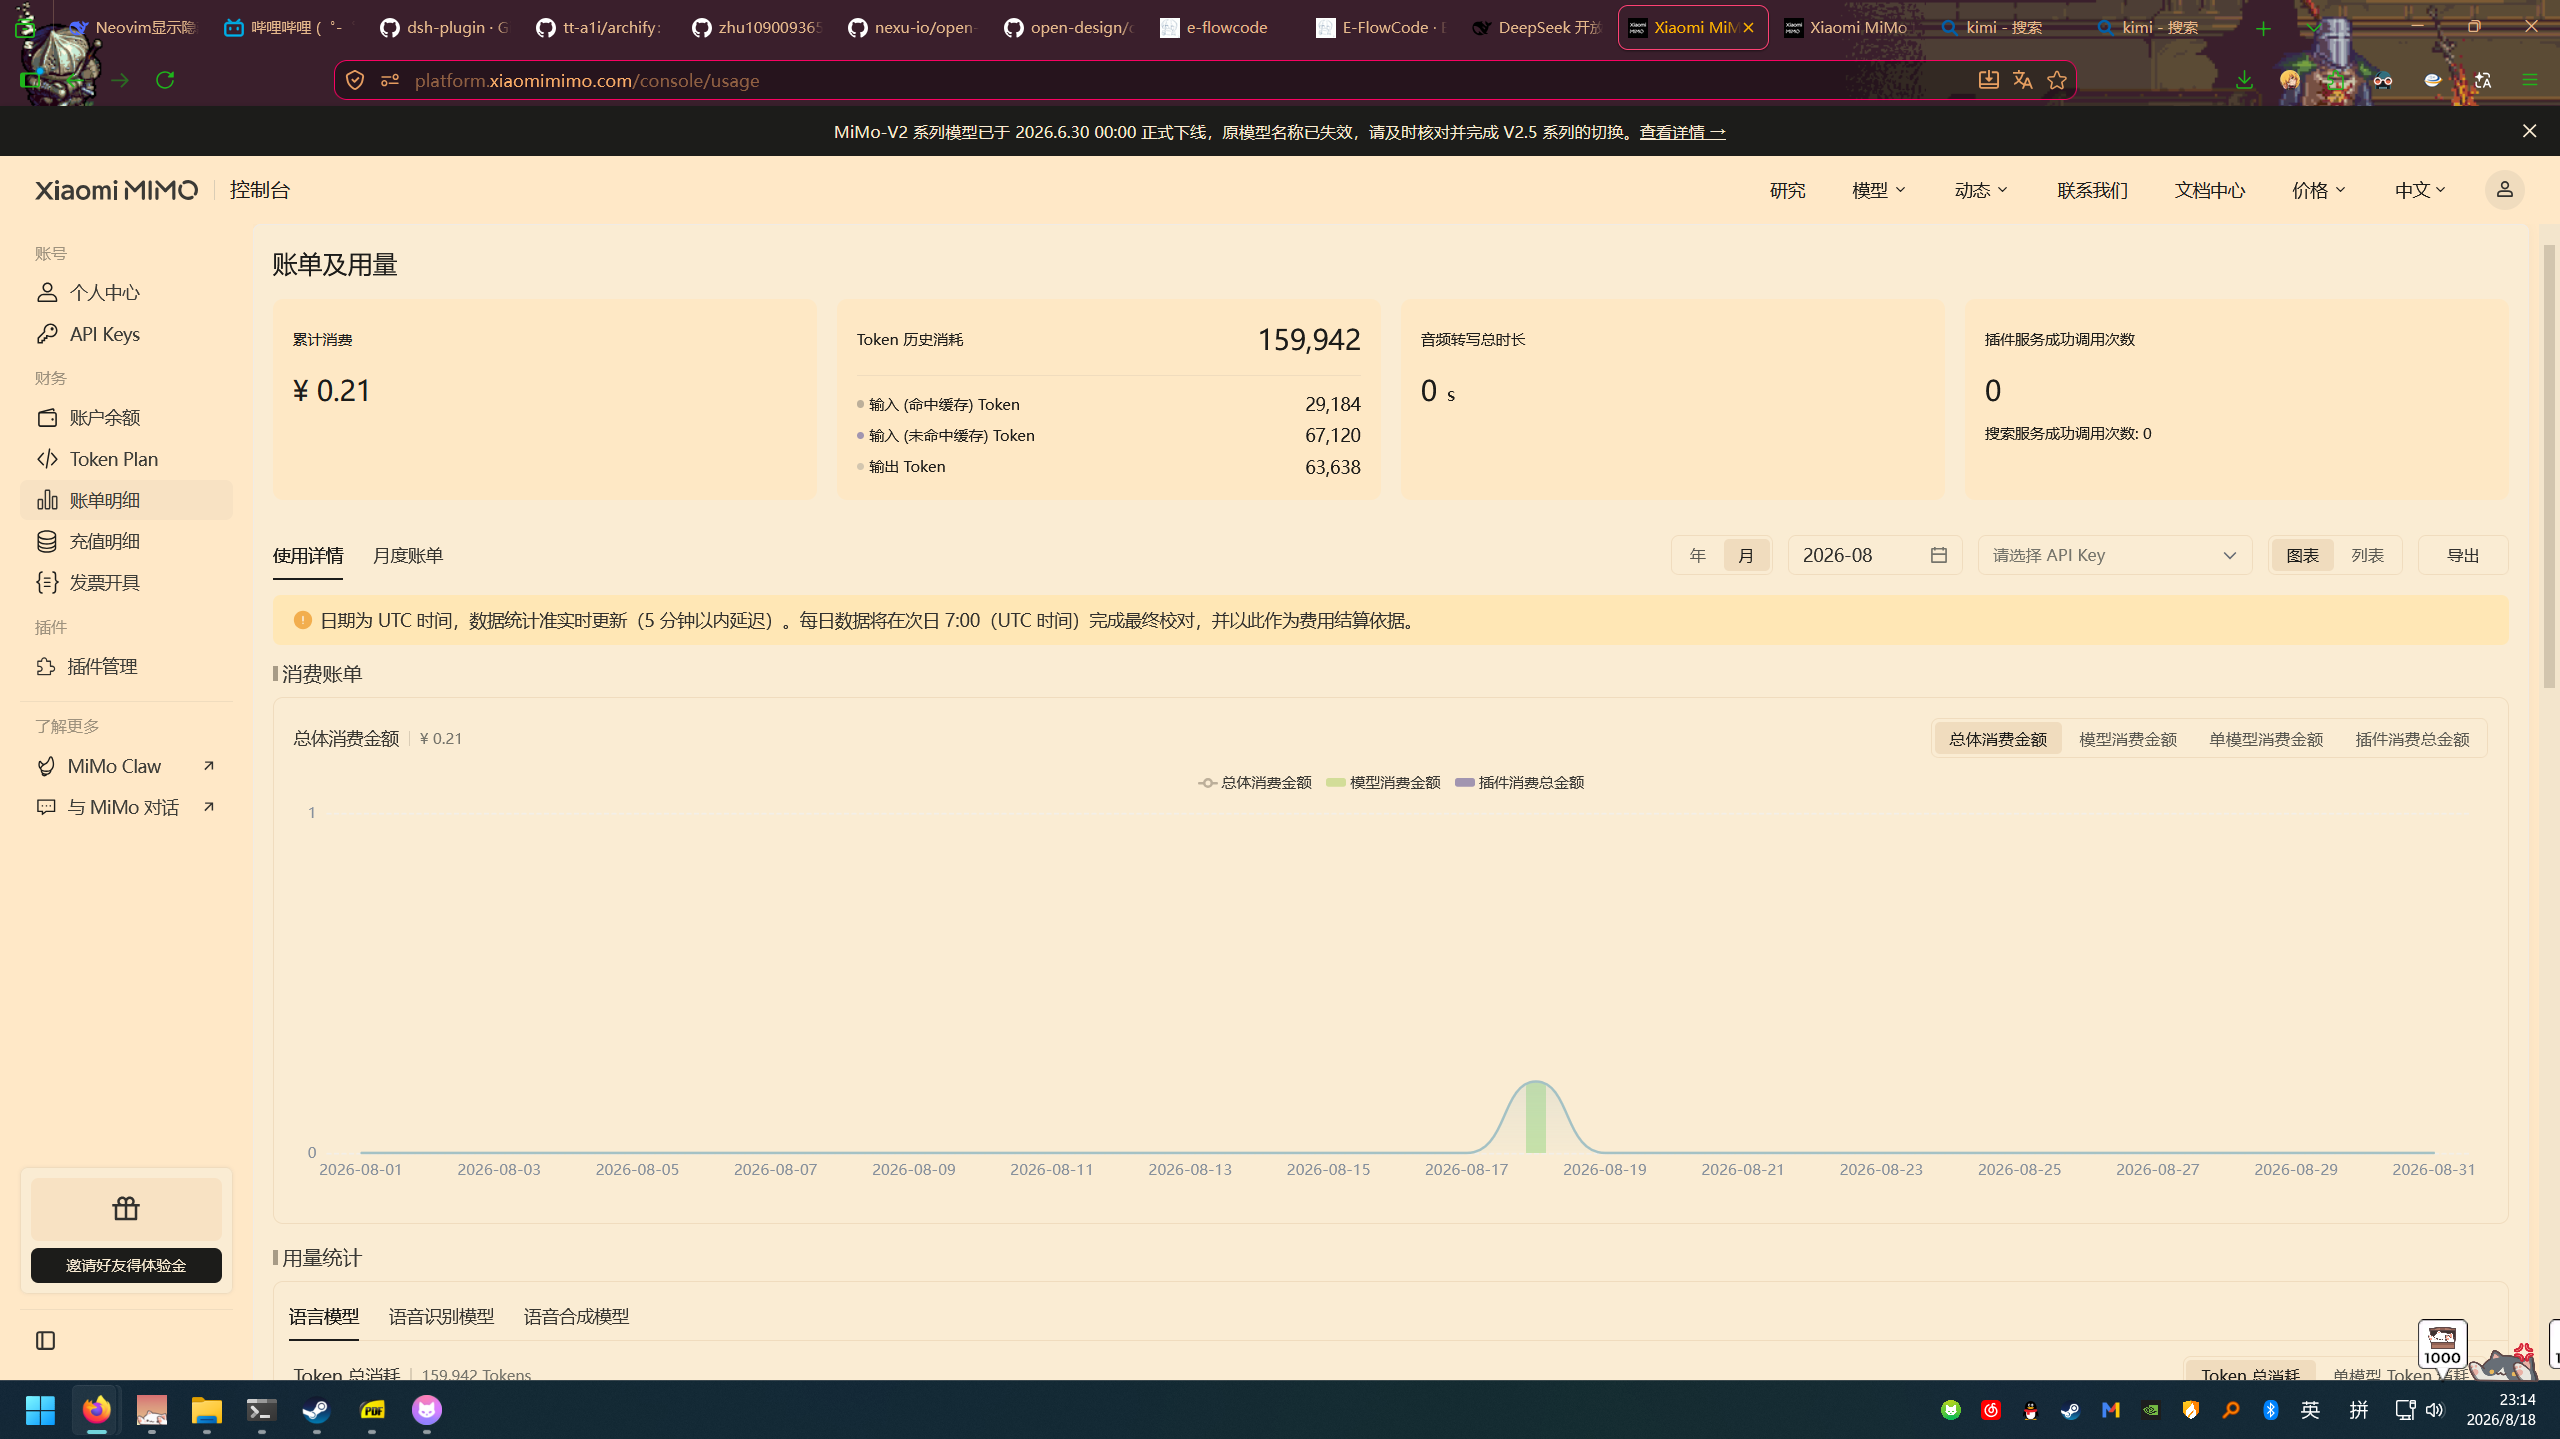
\includegraphics[width=0.92\textwidth]{api_key1.png}
\caption{实验 1：小米 MiMo 平台（platform.xiaomimimo.com）控制台账单及用量页面（累计消费 ¥0.21，无 key 明文）。}
\label{fig:ch1_mimo_console}
\end{figure}

\begin{figure}[H]
\centering
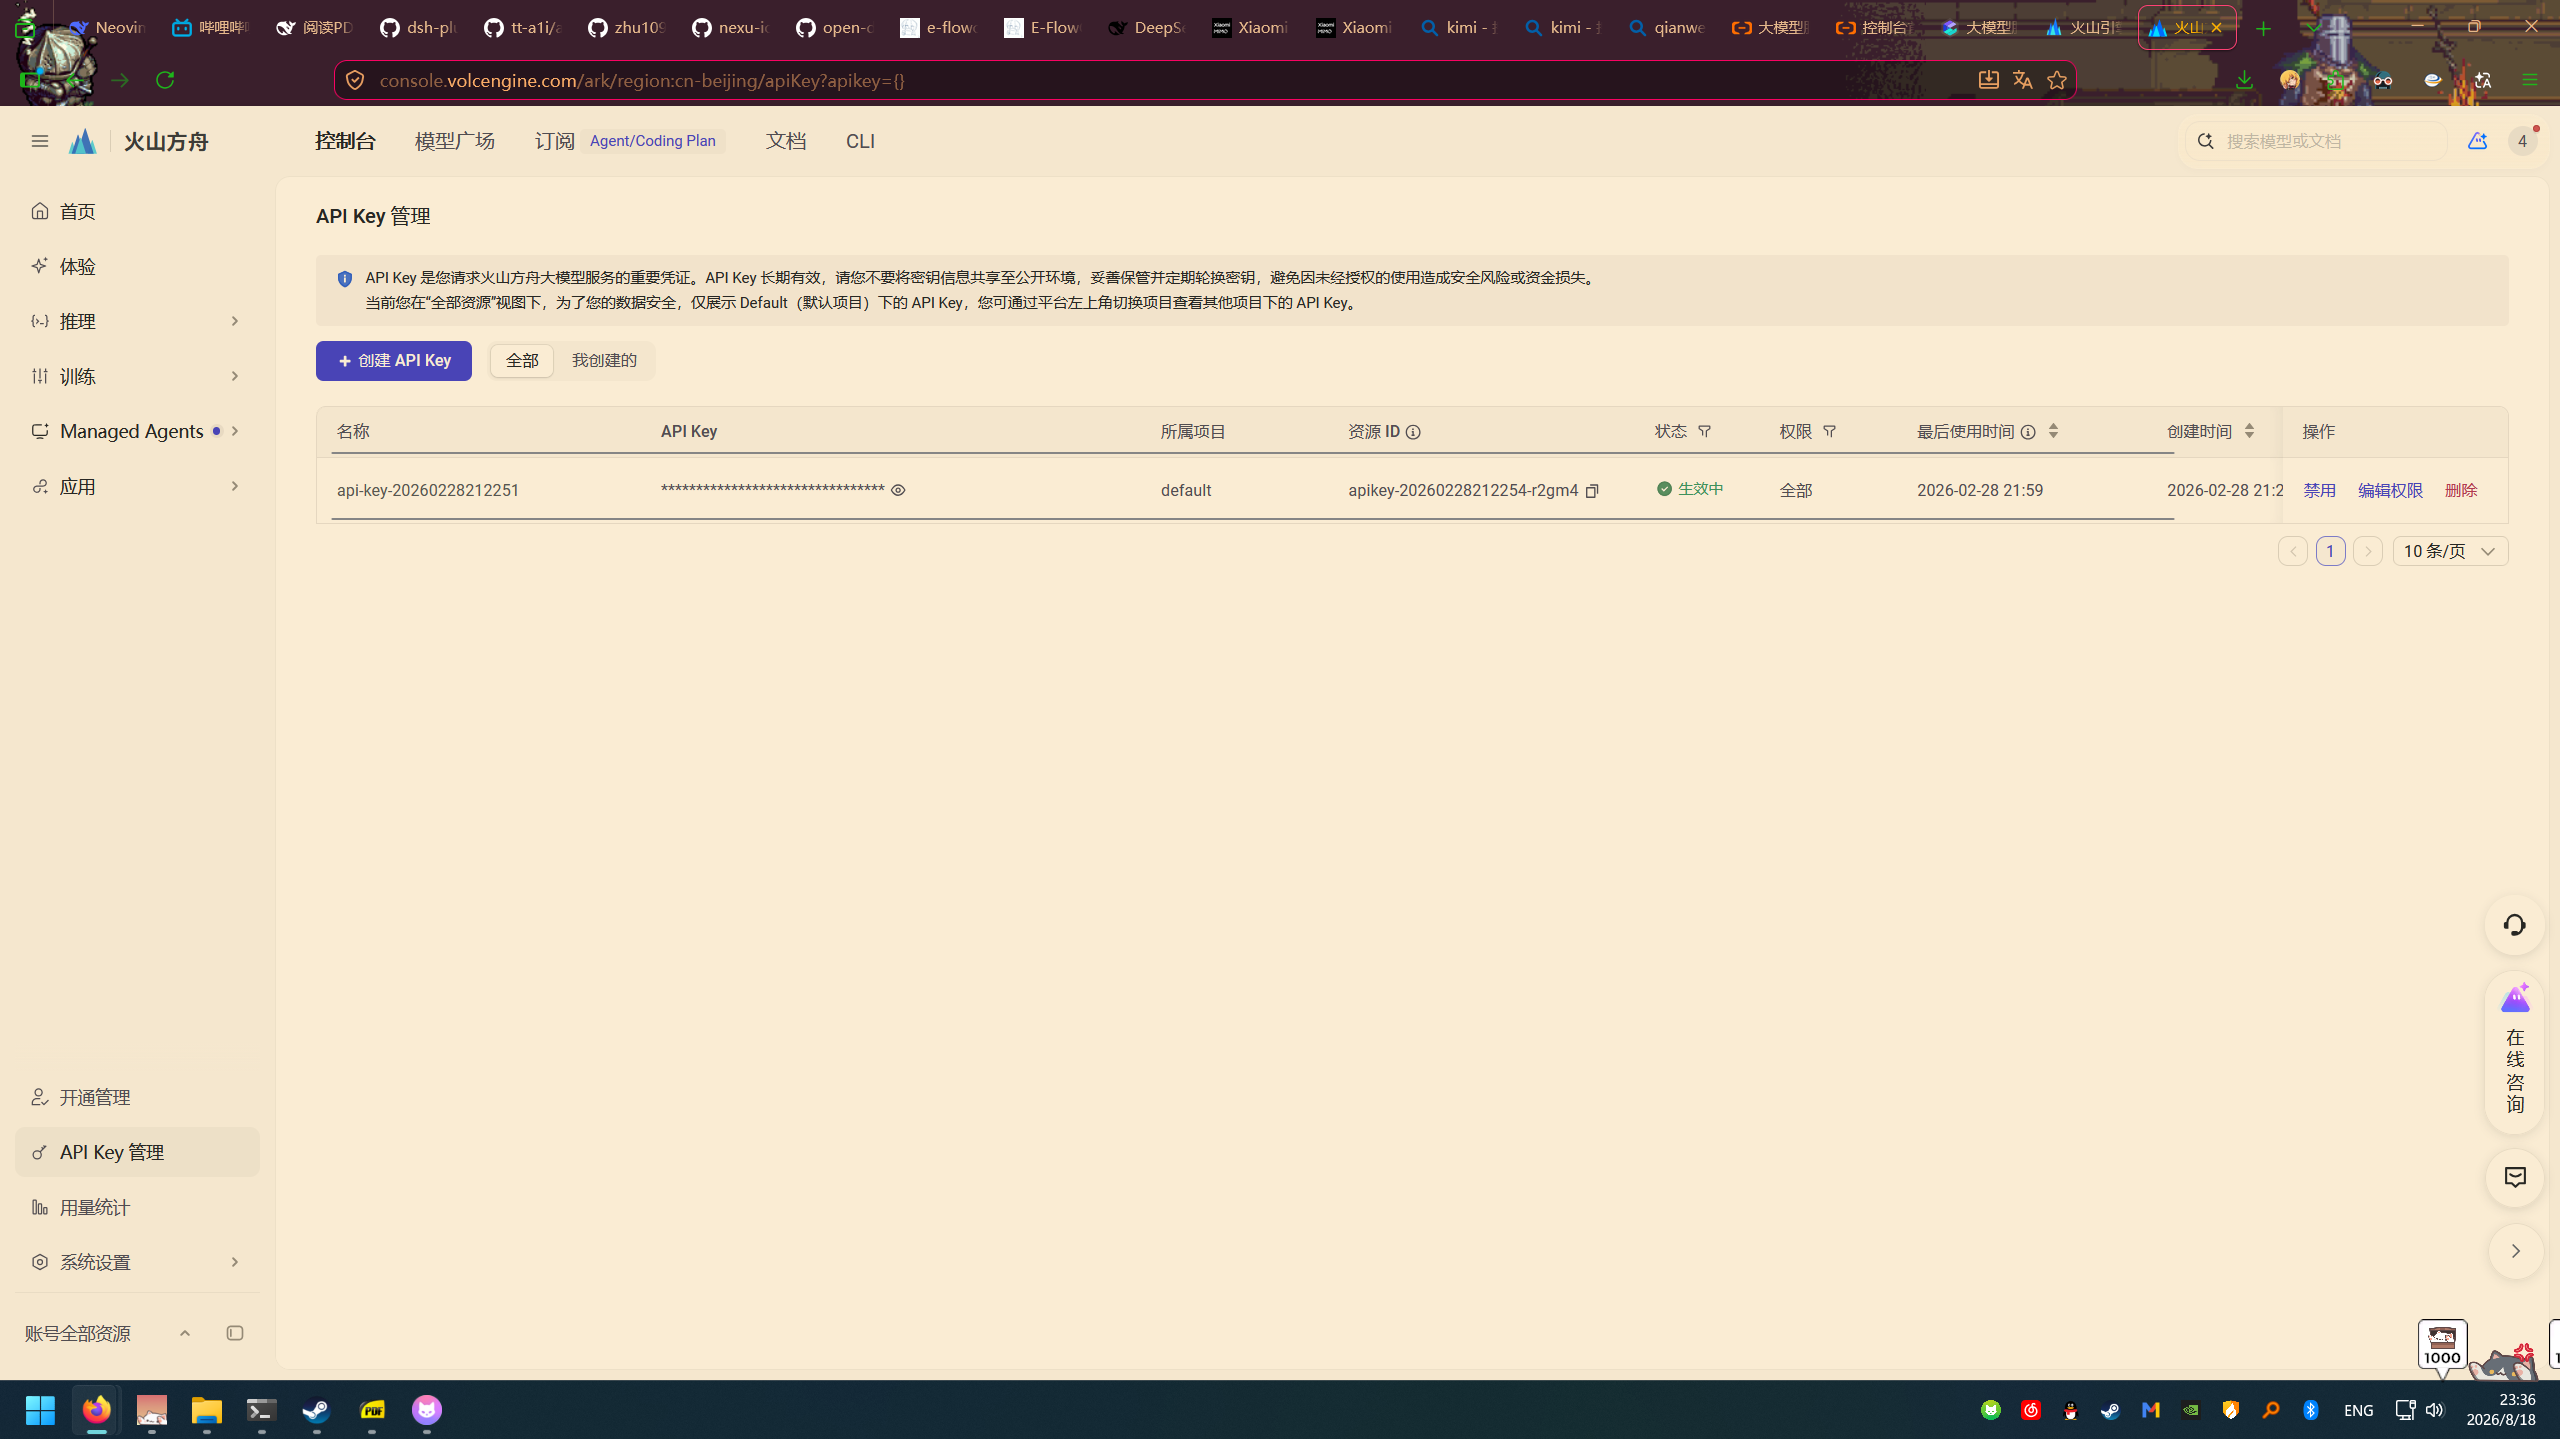
\includegraphics[width=0.92\textwidth]{api_key4.png}
\caption{实验 1：火山方舟（console.volcengine.com/ark）API Key 管理页面（key 以星号遮挡）。}
\label{fig:ch1_ark_console}
\end{figure}

\begin{figure}[H]
\centering
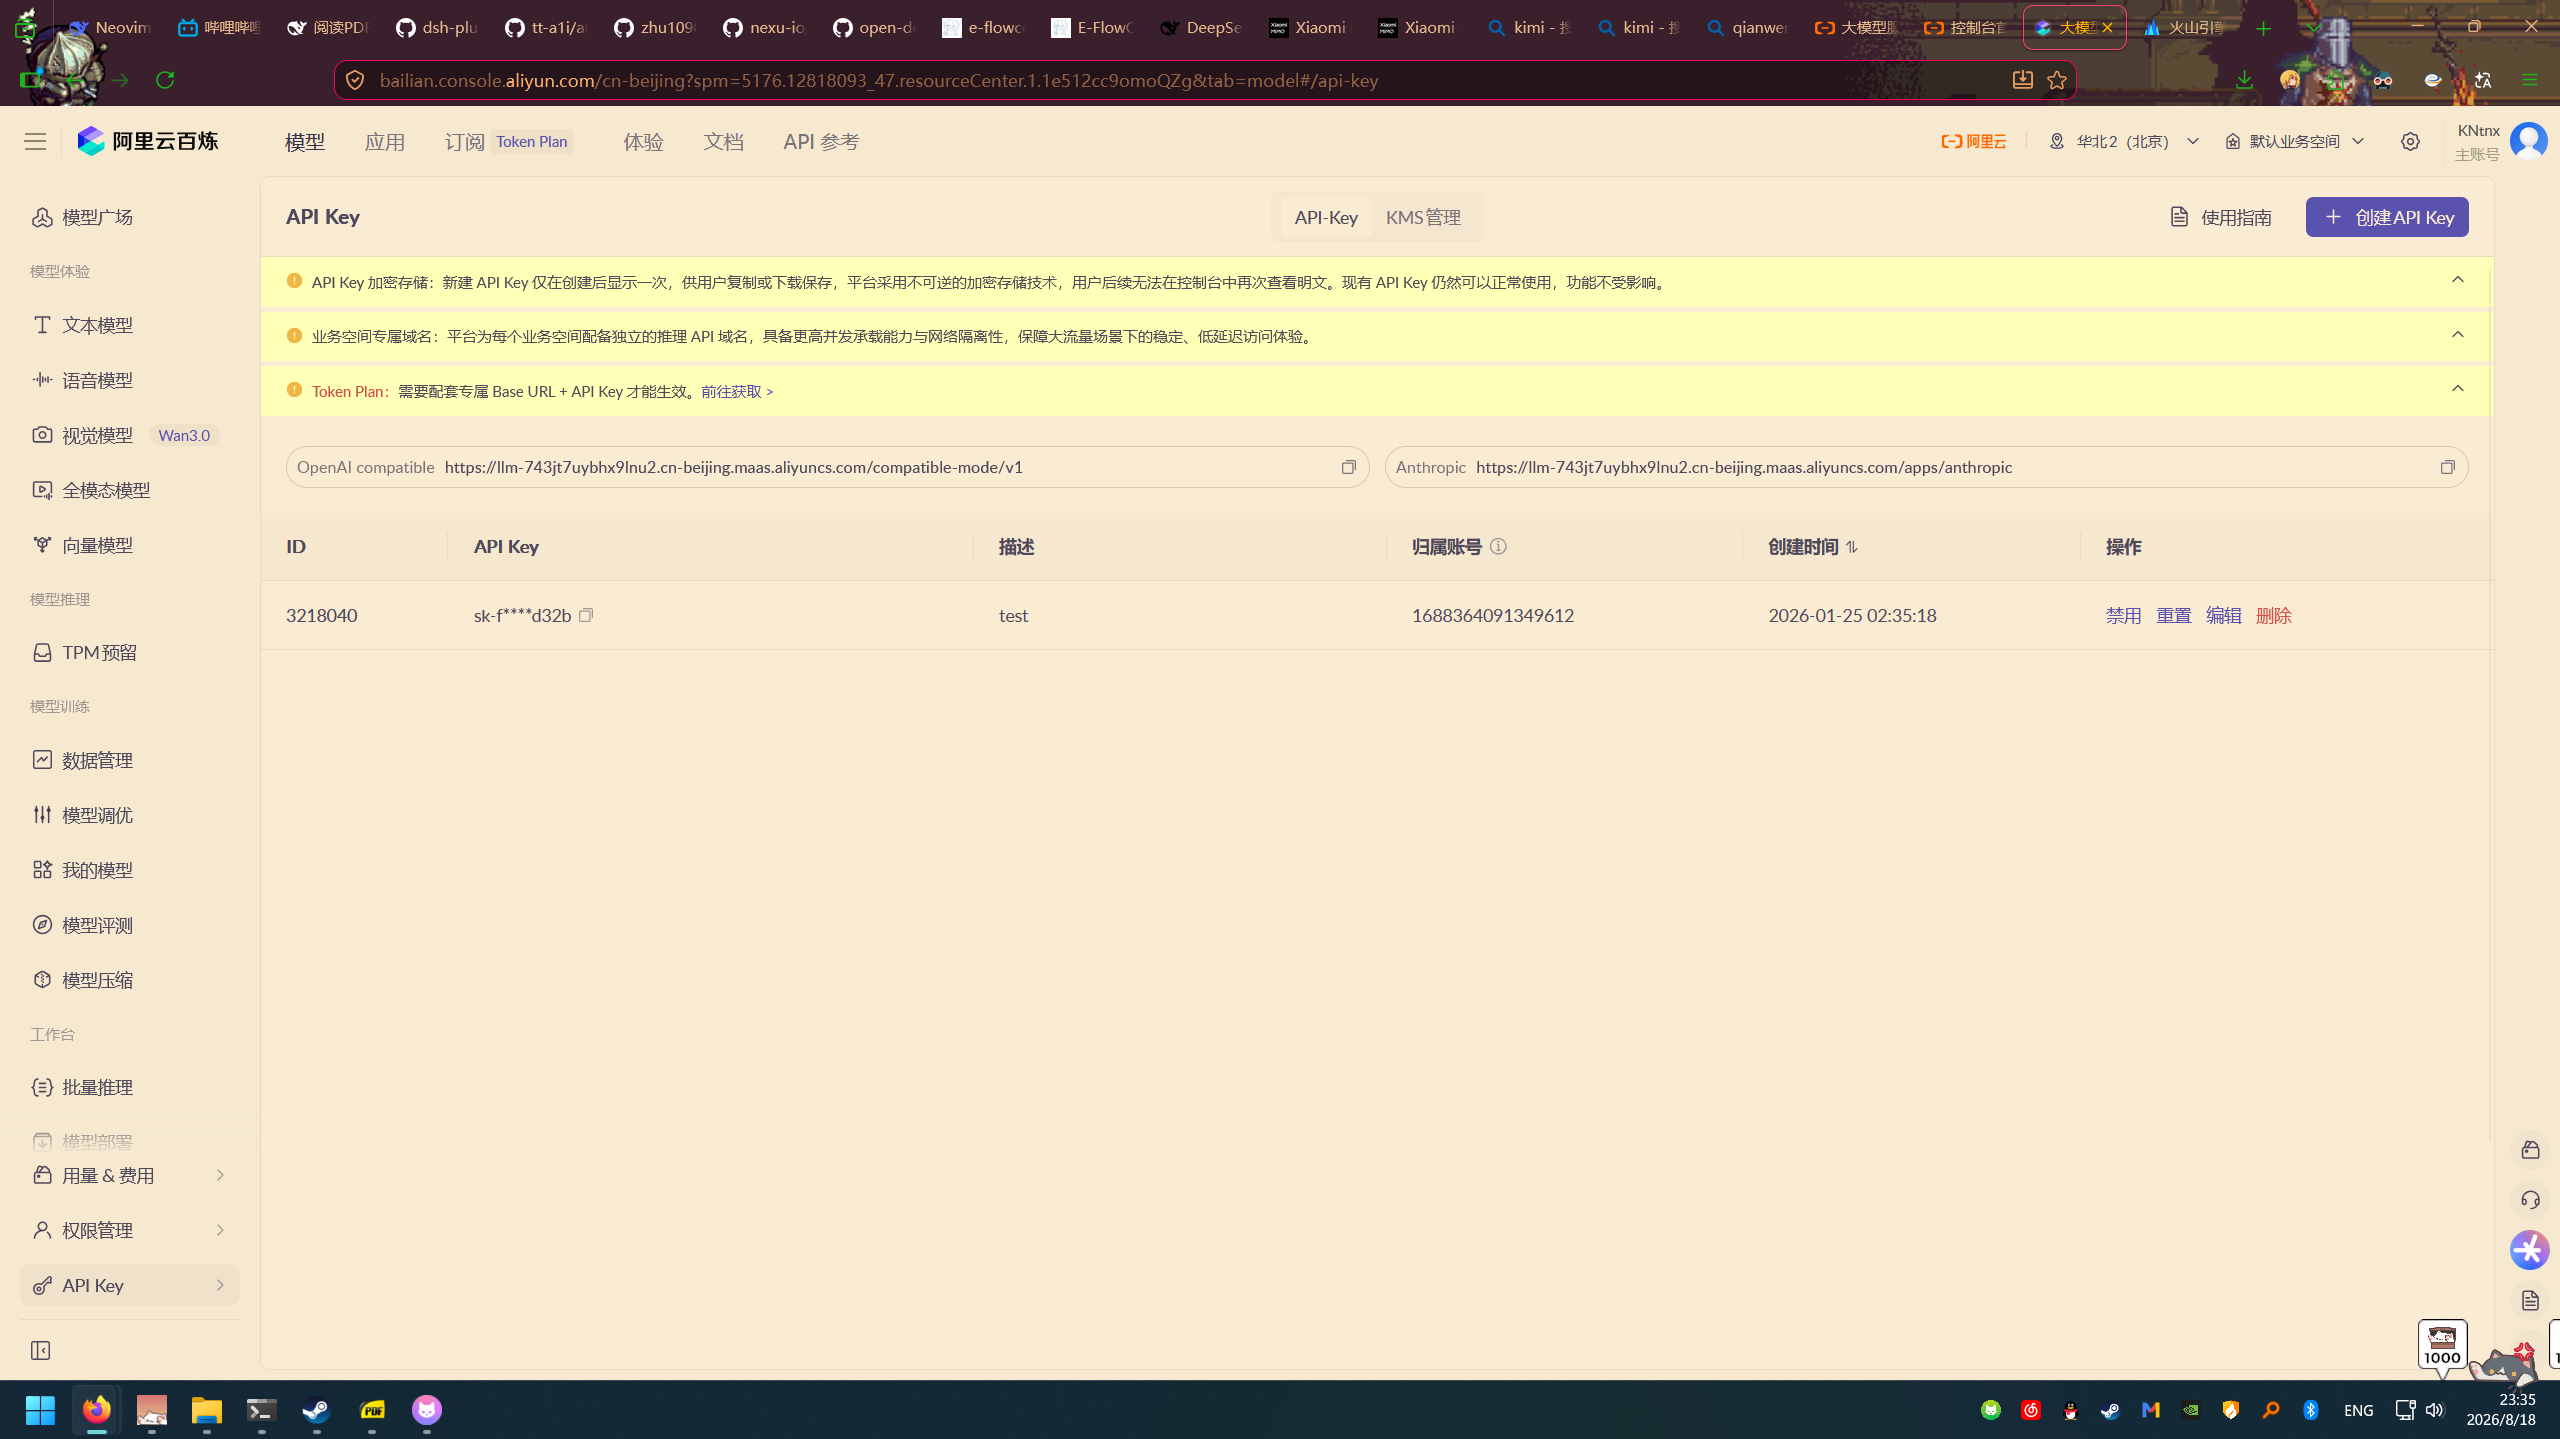
\includegraphics[width=0.92\textwidth]{api_key5.png}
\caption{实验 1：阿里云百炼（bailian.console.aliyun.com）API Key 管理页面（key 以 \texttt{sk-****d32b} 形式部分显示）。}
\label{fig:ch1_qwen_console}
\end{figure}

\begin{figure}[H]
\centering
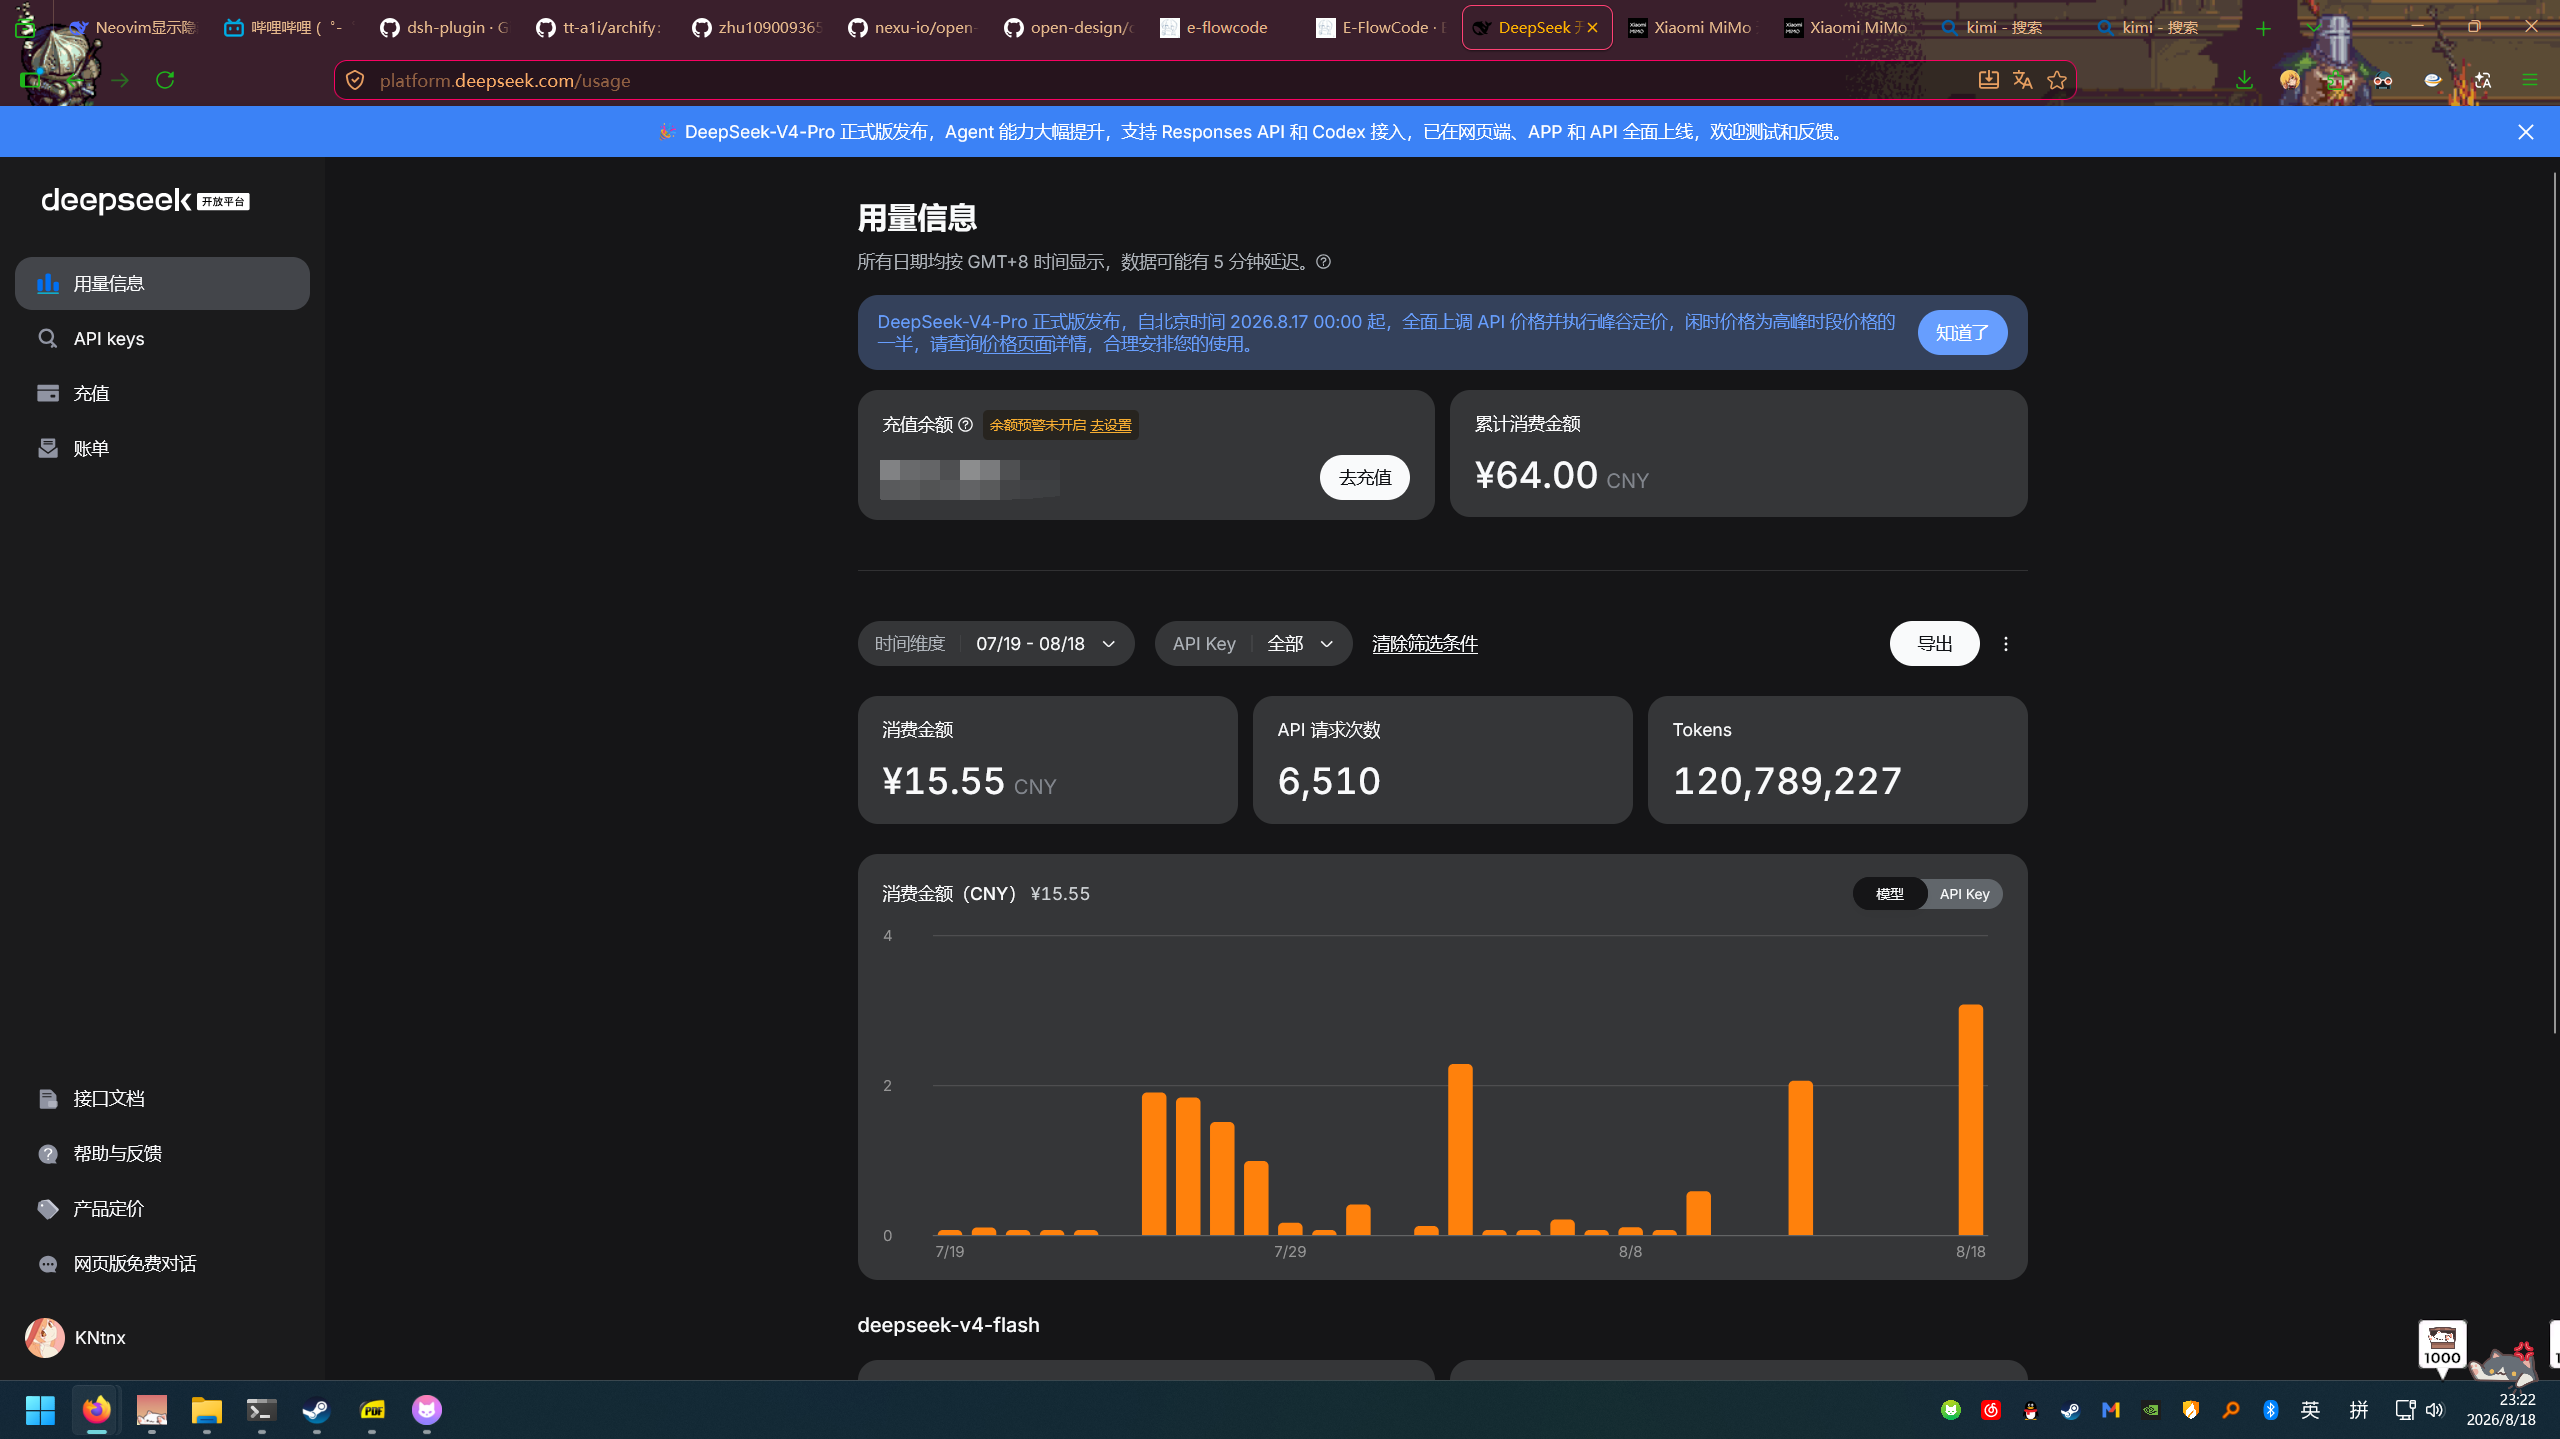
\includegraphics[width=0.92\textwidth]{api_key2.png}
\caption{实验 1：DeepSeek 开放平台（platform.deepseek.com）控制台用量信息页面（充值余额已遮挡；累计消费为账户历史统计，无 key 明文）。}
\label{fig:ch1_ds_console}
\end{figure}

\begin{figure}[H]
\centering
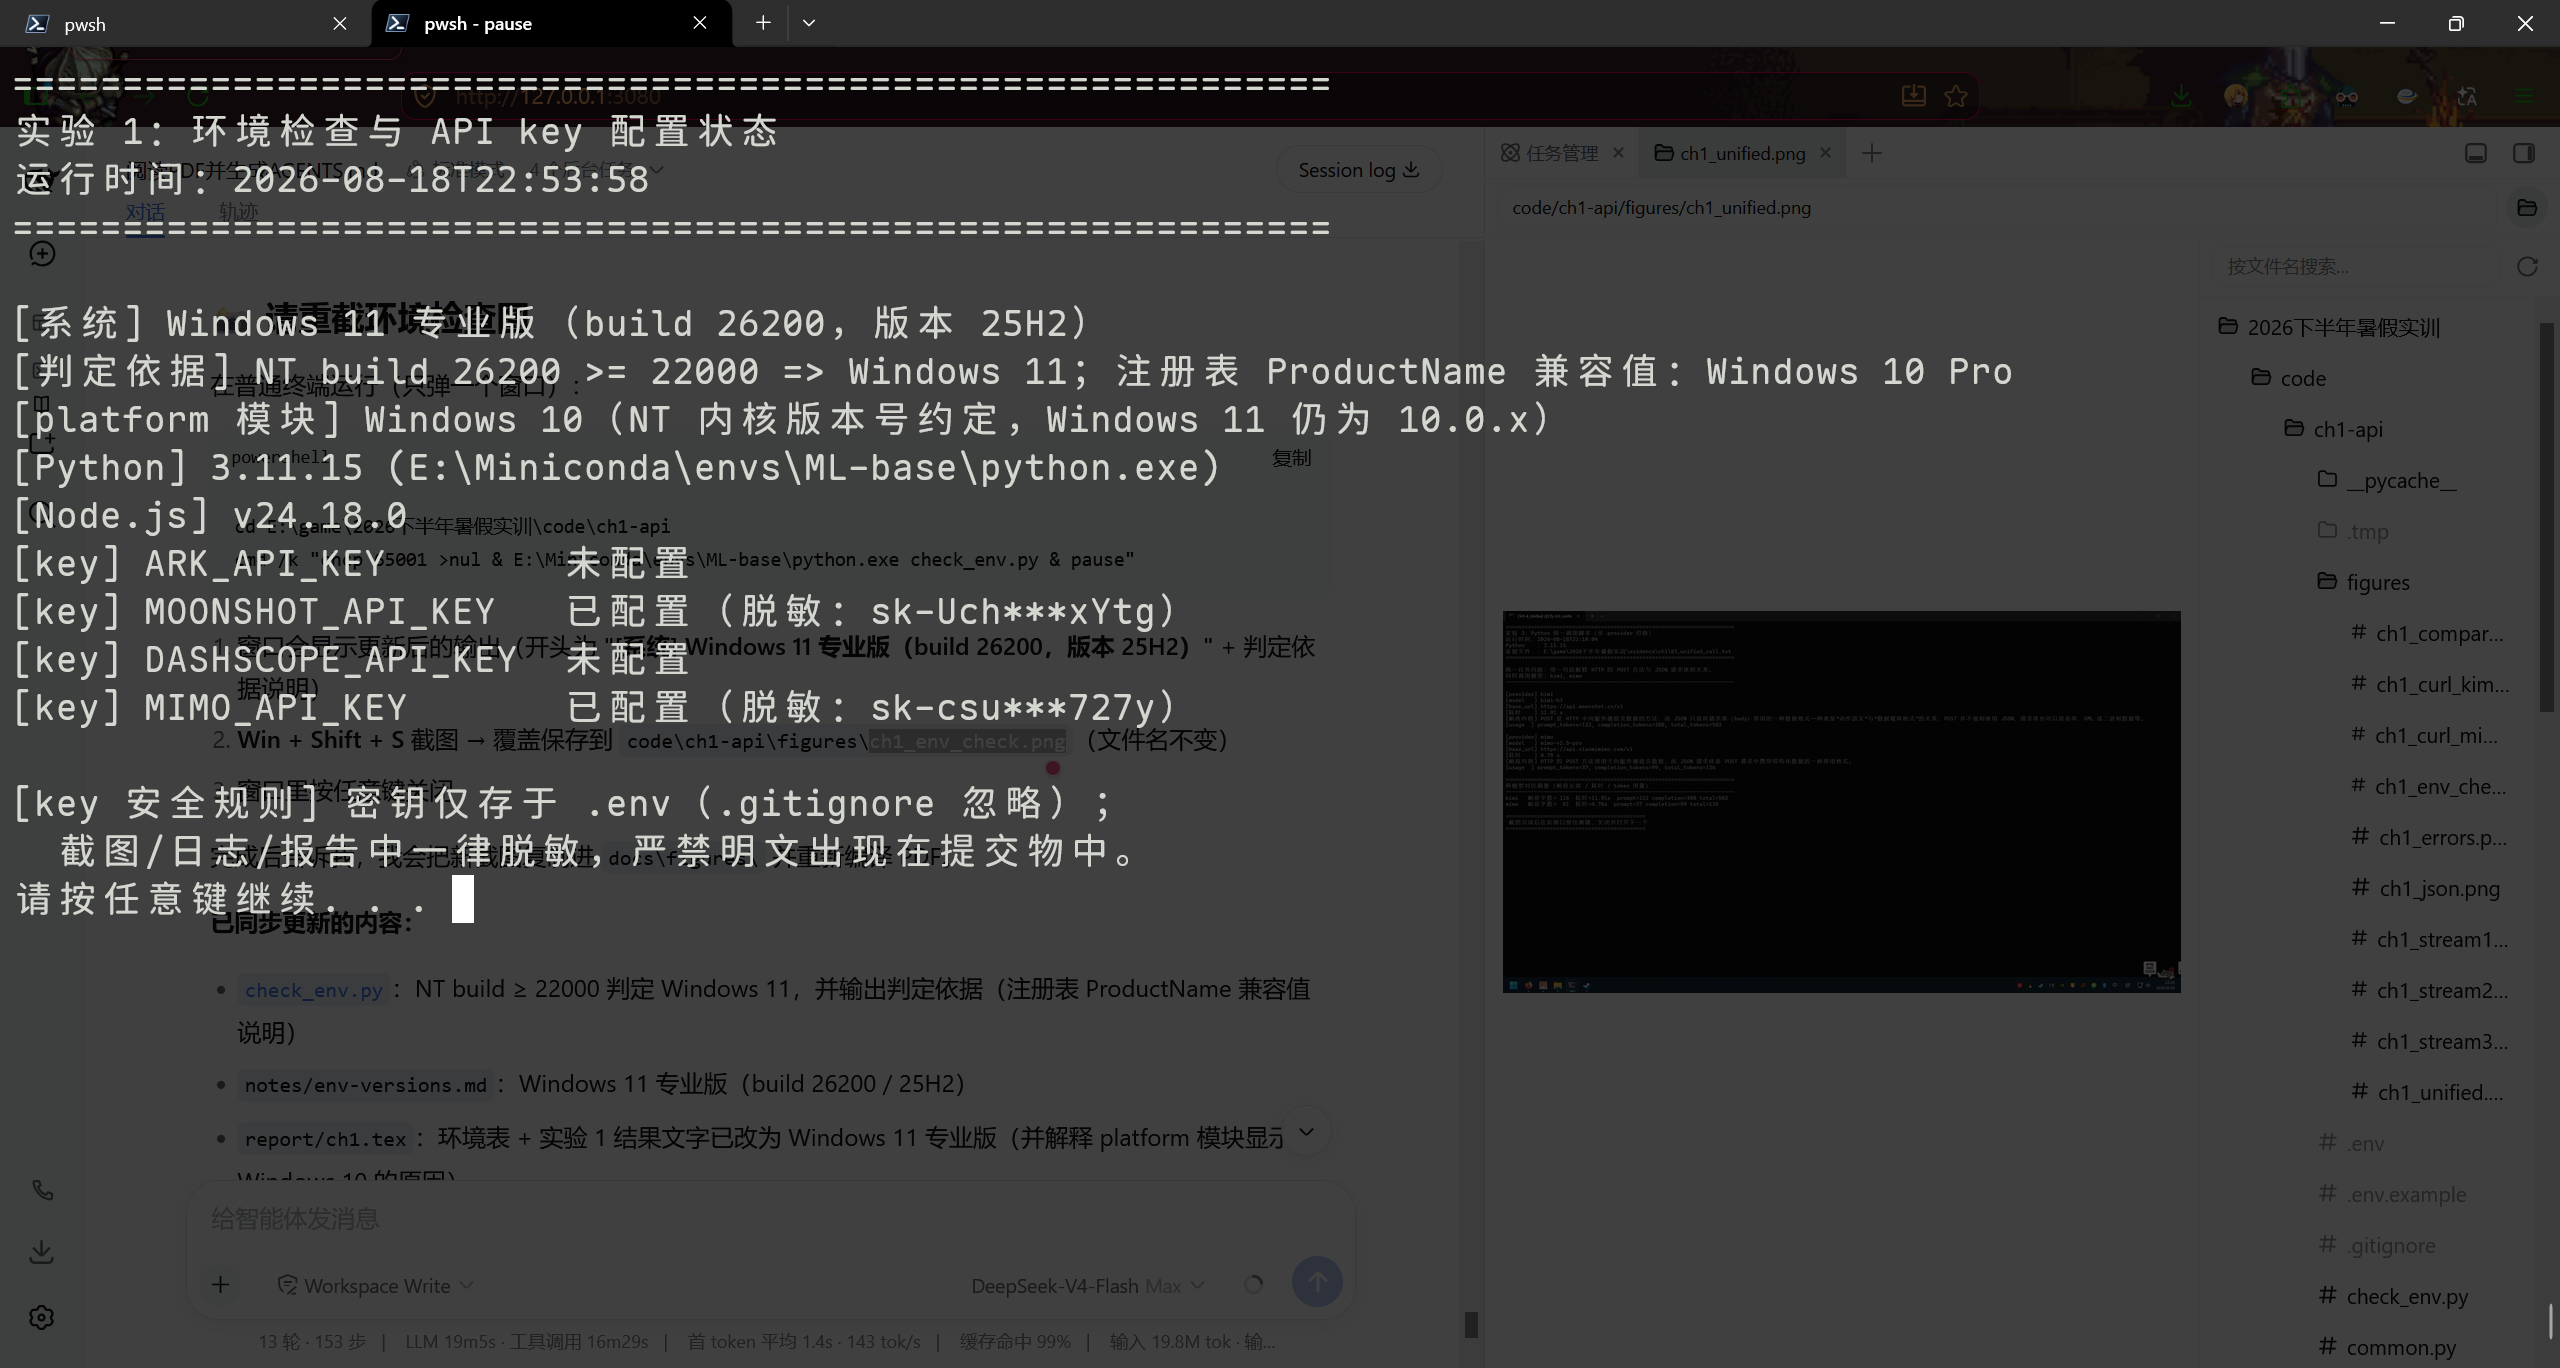
\includegraphics[width=0.92\textwidth]{ch1_env_check.png}
\caption{实验 1：环境检查与 API key 配置状态的真实运行窗口（key 已脱敏显示）。}
\label{fig:ch1_env}
\end{figure}

\subsubsection{实验 2 结果：curl 调用（Kimi 与 MiMo）}

两个 provider 的 \texttt{POST /chat/completions} 均返回 HTTP 200。首次实验使用
\texttt{max\_tokens=150}，出现了一个值得记录的现象：由于 kimi-k3 与 mimo-v2.5-pro
都是默认开启思考模式的推理模型，\texttt{max\_tokens} 预算被推理 token
（reasoning tokens）大量占用，导致正文被截断，\texttt{finish\_reason} 为
\texttt{length}。以 Kimi 为例（截断版响应）：

\begin{verbatim}
{"id":"chatcmpl-6a84574c699481545f155cb3",
 "object":"chat.completion","model":"kimi-k3",
 "choices":[{"index":0,"message":{
   "role":"assistant","content":"",    <- 正文为空！
   "reasoning_content":"The user is asking in
     Chinese to introduce ..."},
   "finish_reason":"length"}],
 "usage":{"prompt_tokens":100,
          "completion_tokens":150,
          "total_tokens":250,
          "completion_tokens_details":{
            "reasoning_tokens":147}}}
\end{verbatim}

150 个 completion token 中有 147 个是推理 token，正文完全没有输出。
将 \texttt{max\_tokens} 提高到 1000 后两个模型都返回完整正文
（Kimi：``POST 是 HTTP 中用于向服务器提交数据的请求方法，而 JSON 是 POST
请求体（body）中最常用的数据格式之一\ldots''；MiMo：``POST 方法负责向服务器
提交数据，而 JSON 请求体是承载这些数据的常用格式——两者是'信封'与'信纸'的
关系''）。真实运行窗口见图~\ref{fig:ch1_curl_kimi} 与
图~\ref{fig:ch1_curl_mimo}，完整响应另见
\texttt{evidence/ch1/02\_curl\_kimi\_full.txt} 与 \texttt{02\_curl\_mimo\_full.txt}。

\begin{figure}[H]
\centering
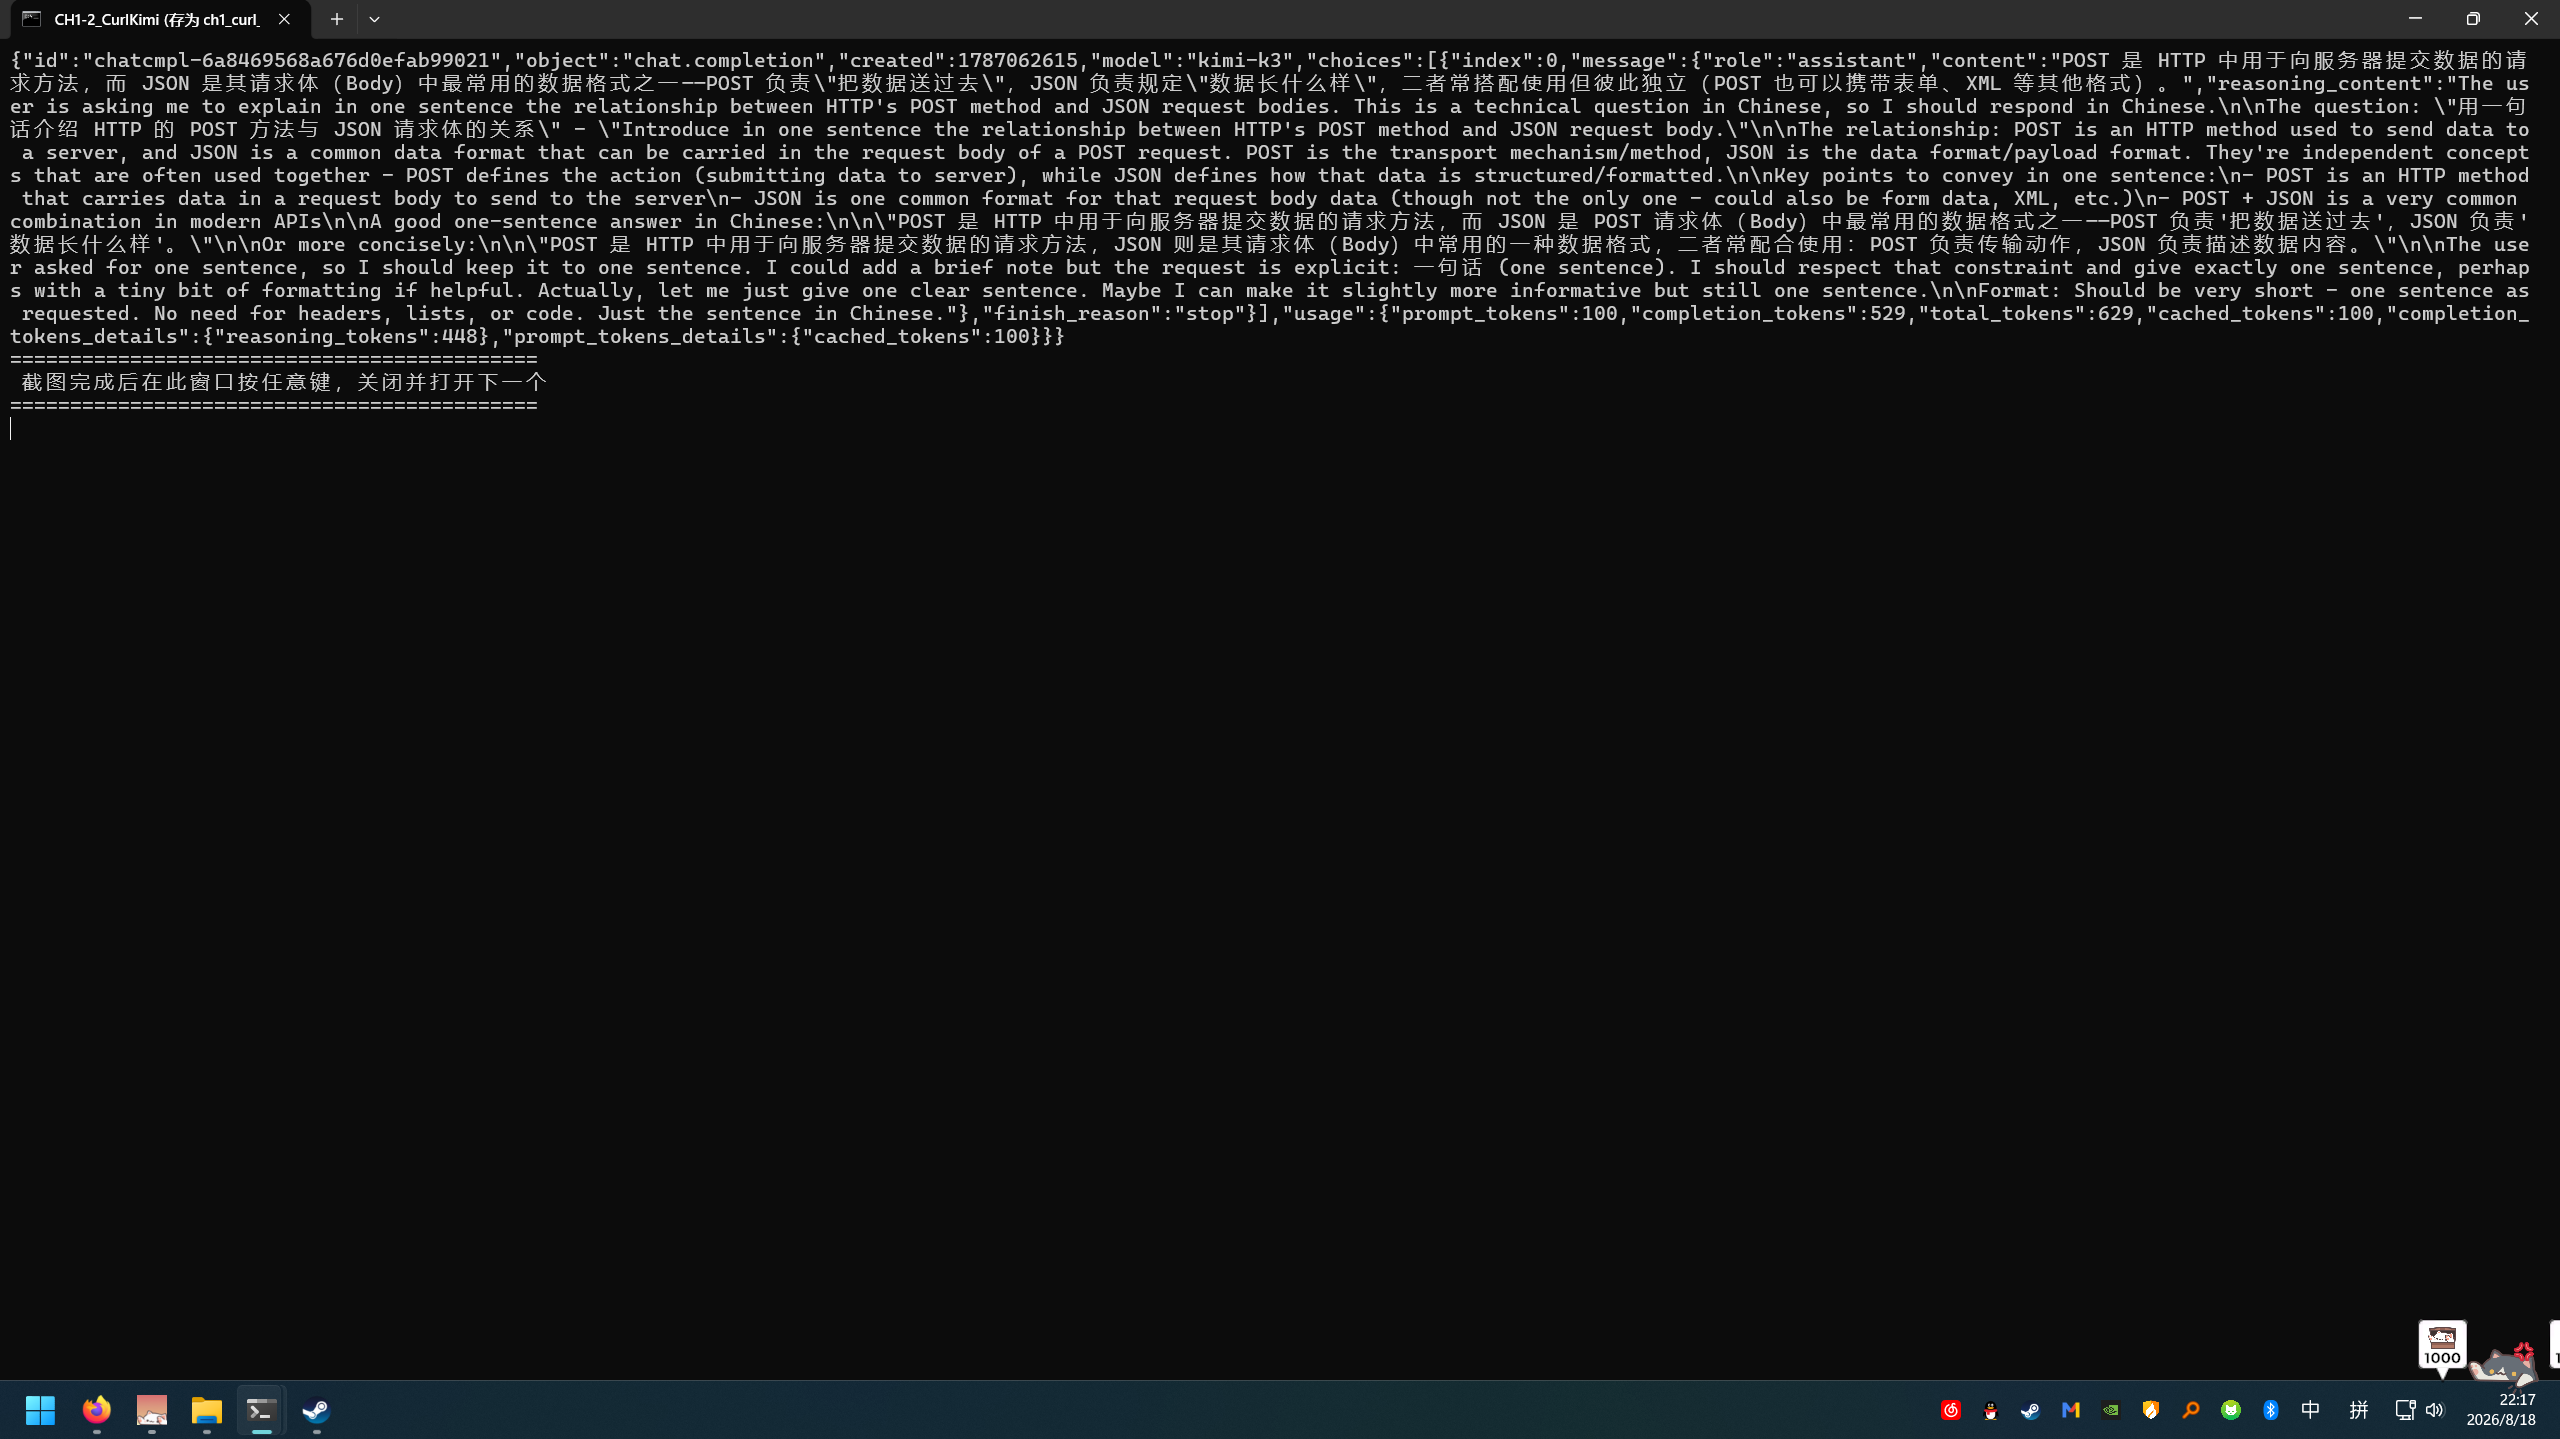
\includegraphics[width=0.92\textwidth]{ch1_curl_kimi.png}
\caption{实验 2：curl 调用 Kimi（kimi-k3）的真实运行窗口，返回完整响应与 usage。}
\label{fig:ch1_curl_kimi}
\end{figure}

\begin{figure}[H]
\centering
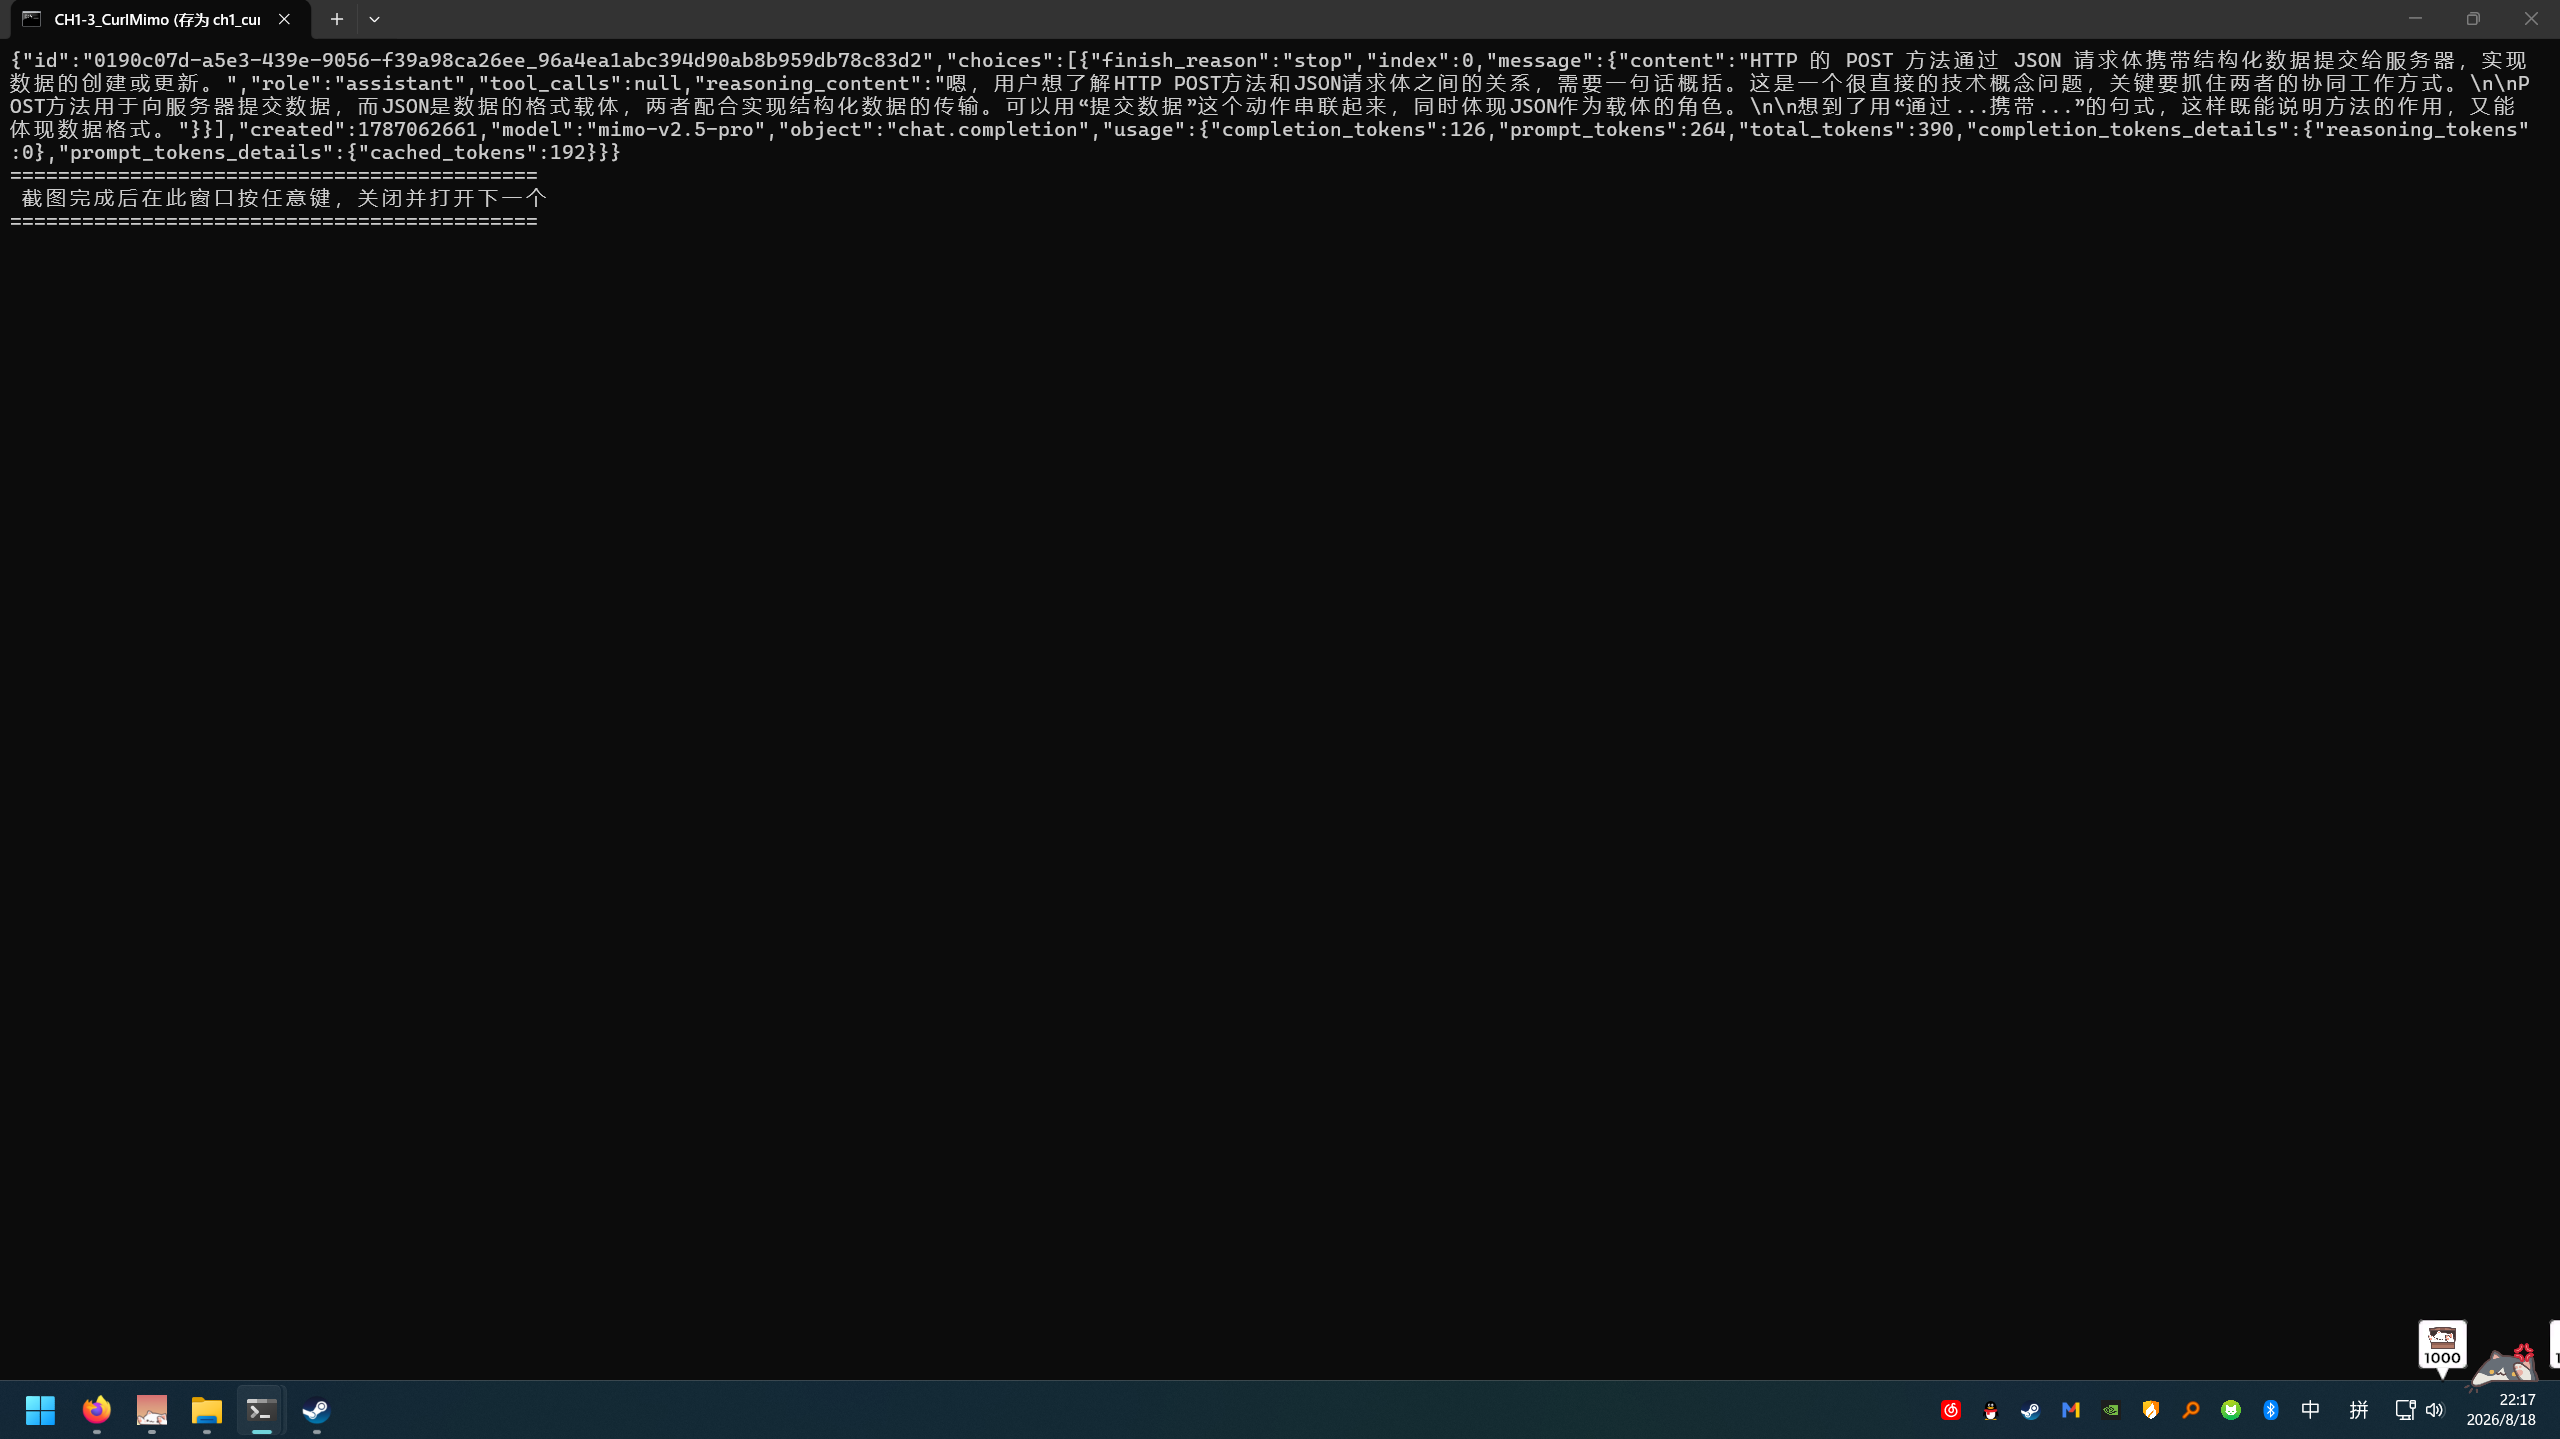
\includegraphics[width=0.92\textwidth]{ch1_curl_mimo.png}
\caption{实验 2：curl 调用小米 MiMo（mimo-v2.5-pro）的真实运行窗口。}
\label{fig:ch1_curl_mimo}
\end{figure}

\subsubsection{实验 3 结果：Python 统一调用}

同一问题（``用一句话解释 HTTP 的 POST 方法与 JSON 请求体的关系''）同时调用
kimi-k3 与 mimo-v2.5-pro，结果见表~\ref{tab:ch1_unified}，完整输出见
\nolinkurl{evidence/ch1/03_unified_call.txt}。

\begin{table}[H]
\centering
\caption{统一调用结果对比（同一问题）}
\label{tab:ch1_unified}
\begin{tabular}{lcc}
\toprule
\textbf{指标} & \textbf{kimi-k3} & \textbf{mimo-v2.5-pro} \\
\midrule
总耗时 (s) & 14.12 & 5.15 \\
响应字数 & 138 & 61 \\
prompt\_tokens & 122 & 37 \\
completion\_tokens & 280 & 130 \\
total\_tokens & 402 & 167 \\
\bottomrule
\end{tabular}
\end{table}

两个模型都给出了准确回答。Kimi 的回答更详细（补充了
\texttt{Content-Type: application/json} 的语义），MiMo 的回答更简洁；
MiMo 的 prompt\_tokens 明显更少，与其 tokenizer 分词粒度及提示词缓存
（cached\_tokens）有关。同一份代码只需切换 PROVIDERS 字典即可换平台，
验证了 OpenAI-compatible 的低迁移成本。真实运行窗口见图~\ref{fig:ch1_unified}。

\begin{figure}[H]
\centering
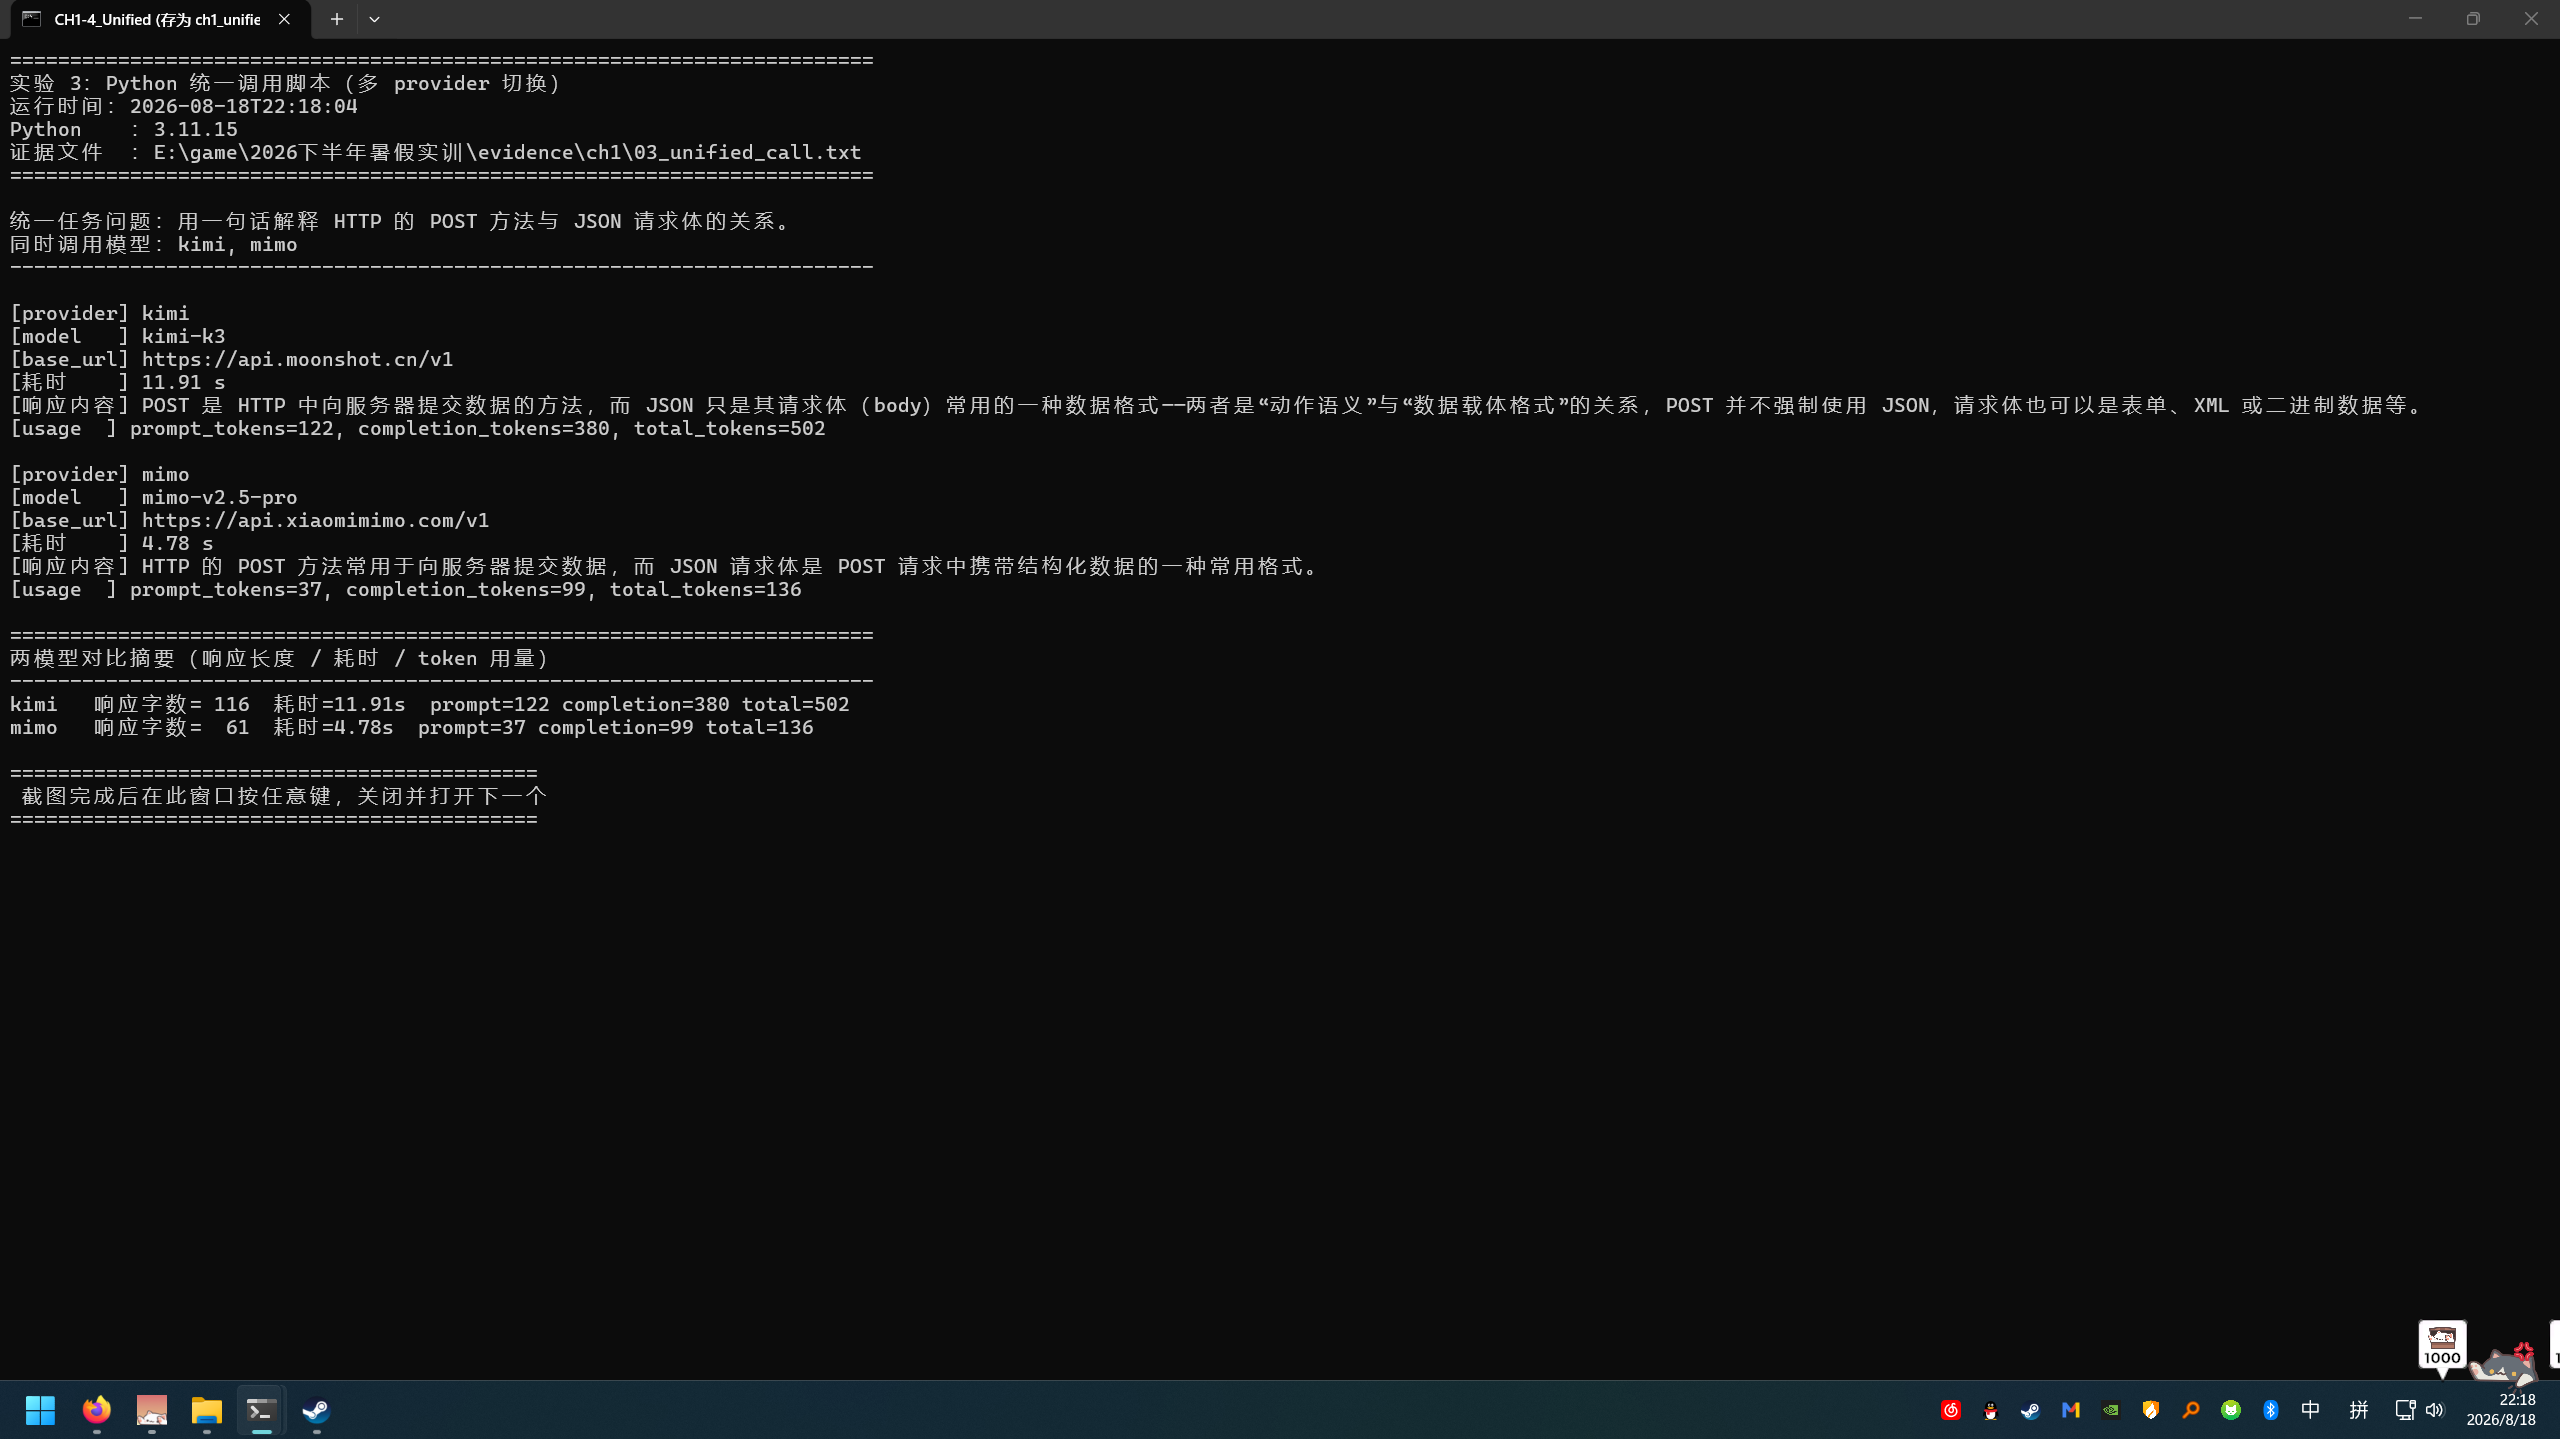
\includegraphics[width=0.92\textwidth]{ch1_unified.png}
\caption{实验 3：统一调用脚本同时调用 kimi-k3 与 mimo-v2.5-pro 的真实运行窗口，含响应内容、usage 与对比摘要。}
\label{fig:ch1_unified}
\end{figure}

\subsubsection{实验 4 结果：流式输出}

以 kimi-k3 为例，一次流式调用共收到 375 个 chunk。前 160 余个 chunk 的
\texttt{delta.content} 为 \texttt{None}（模型处于推理阶段），之后才逐字输出
正文，最后以 \texttt{finish\_reason=stop} 结束，并通过空 choices 的 chunk
携带 usage。关键 chunk 结构（节选）：

\begin{verbatim}
chunk delta.content=''        <- 首个 chunk（含 role）
chunk delta.content=None      <- 推理阶段：约 160 个 chunk 无正文
...（省略推理 chunk）...
chunk delta.content='流'      <- 正文开始，逐 token 输出
chunk delta.content='式'
chunk delta.content='输出'
...
chunk finish_reason=stop      <- 结束
[usage chunk] {'completion_tokens': 387,
  'prompt_tokens': 119,
  'completion_tokens_details':
    {'reasoning_tokens': 294}}
\end{verbatim}

流式与普通输出的对比见表~\ref{tab:ch1_stream}。流式模式首字节延迟
（TTFT）为 2.68 s，之后内容边生成边到达；普通模式需要等待完整响应
（13.24 s）才能开始渲染。两者的最终内容与 token 用量一致。真实运行窗口
见图~\ref{fig:ch1_stream_chunks}（推理阶段 chunk 与正文 chunk）与
图~\ref{fig:ch1_stream_summary}（流式汇总与普通调用对照）。

对 MiMo 的补充验证（\nolinkurl{test_mimo_stream_usage.py}，证据
\nolinkurl{05c_mimo_stream_usage.txt}）表明：\texttt{mimo-v2.5-pro} 同样
支持 \texttt{stream\_options}（设为 \texttt{include\_usage=True}）参数，
流式末尾返回 usage chunk（45 个 chunk，prompt=265、completion=101，含
\texttt{cached\_tokens=192}）。两个平台的流式 usage 均可获得，区别在于
Kimi 的 usage 含 \texttt{reasoning\_tokens} 明细（推理 token 单独统计），
MiMo 的 usage 结构与模型相关。

\begin{table}[H]
\centering
\caption{流式输出与普通输出对比（kimi-k3）}
\label{tab:ch1_stream}
\begin{tabular}{lcc}
\toprule
\textbf{指标} & \textbf{流式 (stream=True)} & \textbf{普通} \\
\midrule
首字节延迟 TTFT (s) & 2.68 & 13.24（即总耗时） \\
总耗时 (s) & 14.07 & 13.24 \\
chunk 数 & 375 & 1 \\
usage（prompt/completion/total） & 119/387/506 & 一致 \\
\bottomrule
\end{tabular}
\end{table}

\begin{figure}[H]
\centering
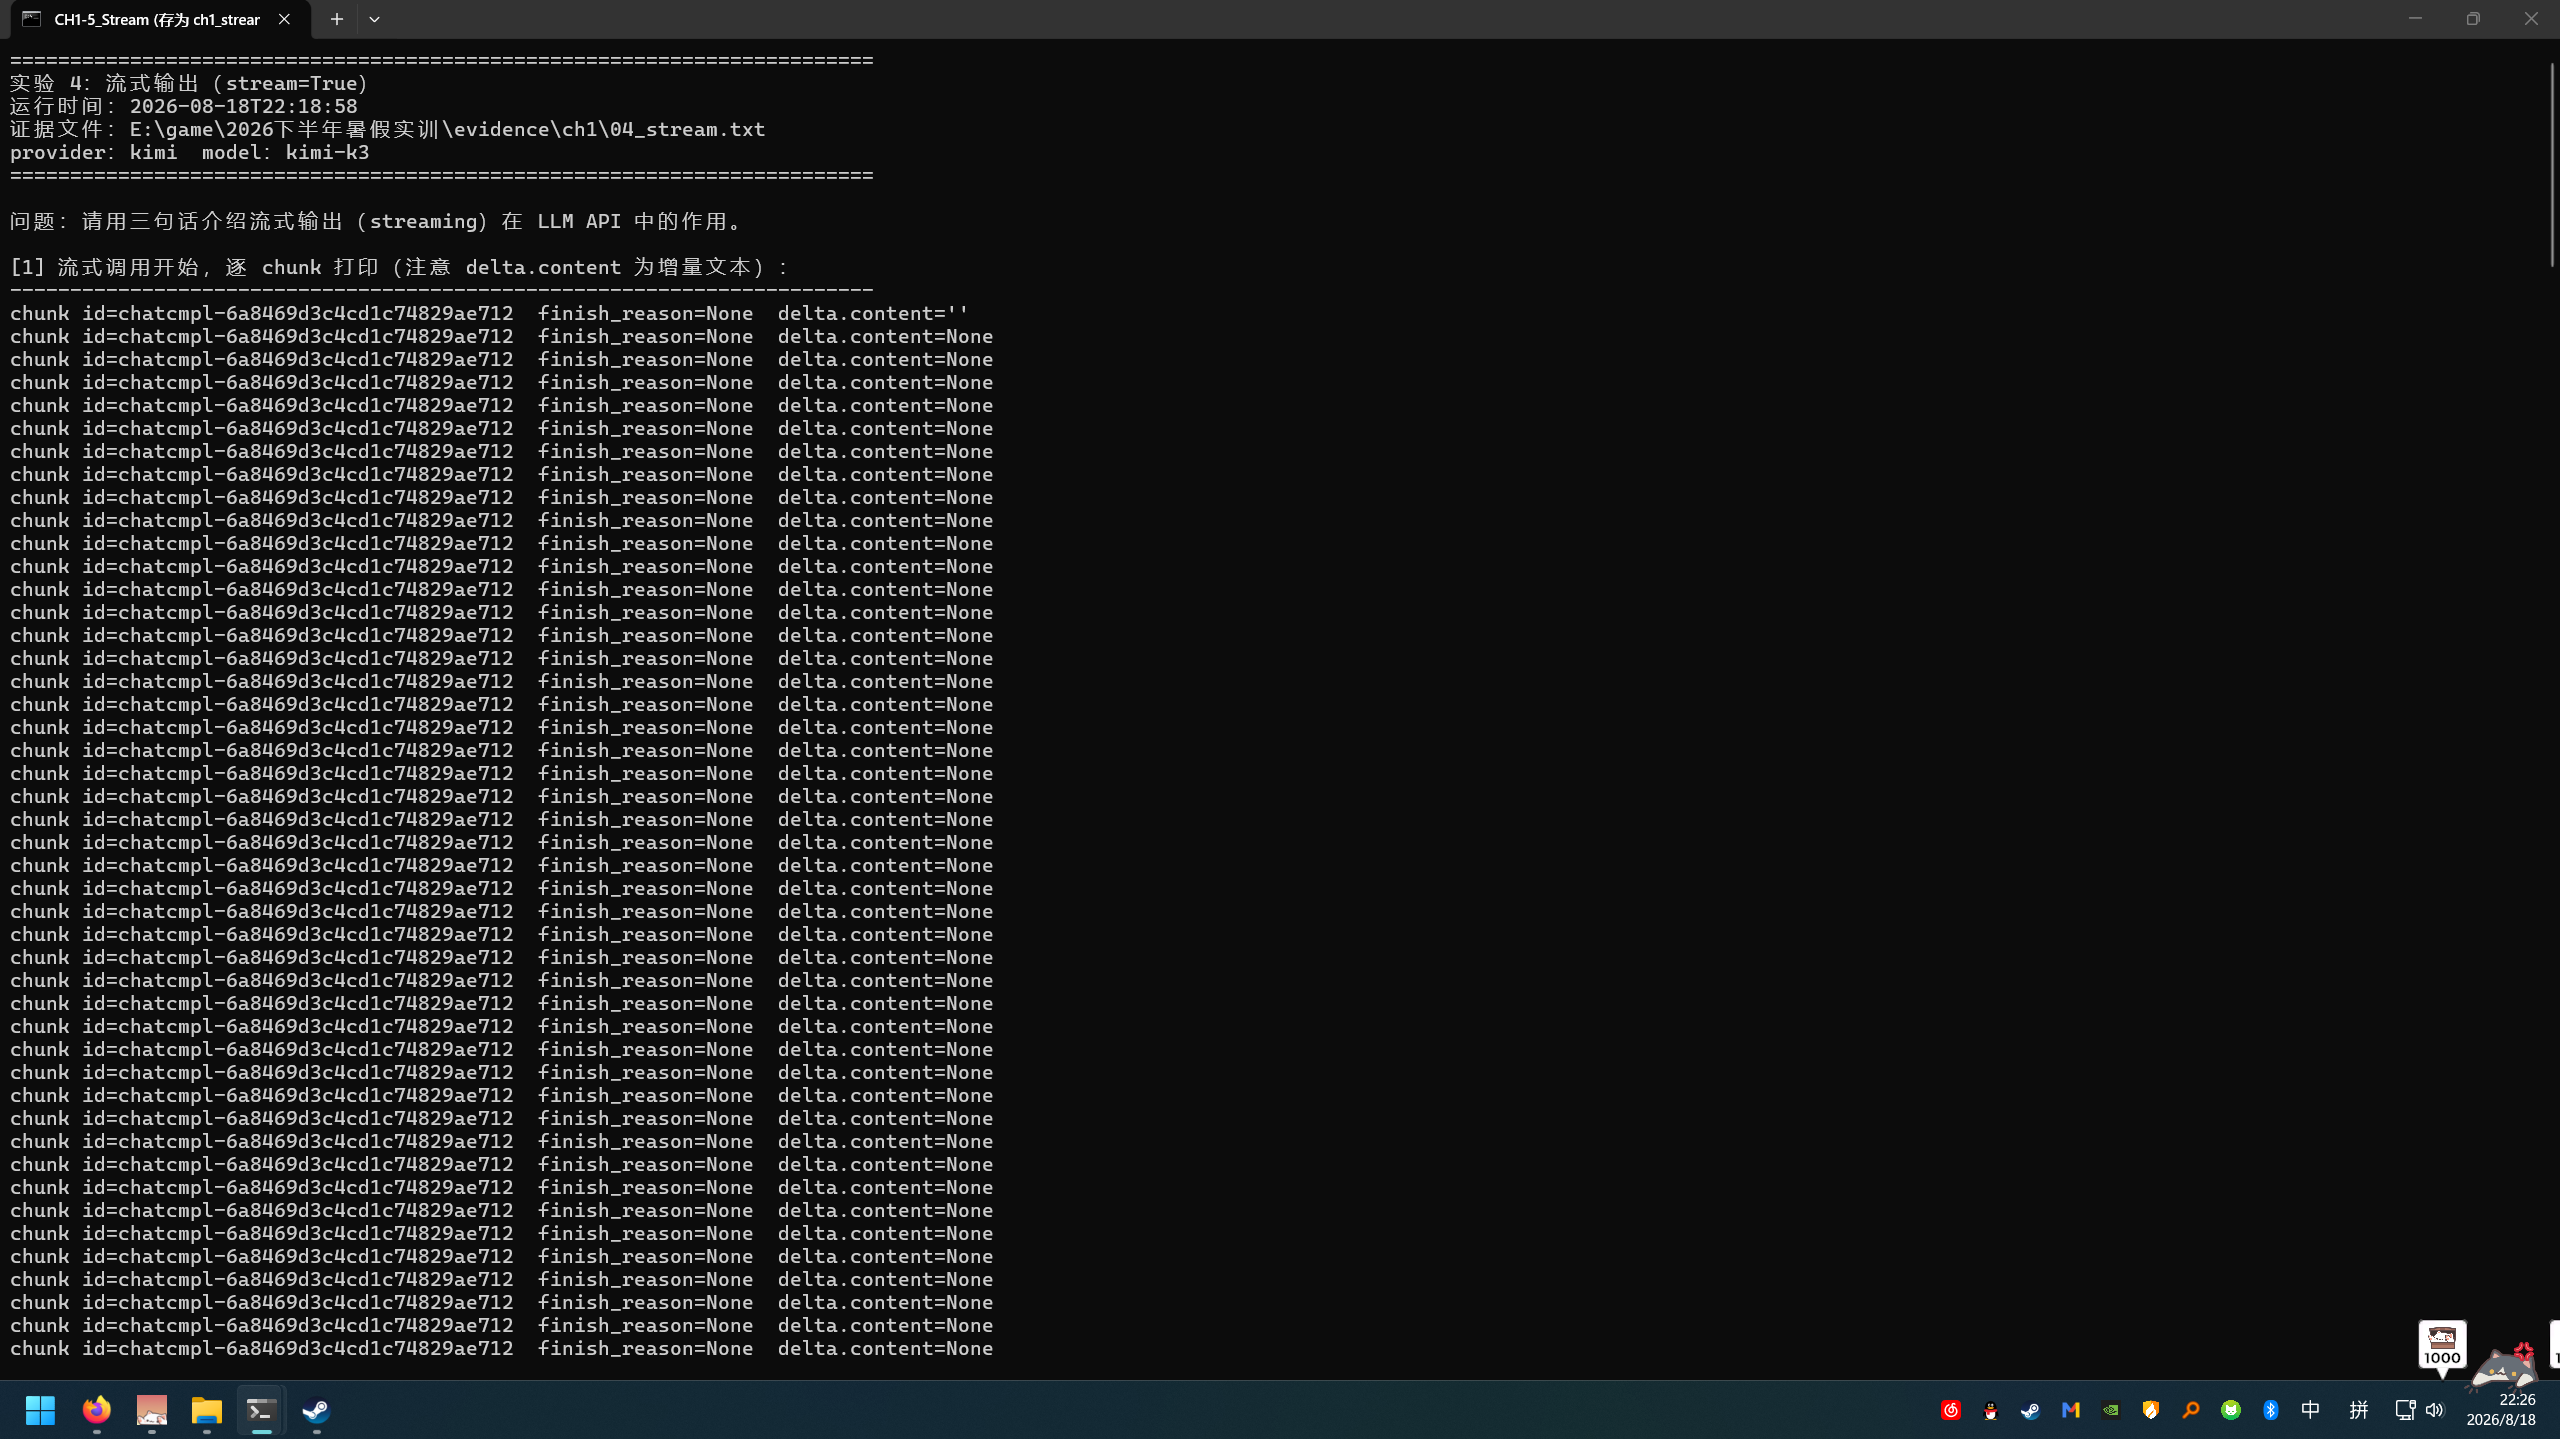
\includegraphics[width=0.92\textwidth]{ch1_stream1.png}
\caption{实验 4：流式输出真实运行窗口——前段为推理阶段 chunk（正文为空），后段为正文逐字 chunk（结构见上文代码块）。}
\label{fig:ch1_stream_chunks}
\end{figure}

\begin{figure}[H]
\centering
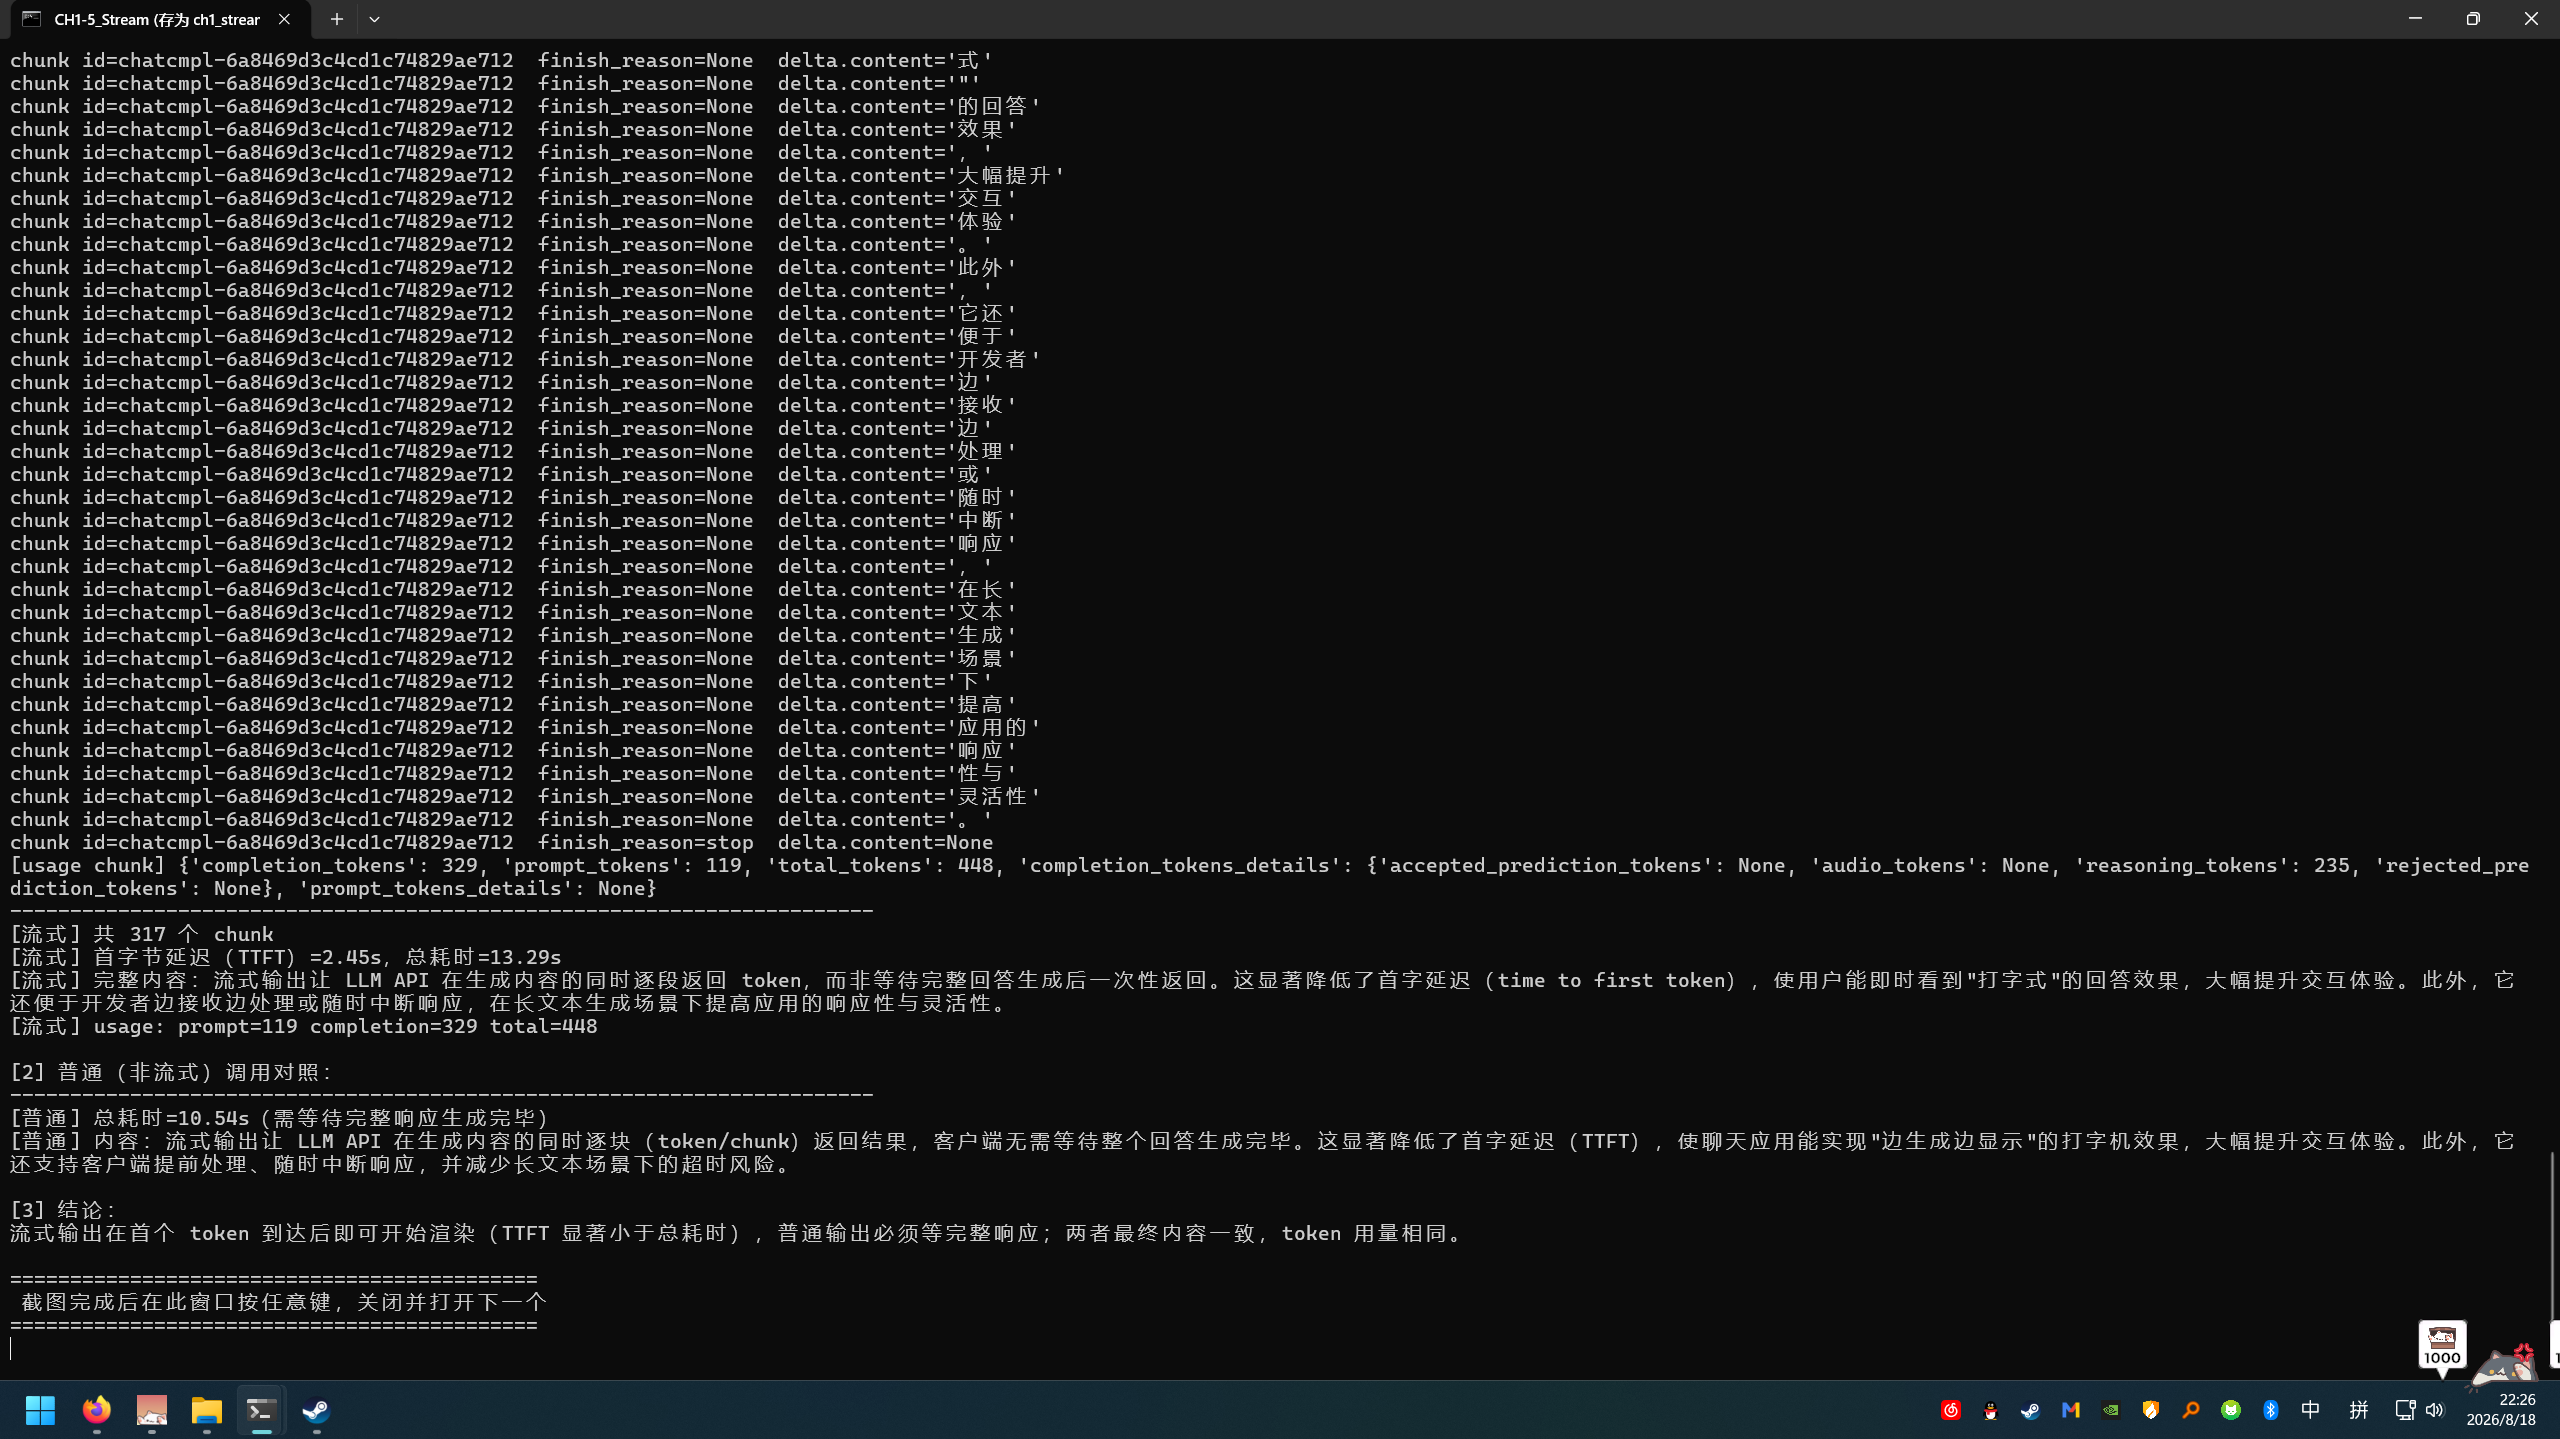
\includegraphics[width=0.92\textwidth]{ch1_stream3.png}
\caption{实验 4：流式汇总（chunk 数、TTFT、usage）与普通调用对照的真实运行窗口。}
\label{fig:ch1_stream_summary}
\end{figure}

\subsubsection{实验 5 结果：JSON 输出与校验}

kimi-k3 在 \texttt{response\_format=\{"type":"json\_object"\}} 下输出合法的
课程计划 JSON，\texttt{json.loads} 解析成功，四个字段（\texttt{title}、
\texttt{tasks}、\texttt{deadline}、\texttt{risks}）全部通过结构校验，且
\texttt{tasks}（5 项）与 \texttt{risks}（4 项）满足数量要求：

\begin{verbatim}
{
  "title": "学生大模型 API 调用实战教程",
  "tasks": [
    "注册大模型平台账号并获取 API Key，完成环境变量配置",
    "使用 Python 编写第一个 API 调用脚本，实现基础文本生成",
    ...],
  "deadline": "2025-06-30",
  "risks": [
    "API 调用超出免费额度产生意外费用",
    "API Key 泄露导致账号被盗用", ...]
}
[json.loads] 解析成功
[结构校验] 通过
\end{verbatim}

真实运行窗口见图~\ref{fig:ch1_json}。补充实验（\nolinkurl{test_mimo_json.py}，证据
\nolinkurl{05b_mimo_json_behavior.txt}）表明：MiMo 在非流式 + json\_object、
非流式 + 纯提示词约束、流式 + json\_object 三种方式下均可输出可解析 JSON，
但在实验 7 的对比调用中偶发输出 \texttt{```json} Markdown 围栏（详见
对比分析）。

\begin{figure}[H]
\centering
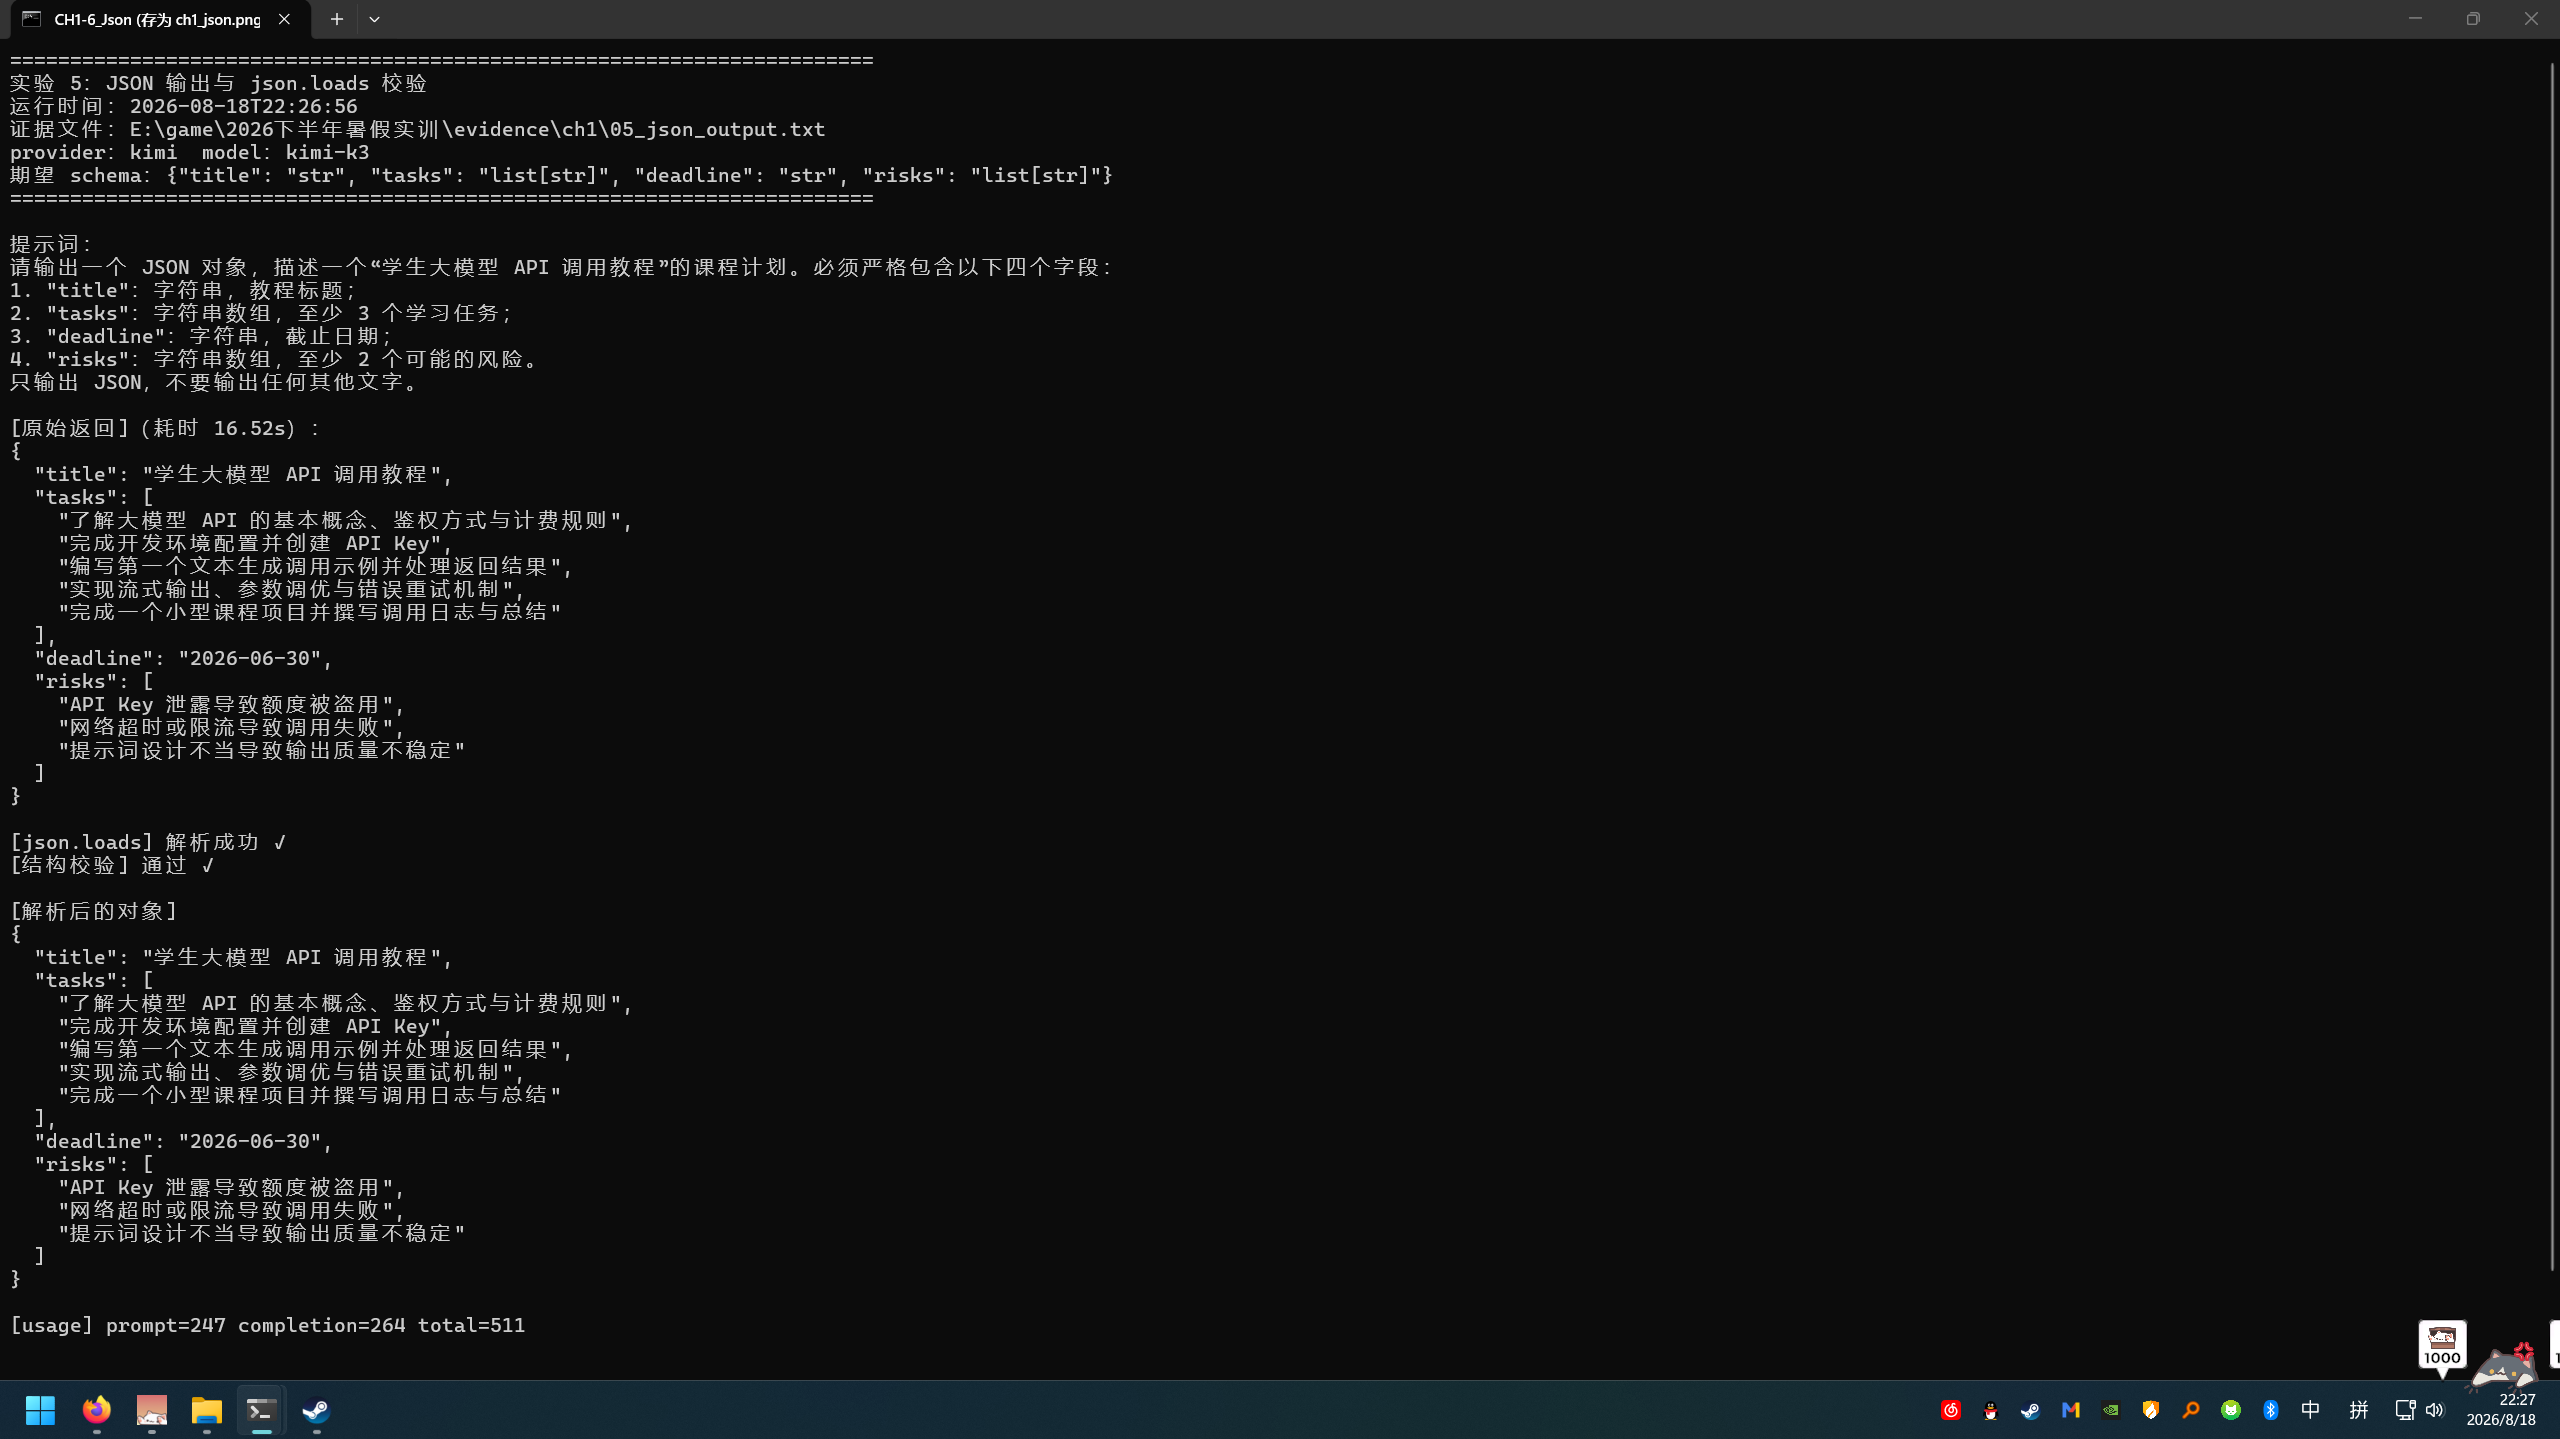
\includegraphics[width=0.92\textwidth]{ch1_json.png}
\caption{实验 5：JSON 输出与 \texttt{json.loads} 校验的真实运行窗口，校验与结构检查均通过。}
\label{fig:ch1_json}
\end{figure}

\subsubsection{实验 6 结果：错误处理}

四类故意触发的错误全部按预期返回，见表~\ref{tab:ch1_errors}。Kimi 的错误
体遵循 OpenAI 风格（\texttt{error.message} 与 \texttt{error.type} 字段），
base\_url 错误时返回的是平台自定义格式（\texttt{code:5}、
\texttt{error:url.not\_found}）。

\begin{table}[H]
\centering
\caption{错误处理实验结果（kimi-k3）}
\label{tab:ch1_errors}
\small
\begin{tabular}{cllp{4.2cm}}
\toprule
\textbf{场景} & \textbf{异常类型} & \textbf{HTTP 状态码} & \textbf{服务端错误信息} \\
\midrule
错误 API key & AuthenticationError & 401 & Invalid Authentication \\
错误模型名 & NotFoundError & 404 & Not found the model ... or Permission denied \\
错误 base\_url & NotFoundError & 404 & code:5, url.not\_found \\
请求体缺 messages & BadRequestError & 400 & Invalid request: messages must not be empty \\
\bottomrule
\end{tabular}
\end{table}

排查要点：401 检查 key 是否有效/权限；400 检查请求体与 model 拼写；
404 检查 base\_url 路径；429（限流）需要退避重试。真实运行窗口见图~\ref{fig:ch1_errors}。

\begin{figure}[H]
\centering
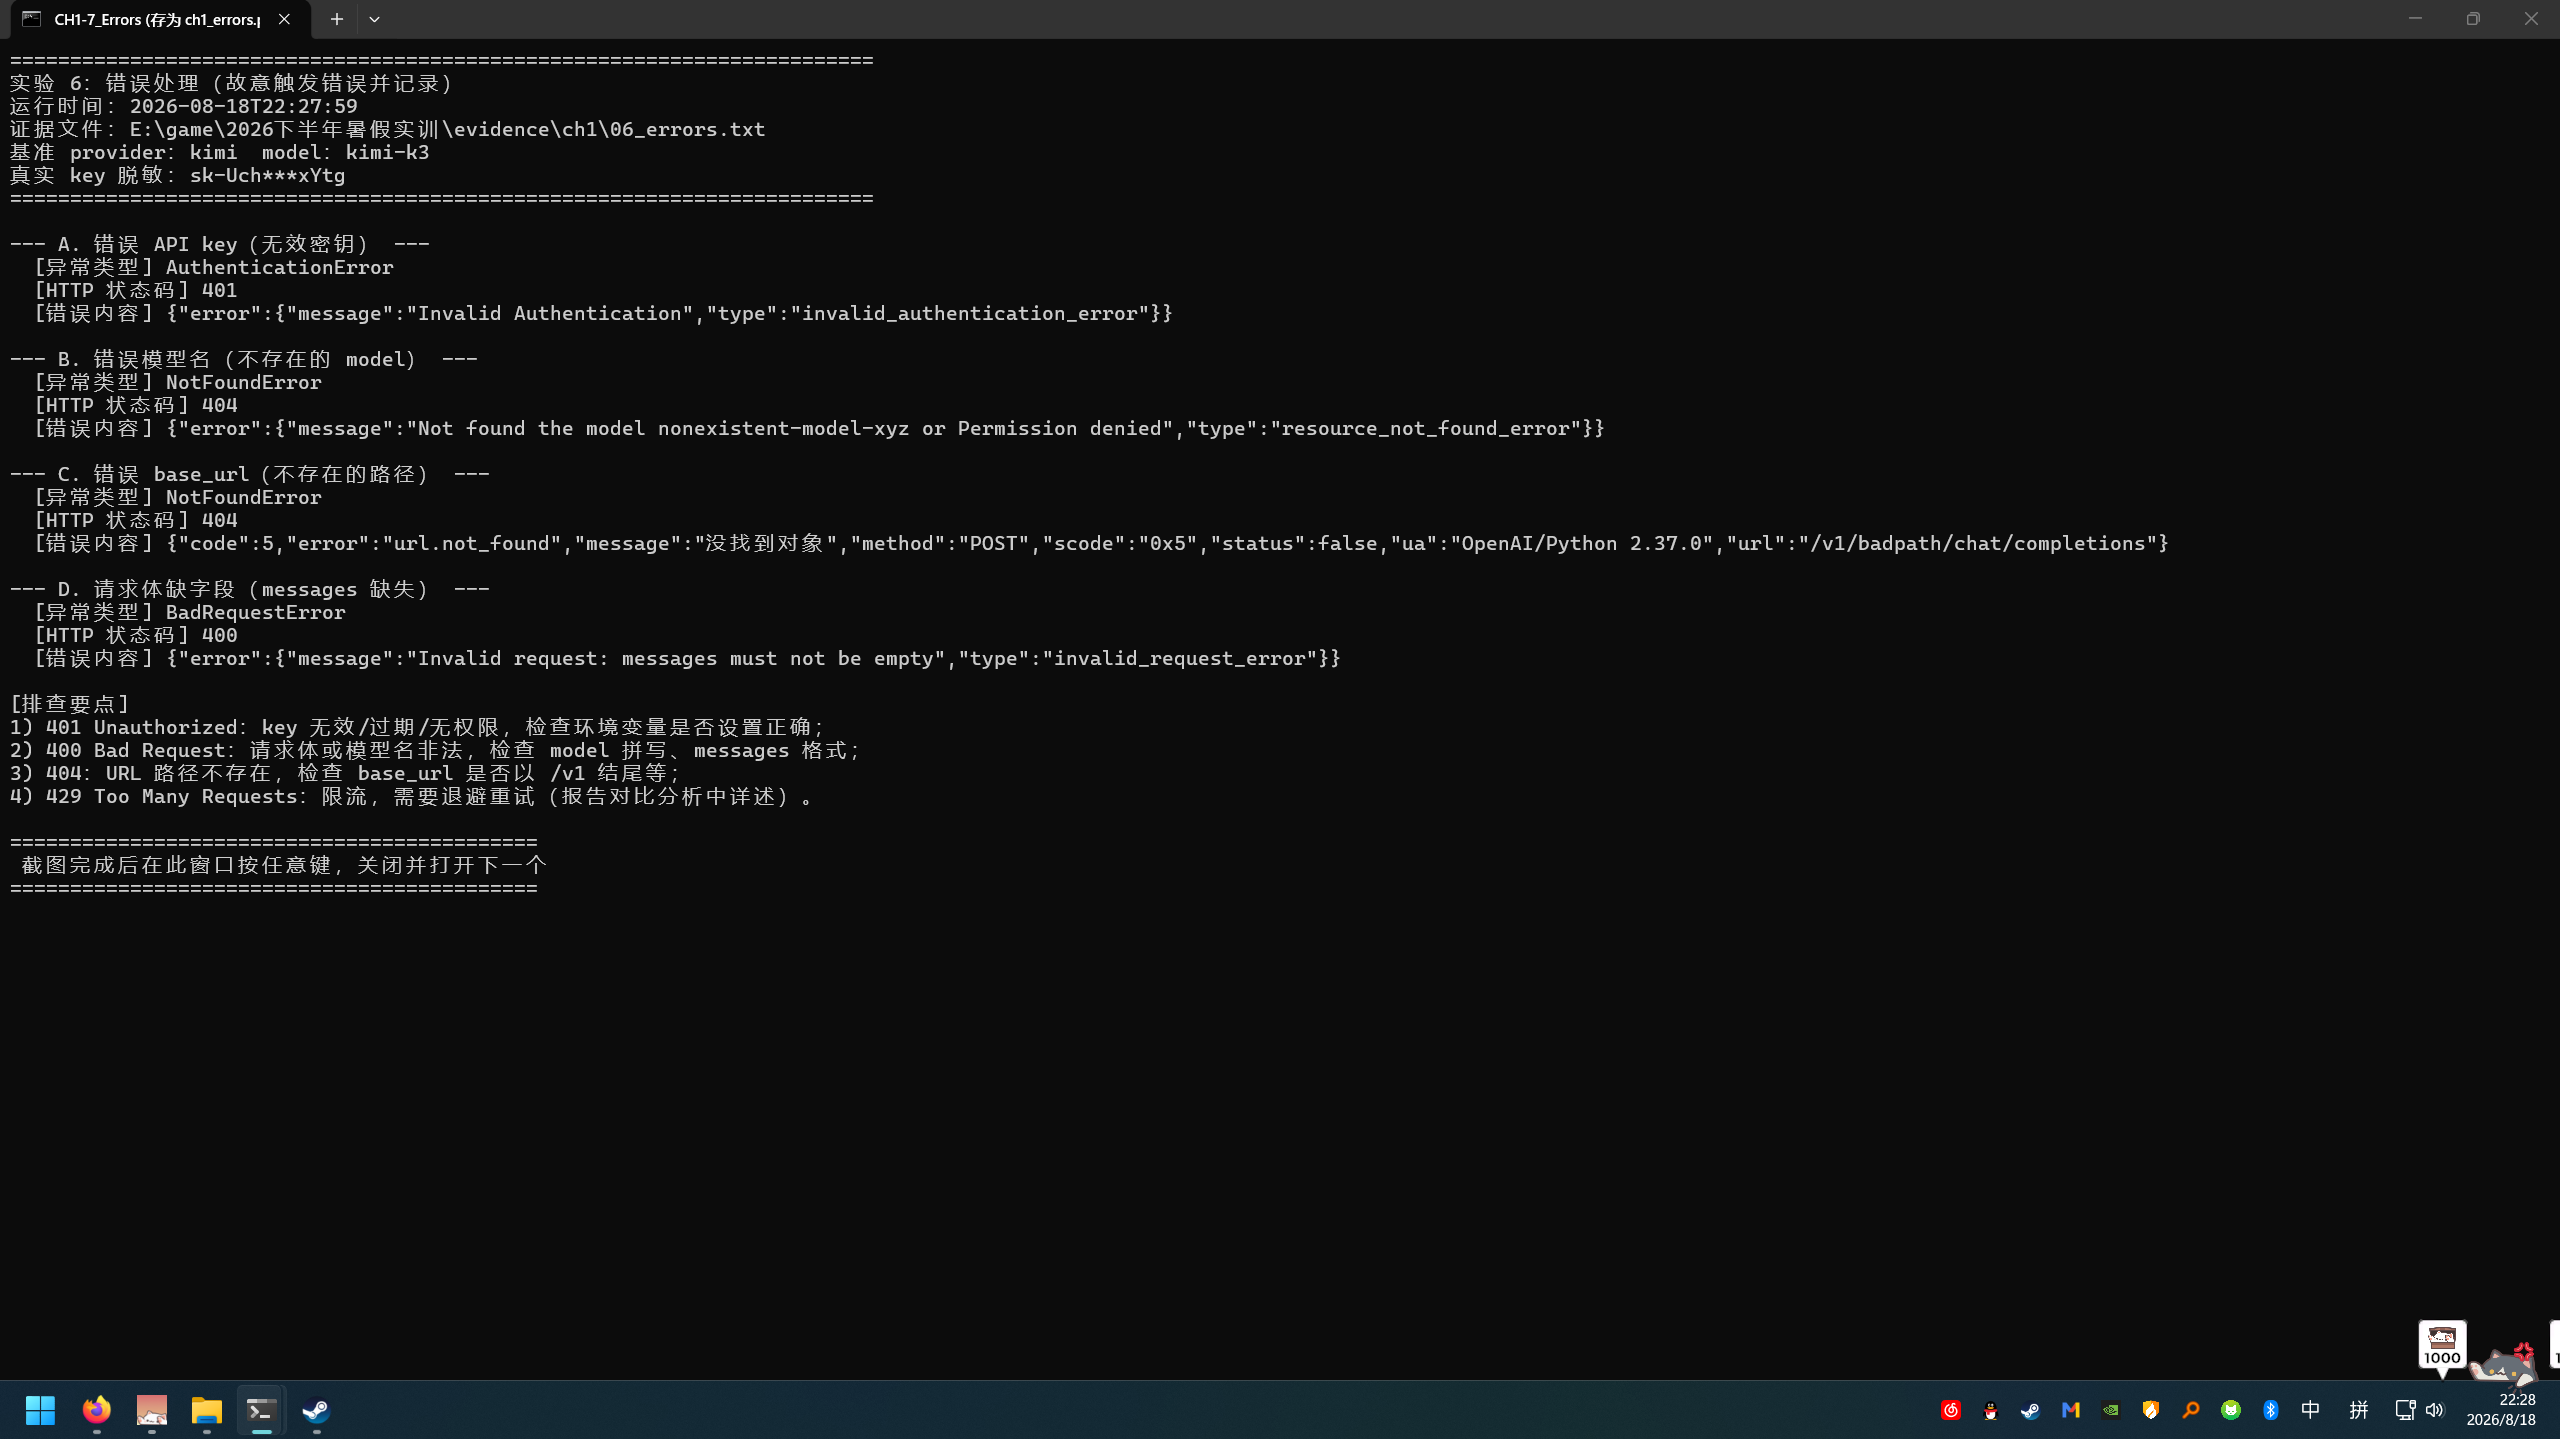
\includegraphics[width=0.92\textwidth]{ch1_errors.png}
\caption{实验 6：四类错误（401/404/404/400）的真实运行窗口，含异常类型与服务端错误信息。}
\label{fig:ch1_errors}
\end{figure}

\subsubsection{实验 7 结果：模型对比}

同一中文任务（JSON 格式学习计划）流式调用两个模型，结果见表~\ref{tab:ch1_compare}
与图~\ref{fig:ch1_compare}（延迟柱状图）、图~\ref{fig:ch1_compare_terminal}
（运行窗口对比摘要）。MiMo 的 TTFT 更短（0.90 s），但本次调用总耗时
更长且 JSON 输出带 Markdown 围栏导致直接解析失败；Kimi 输出稳定。

\begin{table}[H]
\centering
\caption{模型对比结果（同一中文任务，流式）}
\label{tab:ch1_compare}
\small
\begin{tabular}{lcc}
\toprule
\textbf{指标} & \textbf{kimi-k3} & \textbf{mimo-v2.5-pro} \\
\midrule
TTFT (s) & 2.57 & 0.90 \\
总耗时 (s) & 12.82 & 15.80 \\
响应字数 & 362 & 405 \\
JSON 直接可解析 & 是 & 否（输出 \texttt{```json} 围栏） \\
上下文窗口 & 1,048,576（1M） & 1,048,576（1M，最大输出 128K） \\
输出单价（每 1M tokens） & ¥100.00 & ¥6.00 \\
\bottomrule
\end{tabular}
\end{table}

\begin{figure}[H]
\centering
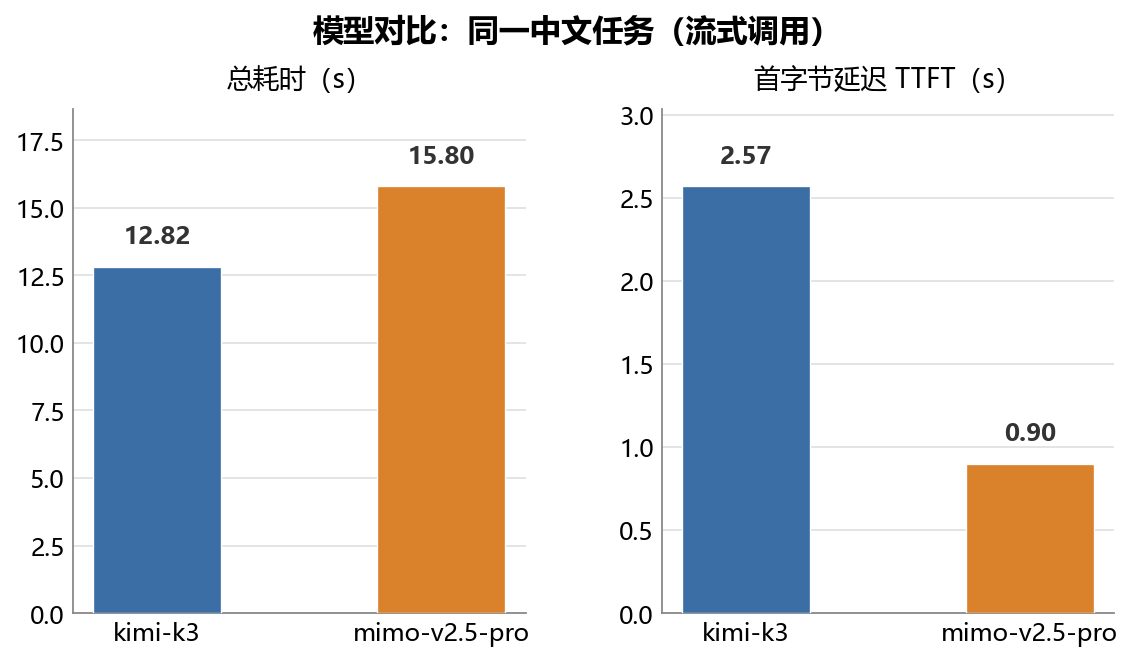
\includegraphics[width=0.92\textwidth]{ch1_model_compare.png}
\caption{模型对比：同一中文任务（流式调用）的总耗时与首字节延迟。}
\label{fig:ch1_compare}
\end{figure}

\begin{figure}[H]
\centering
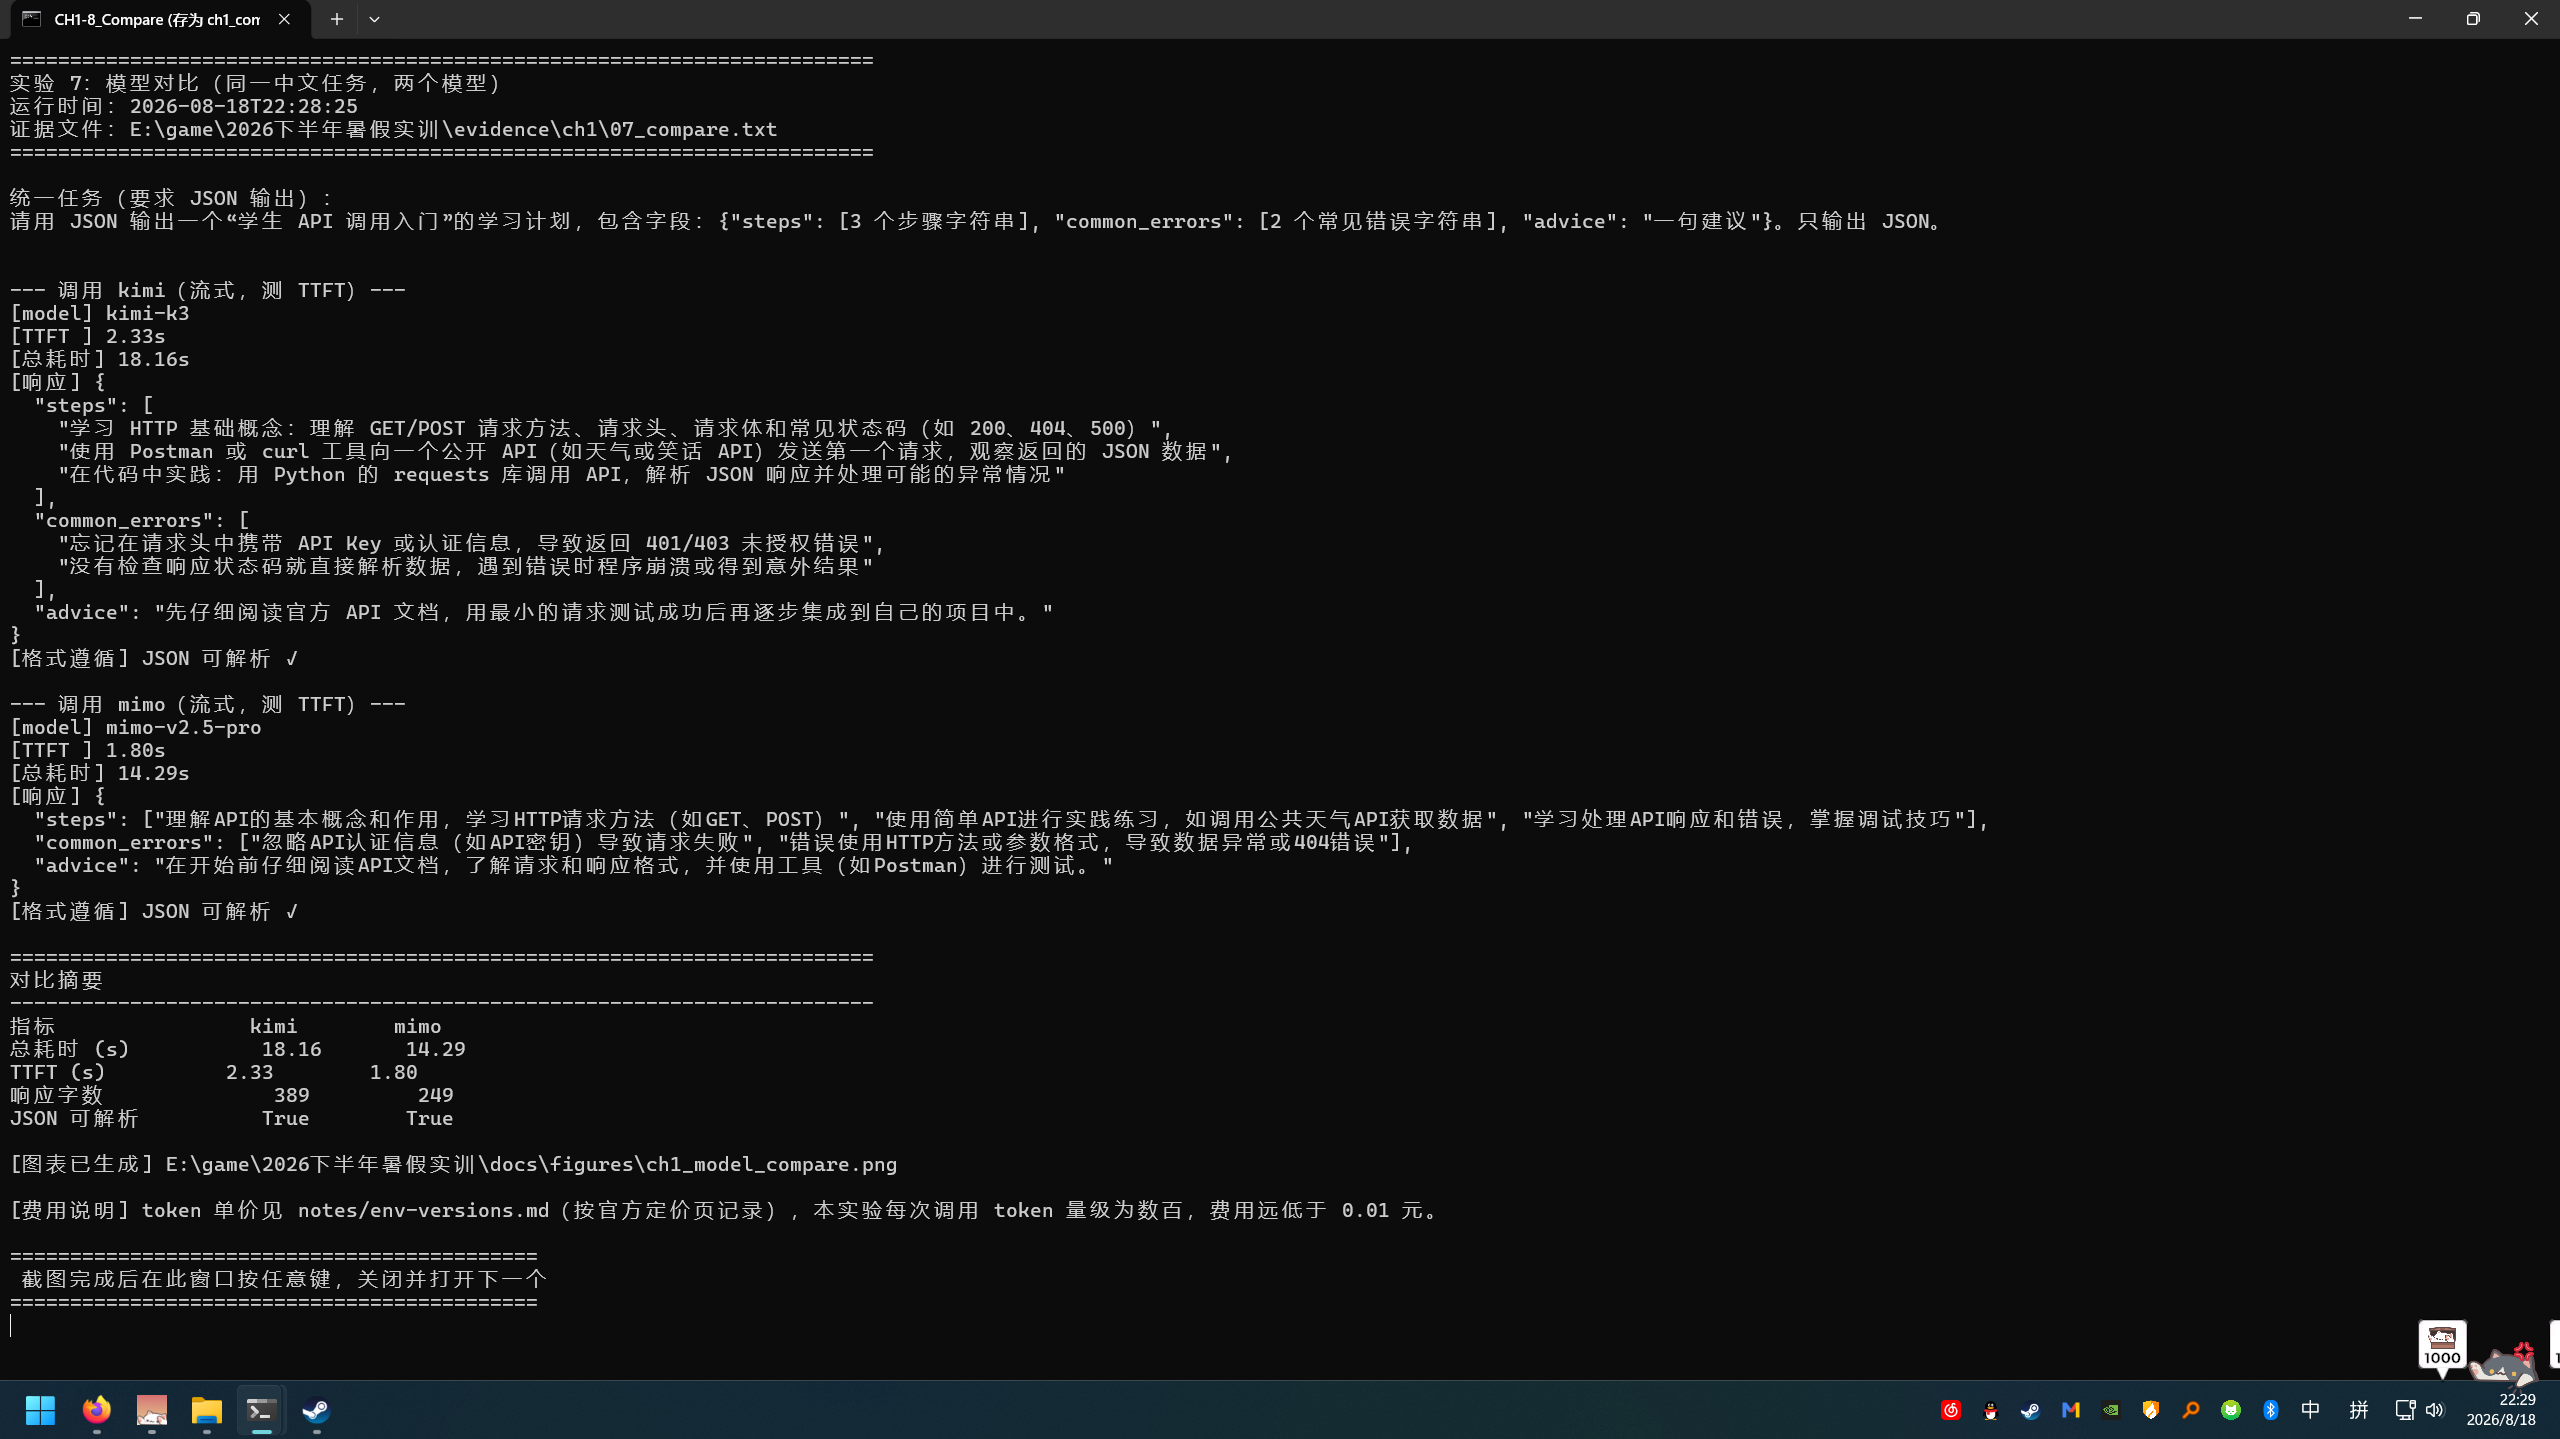
\includegraphics[width=0.92\textwidth]{ch1_compare.png}
\caption{实验 7：模型对比的真实运行窗口（对比摘要：总耗时、TTFT、响应字数、JSON 可解析）。}
\label{fig:ch1_compare_terminal}
\end{figure}

\subsection{对比分析}

\begin{enumerate}[leftmargin=4em,itemsep=0pt,topsep=2pt]
    \item \textbf{响应质量}：两个模型均能准确回答中文技术问题。Kimi 回答更
          详尽（会主动补充 \texttt{Content-Type} 等技术细节），MiMo 更简洁。
          在 JSON 学习计划任务中两者输出内容质量相当（均覆盖步骤、常见错误
          与建议三个要素）。
    \item \textbf{格式遵循}：Kimi 在 json\_object 模式下输出稳定、无多余内容；
          MiMo 偶发在 JSON 外加 \texttt{```json} Markdown 围栏（补充实验中
          三种方式均可解析，说明是采样不稳定而非能力缺失）。工程建议：
          解析前先剥离代码块围栏，或解析失败时重试一次。
    \item \textbf{速度}：实验 3 中 MiMo 总耗时（4.78 s）明显快于 Kimi
          （11.91 s）；实验 7 中两者总耗时接近（12.8 s vs 15.8 s），但 MiMo
          TTFT（0.90 s）快于 Kimi（2.57 s）。推理模型的延迟受推理长度影响，
          波动较大，单次测量只能作为量级参考。两个模型均为推理模型，
          completion\_tokens 中推理 token 占比高（Kimi 可达 70\%+），调用
          推理模型时 \texttt{max\_tokens} 必须预留推理空间。
    \item \textbf{费用}：按官方定价（Kimi K3：输入 ¥20/M、缓存命中 ¥2/M、
          输出 ¥100/M；MiMo v2.5-pro：输入 ¥3/M、缓存命中 ¥0.025/M、输出
          ¥6/M，均以每 1M tokens 计），用各实验日志中的真实 usage 计算
          （公式：费用 = prompt×输入单价/1e6 + completion×输出单价/1e6，
          缓存未命中保守口径），汇总见表~\ref{tab:ch1_cost}。第 1 章全部
          API 调用总费用约 ¥0.169 元（kimi ≈ ¥0.165、mimo ≈ ¥0.004），
          远低于 0.5 元。需要指出的是：推理模型的推理 token 计入
          completion\_tokens 一并计费（Kimi 的 reasoning 占比高，是费用
          较高的主因）；MiMo 的提示词缓存（cached\_tokens）可进一步降低
          重复调用成本。单价与 usage 明细见 \nolinkurl{evidence/ch1/08_cost_summary.txt}。

\begin{table}[H]
\centering
\caption{第 1 章 API 调用费用汇总（官方单价 × 真实 usage，2026-08-18）}
\label{tab:ch1_cost}
\small
\setlength{\tabcolsep}{4pt}
\begin{tabular}{lrrr}
\toprule
\textbf{实验/调用} & \textbf{prompt} & \textbf{completion} & \textbf{费用（元）} \\
\midrule
实验 2 curl Kimi（完整） & 100 & 393 & 0.0413 \\
实验 2 curl Kimi（截断） & 100 & 150 & 0.0170 \\
实验 2 curl MiMo（完整） & 264 & 84 & 0.0013 \\
实验 2 curl MiMo（截断） & 264 & 150 & 0.0017 \\
实验 3 统一调用 kimi & 122 & 380 & 0.0404 \\
实验 3 统一调用 mimo & 37 & 99 & 0.0007 \\
实验 4 流式（kimi） & 119 & 329 & 0.0353 \\
实验 5 JSON（kimi） & 247 & 264 & 0.0313 \\
\midrule
kimi-k3 合计 & & & ≈ 0.1654 \\
mimo-v2.5-pro 合计 & & & ≈ 0.0037 \\
\textbf{总计} & & & \textbf{≈ 0.1691} \\
\bottomrule
\end{tabular}

\par\vspace{3pt}
\begin{center}
{\footnotesize 注：费用按缓存未命中保守口径估算（公式见对比分析第 4 条）。
其中 3 次调用在日志中检出上下文缓存命中（curl Kimi 完整 cached\_tokens=100、
curl MiMo 完整 256、curl MiMo 截断 192），若这三行改按缓存单价核算，
全章总费用约 ¥0.166（比保守口径低约 ¥0.003）。明细见
\nolinkurl{evidence/ch1/08_cost_summary.txt}。}
\end{center}
\end{table}

    \item \textbf{上下文长度}：两模型上下文窗口均为 1M
          （1,048,576 tokens；MiMo 最大输出 131,072），长文本/整库检索场景
          均无需分块。差异在于：Kimi 始终推理且输出单价高，长上下文大输出
          场景成本显著高于 MiMo；MiMo 输出上限（128K）低于 Kimi 的完整
          1M 输出空间（Kimi 输出上限以官方文档为准），超长生成任务需注意。
    \item \textbf{限流与错误恢复}：Kimi 的错误体为标准 OpenAI 格式，易于
          程序化解析；MiMo 未实测 429（本章未触发限流）。两个平台均返回
          HTTP 状态码，配合 OpenAI SDK 的异常类型（AuthenticationError /
          NotFoundError / BadRequestError）可直接定位问题。
    \item \textbf{文档易用性}：Kimi（platform.moonshot.cn）与小米 MiMo
          （mimo.mi.com）均提供 OpenAI-compatible 快速开始文档；MiMo 文档
          明确标注思考模式下 temperature/top\_p 无效，Kimi 需要从文档中
          确认 kimi-k3 的推理特性。整体上两者的接入成本相近，均只需
          base\_url + key + model 三项配置。
\end{enumerate}

\subsection{可复现教程}

本章实验的全部脚本位于 \texttt{code/ch1-api/}，复现步骤为：

\begin{enumerate}[leftmargin=4em,itemsep=0pt,topsep=2pt]
    \item 复制 \texttt{.env.example} 为 \texttt{.env}，填入至少两个平台的 API key；
    \item 使用 Miniconda ML-base 环境（Python 3.11.15），按
          \texttt{requirements.txt} 安装依赖（\texttt{pip install -r}
          \texttt{ requirements.txt}）；
    \item 依次运行：\texttt{unified\_call.py kimi mimo}、
          \texttt{stream\_call.py kimi}、\texttt{json\_output.py kimi}、
          \texttt{error\_cases.py kimi}、\texttt{compare\_models.py kimi mimo}；
    \item 每个脚本自动把真实输出写入 \texttt{evidence/ch1/}（UTF-8 日志）。
\end{enumerate}

\begin{thebibliography}{9}

\bibitem{kimi-doc}
Moonshot AI. Kimi API 快速开始[EB/OL].
\url{https://platform.moonshot.cn/docs/guide/start-using-kimi-api}，
访问日期 2026-08-17.

\bibitem{qwen-doc}
阿里云. 阿里云百炼首次调用千问 API[EB/OL].
\url{https://help.aliyun.com/zh/model-studio/getting-started/first-api-call-to-qwen}，
访问日期 2026-08-17.

\bibitem{ark-doc}
火山引擎. 火山方舟快速入门[EB/OL].
\url{https://www.volcengine.com/docs/82379/1298454}，
访问日期 2026-08-17.

\bibitem{mimo-doc}
小米. Xiaomi MiMo API 开放平台——首次调用[EB/OL].
\url{https://mimo.mi.com/docs/zh-CN/quick-start/summary/first-api-call}，
访问日期 2026-08-18.

\bibitem{mdn-http}
MDN. Overview of HTTP[EB/OL].
\url{https://developer.mozilla.org/en-US/docs/Web/HTTP/Overview}，
访问日期 2026-08-17.

\bibitem{rfc8259}
Bray T. The JavaScript Object Notation (JSON) Data Interchange Format:
RFC 8259[S]. IETF, 2017.
\url{https://datatracker.ietf.org/doc/html/rfc8259}，
访问日期 2026-08-17.

\bibitem{curl-doc}
curl. curl official site[EB/OL].
\url{https://curl.se/}，访问日期 2026-08-17.

\bibitem{openai-sdk}
OpenAI. OpenAI Python API library[EB/OL].
\url{https://github.com/openai/openai-python}，访问日期 2026-08-17.

\end{thebibliography}

% ============================================================
%  第二章：提示词到智能体的演化
% ============================================================
\clearpage
\section{第二章：提示词到智能体的演化}

\subsection{背景}

prompt engineering 解决的是``如何问''的问题，适合单次任务和短链路任务。
随着任务变长，模型需要看到项目文件、约束、历史、工具说明、测试结果和外部
数据，于是问题变成``模型应该看到什么''，这就是 context engineering。再往后，
模型不仅要看，还要行动：读文件、写文件、跑命令、搜索、调用 API、开子任务，
这需要 harness engineering。最后，多步任务必须不断观察结果、修正计划、判断
是否结束，这才进入 loop agent。

演化的内在逻辑：任务复杂度越高、时间跨度越长、外部环境越真实、错误代价
越大，工程重心就越从``写好一句 prompt''转向``管理上下文、约束工具、记录
状态、验证结果和设计循环''。本章用一个真实任务（写一份``学生 API 调用
入门教程''）做四层递进实验，量化每一层带来的变化。

\subsection{概念背景：四层各控制什么}

\begin{table}[H]
\centering
\caption{四个 engineering 层级：工程对象与解决的问题}
\label{tab:ch2_levels}
\small
\setlength{\tabcolsep}{4pt}
\begin{tabular}{p{2.5cm}p{4.2cm}p{4.2cm}p{3.2cm}}
\toprule
\textbf{层级} & \textbf{工程对象} & \textbf{主要解决问题} & \textbf{控制面} \\
\midrule
Prompt & 一条/一组指令、示例、输出格式约束 & 让单次模型调用更稳定、更符合格式 & 怎么问 \\
Context & 模型本次采样能看到的全部 token & 在有限上下文内放入``刚好需要''的信息 & 看什么 \\
Harness & 模型外部的运行时：工具、权限、沙箱、日志、检查器 & 让模型能安全感知环境、行动、被约束、被验证 & 能做什么 \\
Loop agent & ``观察 - 思考 - 调工具 - 观察 - 判断是否继续'' 的控制循环 & 处理多步、长时、不确定、需反馈修正的任务 & 何时停 \\
\bottomrule
\end{tabular}
\end{table}

四个层级不是替代关系，而是外层包住内层（图~\ref{fig:ch2_evolution}）：
loop 的每一轮都需要 harness 提供工具与约束，harness 的每一次模型请求都
需要 context 提供材料，context 的组织方式又由 prompt 的结构决定。

\subsubsection{为什么 context 不是把资料全部塞进 prompt}

上下文包不采用``全量投射''而是``精选摘要 + 引用''，原因有四：
\begin{enumerate}[leftmargin=4em,itemsep=0pt,topsep=2pt]
    \item \textbf{有限上下文窗口}：token 预算有限，全量放入必然挤压
          任务相关信息的空间；
    \item \textbf{信息污染}：无关材料会让模型跑偏（工程语境称 context rot，
          上下文腐化），文档里与任务无关的章节、广告话术都是噪音；
    \item \textbf{成本与延迟}：token 越多费用与耗时越高（第 1 章费用
          记录：费用 = token $\times$ 单价，上下文占用量直接计价）；
    \item \textbf{可维护性}：资料有版本与来源，全量塞入无法逐项标注
          更新策略；正确做法是把``刚好需要''的信息按来源摘要进上下文，
          完整文档放在文件系统/检索里按需取用——这正是本章上下文包的
          设计（官方文档摘要 + 学生画像 + 模板要求，每项标注来源）。
\end{enumerate}

\subsubsection{为什么工具说明也是 prompt/context 的一部分}

模型只有``看到''工具说明（名字、参数、用途、输出约定与使用时机），
才能决定是否调用、如何填参数。工具说明随注册进入系统提示词组装
（第 4 章验证：注册工具 schema 自动流入系统提示词——``schemas flow
into the system-prompt assembly automatically''），因此工具说明本质上
是 context engineering 的对象：参数描述清晰、用途边界明确的说明，
模型才用得对；工具说明含糊（参数含义不明、无输出约定）会导致模型
反复试错、填错参数甚至干脆不用工具。

\begin{figure}[H]
\centering
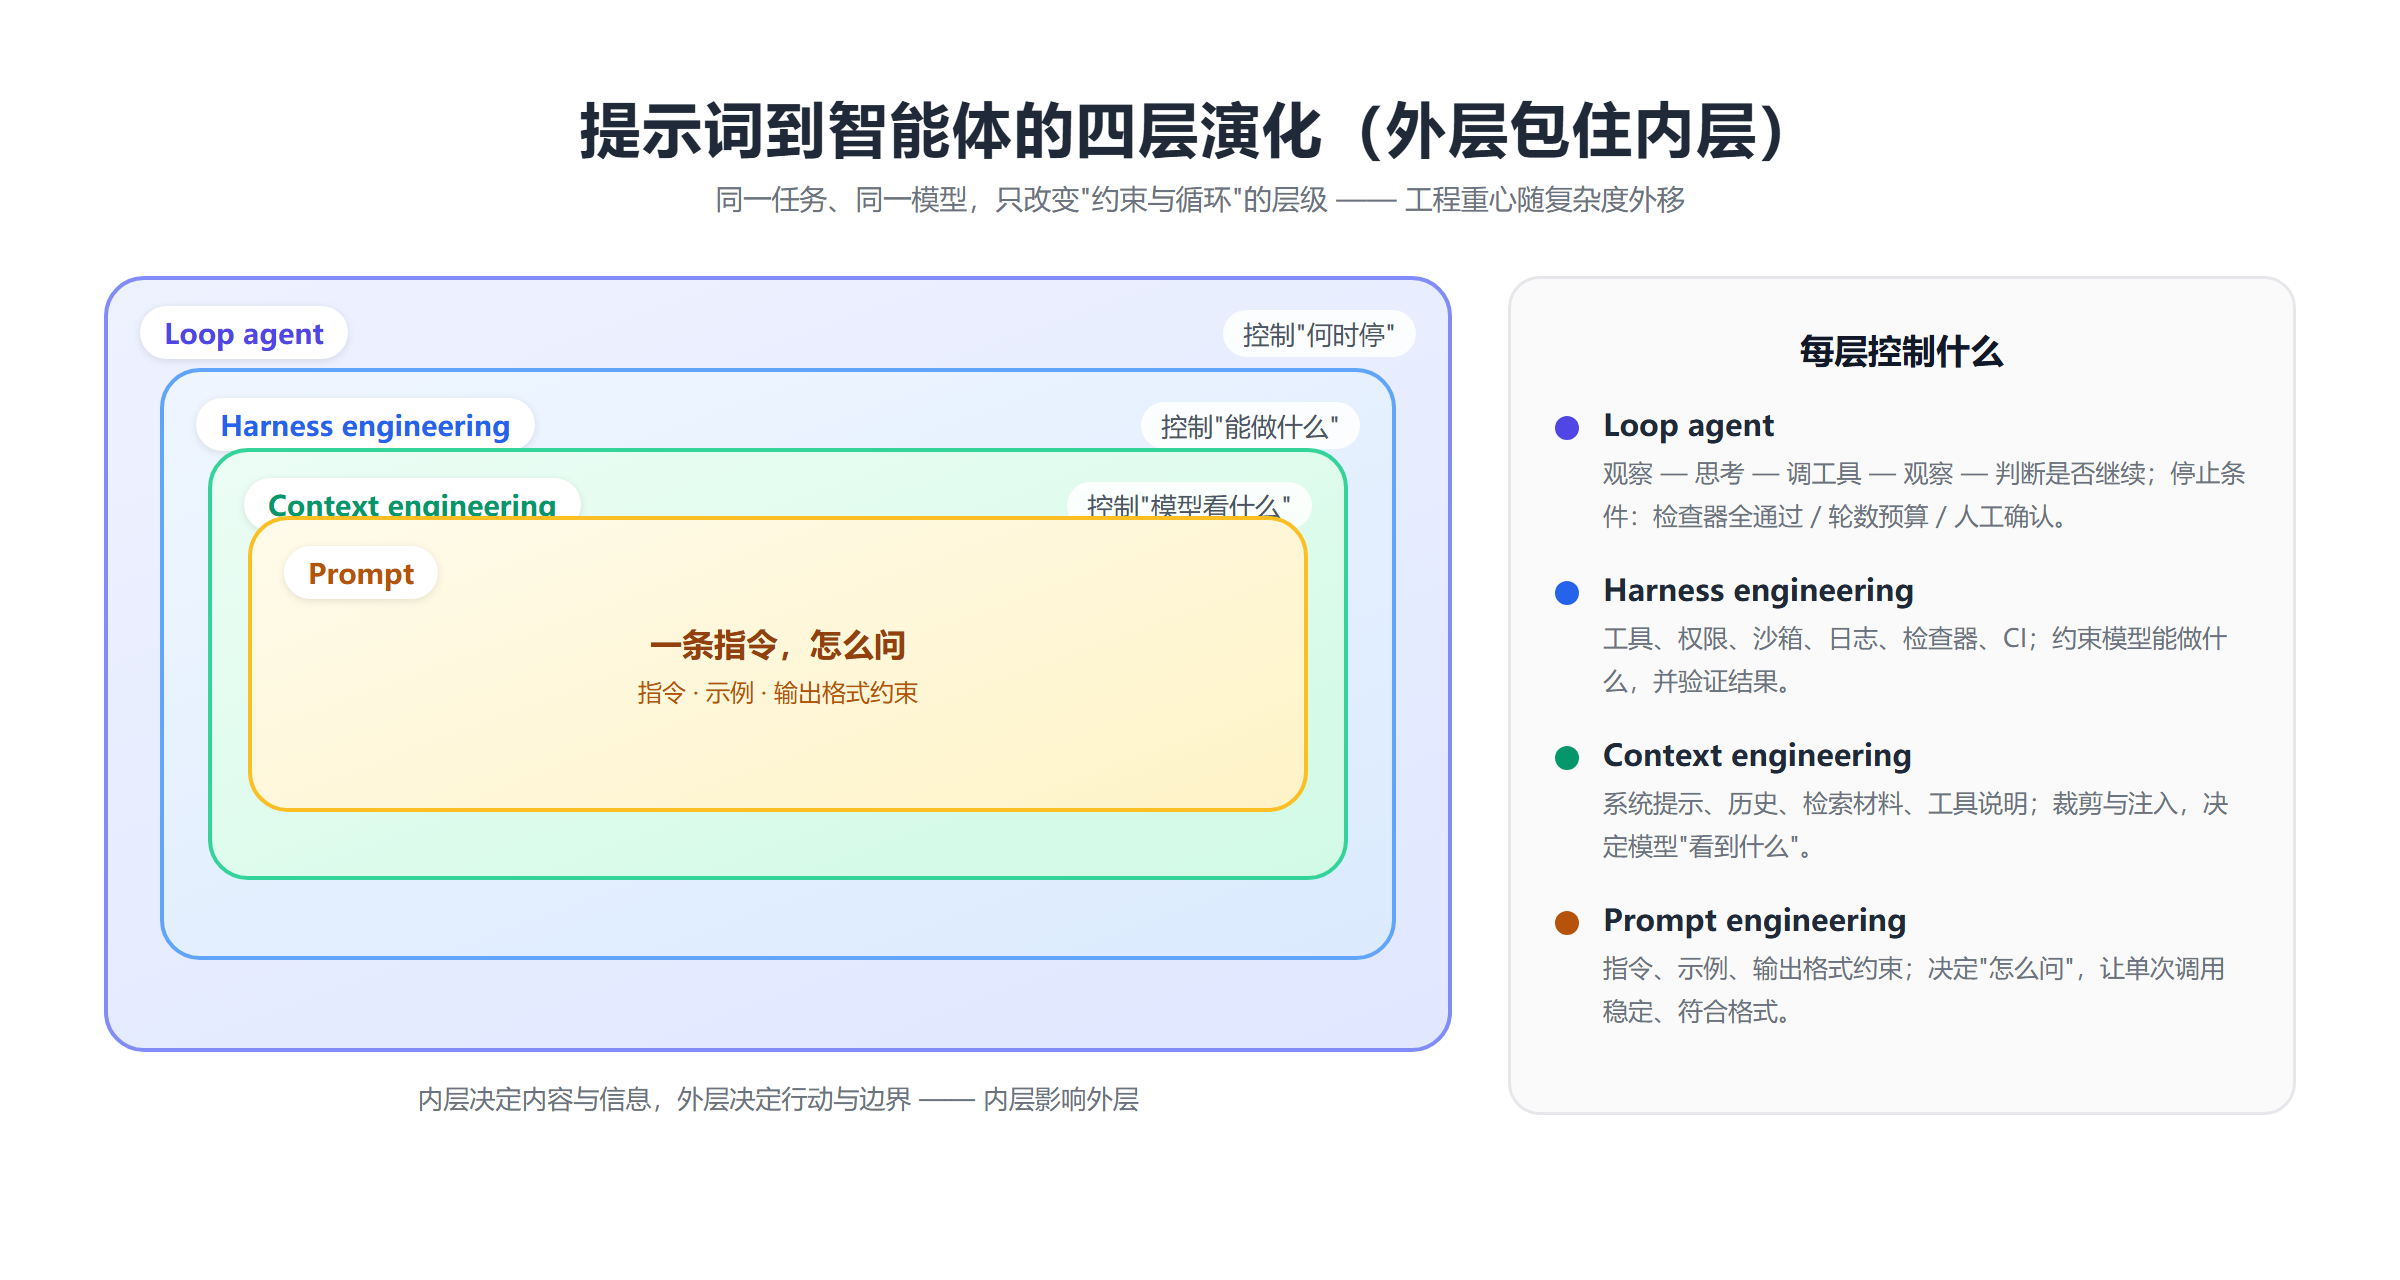
\includegraphics[width=0.85\textwidth]{ch2_evolution.png}
\caption{prompt → context → harness → loop agent 四层嵌套演化示意。}
\label{fig:ch2_evolution}
\end{figure}

\subsubsection{harness 与 framework、IDE、MCP、plugin、sandbox、CI 的关系}

harness 不是某一个具体技术，而是``模型外部的运行时''这一角色的总称，它与
常见概念的关系是：
\begin{itemize}[leftmargin=4em,itemsep=0pt,topsep=2pt]
    \item \textbf{framework（框架）}：harness 可以用框架实现（如 LangChain/
          Pi/DSH 各自的内核），但框架是软件形态，harness 是职责——同一个
          harness 职责可以由不同框架承载；
    \item \textbf{IDE（Agent IDE / 编辑器）}：IDE 是 harness 能力的交互
          载体——DSH Web UI、CodeBuddy 等把 harness 的工具、会话、审计与
          权限包装成聊天/编辑器界面；IDE 与 harness 是``界面 vs 运行时''
          的关系，同一天 harness 可以驱动不同前端；
    \item \textbf{MCP}：MCP 是工具接入的开放协议（模型-工具之间的标准化
          传输层），harness 是执行环境——harness 通过 MCP 客户端接入外部
          MCP server 的工具，MCP 解决``工具怎么连''，harness 解决``工具
          怎么被安全地调度与验证''；
    \item \textbf{plugin}：插件是 harness 的组合单元——DSH 的
          ``Everything is a plugin'' 表明模型、工具、沙箱、UI 都可作为插件
          挂载进 harness 运行时；
    \item \textbf{sandbox}：沙箱是 harness 的权限边界之一——工具执行的隔离
          环境（文件系统/网络/进程限制），属于 harness engineering 的安全
          约束面；
    \item \textbf{CI}：CI 是 harness 质量保障的延伸——把检查器、回归测试、
          评审流程接入 agent 循环（如第 2 章 loop 层的 rubric 检查器，放大
          到仓库级就是 CI 化的 agent 流水线）。
\end{itemize}

\subsection{实验设计：同一任务四层递进}

\begin{enumerate}[leftmargin=4em,itemsep=0pt,topsep=2pt]
    \item \textbf{Prompt 层}：只给模型一句任务：``写一个面向零基础学生的
          大模型 API 调用入门教程''，无任何额外信息；
    \item \textbf{Context 层}：在系统提示中加入上下文包：Kimi 官方文档摘要
          （申请/调用/计费要点）、OpenAI-compatible 迁移说明、目标学生基础、
          报告模板要求；
    \item \textbf{Harness 层}：保留上下文包，并给模型一套\textbf{真实工具集
          }：\texttt{write\_file}（写入沙箱文件）、\texttt{run\_tests}
          （运行独立测试脚本）、\texttt{bash}（执行命令，黑名单保护）——即
          ``脚本 + 测试 + JSON 校验 + rubrics''的完整能力（循环模式改编自
          Claude Code 教学实现 s01/s02：\texttt{TOOLS} schema +
          \texttt{tool\_result} 回传）。模型必须\textbf{实际调用工具}才能
          完成任务，且只允许写入沙箱目录；
    \item \textbf{Loop 层}：同一套工具集，但把检查器接入循环——每轮若测试
          未全部通过，程序把失败项注入下一轮消息要求修改，最多 4 轮，直到
          测试全过（\texttt{16/16}）或达上限。
\end{enumerate}

四层使用同一任务、同一模型（\texttt{mimo-v2.5}，非 pro 档；输入 ¥1/M、
输出 ¥2/M，见官方定价页）、同一上下文包（后三层），只改变
``约束与循环''的层级，量化各层增量收益。选 MiMo 而非第 1 章的
kimi-k3 出于成本考虑：四层多轮调用（第 3/4 层为多回合工具循环），
kimi 需 ¥1 以上、MiMo v2.5 约 ¥0.05——对比实验多轮调用用便宜模型
性价比更高（平台差异已在第 1 章对比）。实验脚本见
\nolinkurl{code/ch2-evolution/}（layers.py、harness\_tools.py、
rubric.py、tests/test\_tutorial.py），原始日志见
\nolinkurl{evidence/ch2/02_layers.txt}（2026-08-30 完整运行，
含每回合工具调用记录、测试报告与 [END] 完成标记）。

\subsection{实验结果}

四层实验均使用 \texttt{mimo-v2.5}，任务与上下文包相同，只改变约束
层级。检查结果、耗时/usage 统计见表~\ref{tab:ch2_result}；完整原始
输出（含模型编造的端点、错误模型名与引用日期等细节，见各层分析）见
\nolinkurl{evidence/ch2/02_layers.txt}。

\begin{table}[H]
\centering
\caption{四层递进实验结果（同一任务，mimo-v2.5，2026-08-30 运行）}
\label{tab:ch2_result}
\small
\setlength{\tabcolsep}{3pt}
\begin{tabular}{p{2.5cm}p{2.3cm}p{2.3cm}p{2.3cm}p{2.3cm}}
\toprule
\textbf{指标} & \textbf{1 层 Prompt} & \textbf{2 层 Context} & \textbf{3 层 Harness} & \textbf{4 层 Loop} \\
\midrule
rubric 覆盖 & 8/8 & 8/8 & 16/16* & 16/16* \\
输出格式 & 自由 Markdown & 自由 Markdown & JSON 文件 & JSON 文件 \\
工具调用 & -- & -- & 是（实际调用） & 是（实际调用） \\
聚焦平台 & 否（泛化 OpenAI） & 是 & 是 & 是 \\
单次耗时 (s) & 40.1 & 45.4 & 多回合工具 & 多回合工具 \\
usage 输入/输出 & 265/2509 & 326/2681 & 见*注释 & 见*注释 \\
循环轮数 & -- & -- & 2 回合上限 & 第 1 轮 16/16 \\
\bottomrule
\end{tabular}
\end{table}

\textbf{数据说明}：本次实验为 2026-08-30 完整运行（日志含开始时间
与 [END] 结束标记）。* 第 3/4 层的测试为 \texttt{tests/test\_tutorial.py}
的 16 项检查（JSON 五字段 + rubric 八项 + 引用格式）；第 3/4 层为
多回合工具循环（每次模型请求都真实计费），逐回合 token 明细已在
\texttt{harness\_tools.py} 增补（下次运行记录），本次以第 1/2 层实测
usage 核算并结合模型回合数估算：四层合计费用约 ¥0.05，以平台控制台
账单为准。各层的日志原文证据见相应小节（``日志证明''）。

\subsubsection{第 1 层：只有一句话}

只给模型一句任务（``写一个面向零基础学生的大模型 API 调用入门教程''）。
rubric 关键词检查显示 8/8 全部命中，但细读输出发现三个问题：
\begin{enumerate}[leftmargin=4em,itemsep=0pt,topsep=2pt]
    \item \textbf{任务平台错位}：模型把示例完全建立在 \textbf{OpenAI} 上
          （\texttt{gpt-3.5-turbo}、\nolinkurl{api.openai.com}，还顺带提了
          百度文心一言），而实训实际使用国内平台（第 1 章 Kimi/MiMo）——
          prompt 层没有上下文约束时，模型按自己的先验选择平台；
    \item \textbf{环境与接口信息失真}：`示例代码` 用的
          \texttt{openai.ChatCompletion.create}（API 已废弃的旧写法）、
          成本提示``每 1000 token 约 0.002 美元''（不是国产平台计费），
          文末 ``本教程最后更新：2024 年 7 月'' 也是编造的日期——
          rubric`示例代码` 项被关键词命中，但内容不可直接复现；
    \item \textbf{引用缺失}：文末没有给出任何官方文档链接（rubric
          `参考链接` 项未命中关键词，靠``推荐学习资源''泛泛表述凑过）。
\end{enumerate}
结论：关键词覆盖率高是``泛化的覆盖''——输出与当前任务环境（实训平台、
学生基础、报告模板）不匹配，甚至换用另一套技术栈（OpenAI）；这正是
context 层要解决的问题。

\textbf{日志证明}（\nolinkurl{evidence/ch2/02_layers.txt} 本节原文节选，
括号内为措辞提炼，其余逐字保留）：

\begin{verbatim}
[Prompt] 40.1s | usage: 265/2509
[输出]
# 大模型 API 调用入门教程
**——面向零基础学生的友好指南**
    response = openai.ChatCompletion.create(
        model="gpt-3.5-turbo",
    url = "https://api.openai.com/..."
    ...（文末）本教程最后更新：2024 年 7 月
[rubric 检查] 未覆盖要点：全部覆盖
[要点覆盖] 8/8
\end{verbatim}

\subsubsection{第 2 层：加入上下文包}

在系统提示中加入上下文包（Kimi 官方文档摘要、OpenAI-compatible 迁移说明、
目标学生基础、报告模板要求）。输出立刻发生三个可见变化：
\begin{enumerate}[leftmargin=4em,itemsep=0pt,topsep=2pt]
    \item \textbf{平台对齐}：全篇以 Kimi 为例，给出
          \nolinkurl{api.moonshot.cn/v1/chat/completions} 的真实端点与
          sk- 开头的 key 说明，与上下文包中的官方文档摘要一致；
    \item \textbf{学生基础对齐}：``以 Kimi 平台为例，面向零基础学生''，
          环境准备表写明``Python 3 已具备（课程要求）''——上下文包中的
          学生画像直接进入输出；
    \item \textbf{结构对齐}：出现``背景说明/环境准备/实验步骤/结果/对比
          分析''的报告结构雏形，费用说明指向官方定价页。
\end{enumerate}
但请同时注意第 2 层输出里的两处\textbf{事实性错误}：
\textbf{(1) 模型名错误}——示例代码与结果中使用的模型是
\texttt{moonshot-v1-8k}，而上下文包（第 1 章实测与官方摘要）给出的是
\texttt{kimi-k3}；\textbf{(2) 引用日期编造}——参考资料``访问日期：2024 年 7 月''，
上下文包\textbf{没有}提供任何访问日期。也就是说：context 层解决了
``看什么/举例贴不贴近''，但\textbf{无法保证事实性细节正确}（模型名、
日期、版本号等易被模型填充为似是而非的值）——这正是第 3 层引入
\textbf{外部校验与测试}的动机。

\textbf{日志证明}（\nolinkurl{evidence/ch2/02_layers.txt} 本节原文节选）：

\begin{verbatim}
[Context] 45.4s | usage: 326/2681
[输出]
# 大模型 API 调用入门教程
## 一、背景说明
...（以 Kimi 为例，API 端点 api.moonshot.cn/v1/...）
    payload = {
        "model": "moonshot-v1-8k",
...
*   访问日期：2024年7月
[rubric 检查] 未覆盖要点：全部覆盖
[要点覆盖] 8/8
\end{verbatim}

\subsubsection{第 3 层：Harness（工具 + 脚本 + 测试）}

本层把``约束''从提示词彻底挪到模型外部：不依赖模型自觉遵守格式，
而是给模型一套\textbf{必须实际使用}的工具（改编自 Claude Code 教学
实现 s01\_agent\_loop.py / s02\_tool\_use.py 的工具循环模式——
\texttt{TOOLS} schema 分发 + \texttt{tool\_result} 回传）：

\begin{verbatim}
工具 1  write_file(path, content)   写入沙箱文件
工具 2  run_tests(path)        运行 16 项测试
工具 3  bash(command)          执行命令（黑名单）
循环    tool_call -> tool_result -> 下一轮
\end{verbatim}

\textbf{本层实测}（\texttt{max\_tool\_turns=2}：只允许``写 + 测''各一次，
验证面完整即强制结束，不自动迭代；以下为
\nolinkurl{evidence/ch2/02_layers.txt} 日志原文）：

\begin{verbatim}
[turn 1] 模型调用工具 write_file(...)
    -> 结果：Wrote 3378 chars -> sandbox
[turn 2] 模型调用工具 run_tests(...)
    -> 结果：PASS 全 16 项（节选）
[turn 3] 工具回合已达上限 2，强制结束
    （harness 验证面完成，不自动迭代）
== 测试汇总：16/16 项通过 ==
\end{verbatim}

与第 2 层的可见差异：模型不再``交出文本等人工检查''，而是\textbf{把
教程落盘成文件、运行独立测试、逐项看到 PASS/FAIL}——判定结论由
\texttt{test\_tutorial.py} 给出（16 项：五字段结构 + rubric 八项 +
引用 URL/日期格式），模型不能自评，绕不过去（不写文件、不跑测试就
没有完成信号）。安全边界同时生效：写入限于沙箱目录、bash 带黑名单
（改编 s01 的危险命令拦截）。

本层边界（必须指出）：\textbf{(1)} 测试脚本判定的是``结构与关键词''——
16/16 通过不代表内容真实（引用日期真伪需要人工/外部核对，测试只做了
格式检查并输出``日期标注''提示）；\textbf{(2)} \texttt{max\_tool\_turns=2}
意味着本层\textbf{不自动迭代}——测试通过了（16/16）最好；若未通过，
harness 记录失败就结束（修正动作留给第 4 层）。

\subsubsection{第 4 层：Loop agent}

同一套真实工具集，但把检查器\textbf{接入循环}：每轮运行后程序解析
测试报告，若未全部通过，把失败项注入下一轮消息（``上一轮测试未通过
以下检查项：…''），最多 4 轮，直到 \texttt{16/16} 或达上限。

\textbf{本层实测}：第 1 轮即通过（以下为
\nolinkurl{evidence/ch2/02_layers.txt} 日志原文）：

\begin{verbatim}
--- 第 1 轮 ---
[turn 1] 模型调用工具 write_file(...)
    -> 结果：Wrote 6997 chars -> sandbox
[turn 2] 模型调用工具 run_tests(...)
    -> 结果：== 测试汇总：16/16 项通过 ==
[完成] 第 1 轮通过全部 16 项测试！
[最终输出] 已通过验证（8 个模块：
  背景/环境/步骤/结果/对比/安全/错误处理/引用）
\end{verbatim}

第 1 轮输出覆盖背景说明/环境准备/实验步骤/结果分析/对比分析/安全注意/
错误处理/参考资料 8 个模块（模型在最终答复中给出模块清单），测试逐项
判定通过。这个结果说明两件事：
\begin{enumerate}[leftmargin=4em,itemsep=0pt,topsep=2pt]
    \item 当 prompt/context/harness 充分时，loop 的修正轮次可以很少
          （本实验第 1 轮通过）——循环的价值不在于``必须多轮''，而在于
          ``有检查器才能可靠地知道何时停止''；
    \item \textbf{停止条件的天花板 = 测试的边界}：测试脚本覆盖结构/关键词/
          格式，``16/16 通过''不等于``内容真实''（引用日期真伪本是
          测试里标注的``待人工核对''项）——不可验证的事实性内容需要
          外部验证手段（如脚本比对官方页面修订时间），否则 Agent 会在
          错误事实上``自信地''收敛。这也是反思节``哪些任务用 agent
          风险更大''的实证。
\end{enumerate}

\subsection{Agent 的本质}

\begin{quote}
\textbf{定义}：Agent 是一个由模型驱动、在外部 harness 约束下运行的闭环系统。
它维护任务状态，把合适上下文交给模型，允许模型选择工具或动作，把观察结果
写回状态，并根据目标、检查器或人工反馈决定继续、修正、求助或停止。
单次 LLM API 调用不是 agent；只有模型没有工具和状态也不是完整 agent；
只有 while loop 但没有目标检查、权限和可观测性也不可靠。
\end{quote}

本实验使用的循环机制抽象为最小 agent loop 伪代码（与第 4 层实验
\verb|layers.py| 的实现对应）：

\begin{verbatim}
state = { task, messages=[],
          上下文包, 检查器=rubric, 上限=4 }
while 检查器未全部通过 and 轮数 < 上限:
    view    = 组上下文(state)    # context 组装
    reply   = model.complete(view) # 模型请求
    if reply 含工具调用:
        # harness：校验 -> 执行 -> 写回
        results += execute(reply.tools)
        # 本实验无工具分支，
        # 工具循环实证见第 3/4 章
    messages += 模型回复 + 工具结果   # 状态更新
    report  = 检查器判定(state)  # 停止条件
    if report 未通过:
        # 修正输入
        messages += 未过项反馈
print(通过/失败, 轮数, 耗时, token)
\end{verbatim}

第 4 层实验真实运行的是\textbf{检查器反馈环}：模型生成 → \texttt{json.loads}
+ rubric 判定 → 未通过项并入下一轮消息 → 再生成，直到通过或到上限。它
证明的是 agent 的``环''与``停止条件''侧面。完整的\textbf{工具调用循环}
（模型请求 → 工具调用 → 工具结果 → 下一轮请求）由第 3 章 Pi 源码分析
与第 4 章 DSH 插件实测（\texttt{greet} 工具被模型调用、结果写回会话）
承接——两个侧面合起来才构成定义中的完整 agent。

\subsection{反思}
\label{sec:ch2_reflection}

\begin{enumerate}[leftmargin=4em,itemsep=0pt,topsep=2pt]
    \item \textbf{哪些任务不需要 agent}：单轮问答、格式固定的转换任务，
          一次调用即可，loop 只是浪费延迟与 token。
    \item \textbf{哪些任务用 agent 风险更大}：高副作用（支付、删除）任务，
          必须配合权限与人工确认；不可验证的任务（主观写作），检查器无法
          提供可靠的停止信号。
    \item \textbf{如何设计停止条件}：优先``检查器全通过''；其次轮数/预算
          上限；再次人工确认。停止条件决定了 agent 的可靠性边界。
\end{enumerate}

\begin{thebibliography}{9}

\bibitem{kimi-doc-ch2}
Moonshot AI. Kimi API 快速开始[EB/OL].
\url{https://platform.moonshot.cn/docs/guide/start-using-kimi-api}，
访问日期 2026-08-18.

\bibitem{anthropic-prompt}
Anthropic. Prompt engineering overview[EB/OL].
\url{https://docs.anthropic.com/en/docs/build-with-claude/prompt-engineering/overview}，
访问日期 2026-08-17.

\bibitem{anthropic-context}
Anthropic. Effective context engineering for AI agents[EB/OL].
\url{https://www.anthropic.com/engineering/effective-context-engineering-for-ai-agents}，
访问日期 2026-08-17.

\bibitem{react}
Yao S, Zhao J, Yu D, et al. ReAct: Synergizing Reasoning and Acting in
Language Models[C]. ICLR 2023.
\url{https://arxiv.org/abs/2210.03629}，访问日期 2026-08-17.

\bibitem{agents-anthropic}
Anthropic. Building Effective AI Agents[EB/OL].
\url{https://www.anthropic.com/research/building-effective-ai-agents}，
访问日期 2026-08-17.

\bibitem{openai-harness}
OpenAI. Harness engineering[EB/OL].
\url{https://openai.com/index/harness-engineering/}，访问日期 2026-08-17.

\end{thebibliography}

% ============================================================
%  第三章：Pi-core 源码与工具调用分析
% ============================================================
\clearpage
\section{第三章：Pi-core 源码与工具调用分析}

\subsection{背景}

源码分析的目标不是通读每一行，而是抓住 agent harness 的关键链路：模型怎样
收到工具 schema、怎样输出 tool call、运行时怎样校验和执行、工具结果怎样
进入会话历史、循环怎样决定继续或停止。本章选择 Pi 作为分析对象——它是较
适合教学的 agent harness 例子：仓库目录为 \texttt{packages/agent}，包名为
\texttt{@earendil-works/pi-agent-core}（v0.84.2，commit
\texttt{59a71b2}），其 \texttt{agent-loop.ts} 可以直接看到工具调用的执行
路径。

\begin{verbatim}
仓库：https://github.com/earendil-works/pi
commit：59a71b2（2026-08-18 克隆）
包：@earendil-works/pi-agent-core 0.84.2
\end{verbatim}

\subsection{关键文件与职责}

\begin{table}[H]
\centering
\caption{Pi 工具调用链路关键文件（≥8 个）}
\label{tab:pi_files}
\small
\setlength{\tabcolsep}{4pt}
\begin{tabular}{p{5.6cm}p{8cm}}
\toprule
\textbf{文件路径} & \textbf{在工具调用链路中的职责} \\
\midrule
\nolinkurl{packages/agent/package.json} & 包名 \texttt{@earendil-works/pi-agent-core}、依赖与定位 \\
\nolinkurl{packages/agent/src/types.ts} & \texttt{AgentLoopConfig}、\texttt{AgentToolCall}、\texttt{AgentToolResult}、before/after hook、executionMode \\
\nolinkurl{packages/agent/src/agent-loop.ts} & 主循环：流式响应、提取 toolCall、串/并行执行、toolResult 入上下文 \\
\nolinkurl{packages/ai/src/types.ts} & 底层 \texttt{Message} 等消息类型 \\
\nolinkurl{packages/ai/src/api/*} & 不同 provider 把统一消息转换为 OpenAI/Anthropic/Google/Mistral 协议 \\
\nolinkurl{packages/coding-agent/src/core/tools/*} & 内置 read/write/edit/bash/grep/find/ls 工具定义与执行 \\
\nolinkurl{.../tools/tool-definition-wrapper.ts} & \texttt{ToolDefinition} 与 \texttt{AgentTool} 的包装关系 \\
\nolinkurl{.../core/extensions/wrapper.ts} & 扩展工具包装进 AgentTool，工具名反馈给运行时 \\
\nolinkurl{.../core/agent-session.ts} & 工具注册表、启用、系统提示重建、tool event 映射到会话 UI \\
\bottomrule
\end{tabular}
\end{table}

\subsection{工具调用链路与时序}

\begin{figure}[H]
\centering
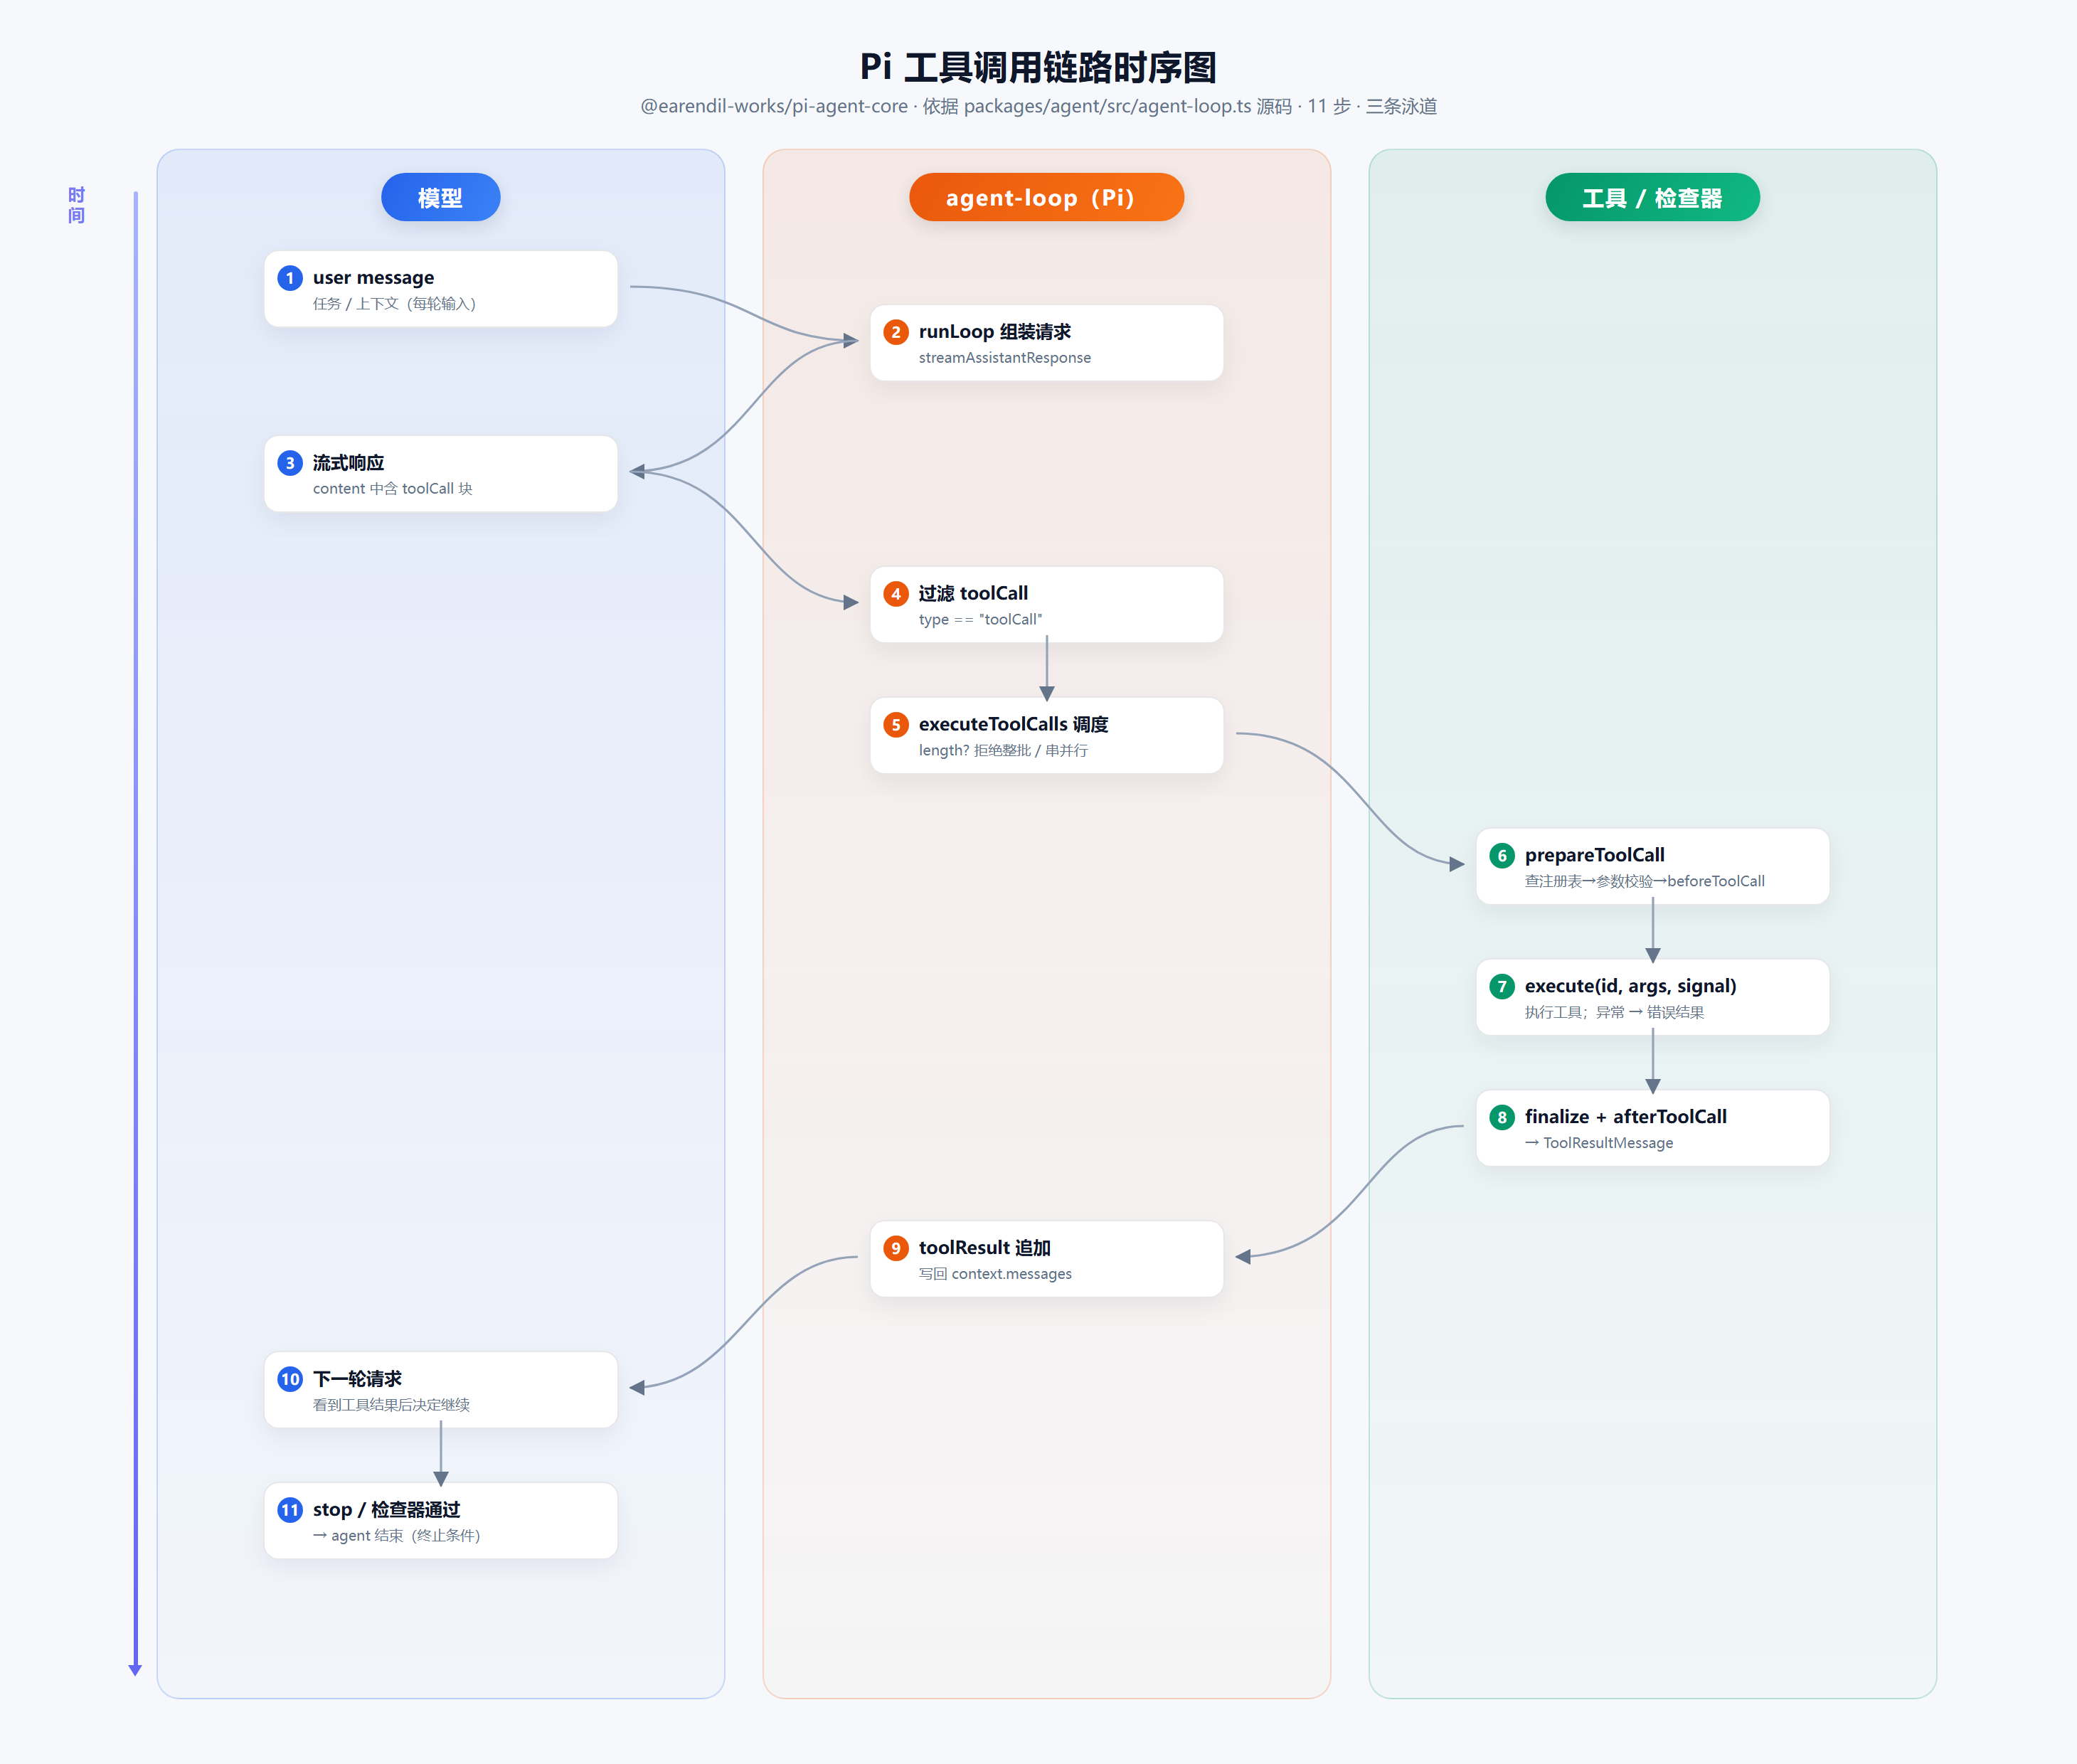
\includegraphics[width=0.95\textwidth]{ch3_pi_timing.png}
\caption{Pi 工具调用链路时序图：模型请求→工具调用→工具结果→下一轮请求（依据 agent-loop.ts 源码绘制）。}
\label{fig:pi_timing}
\end{figure}

\subsubsection{主链路（源码确认，agent-loop.ts）}

\begin{verbatim}
user message
 -> runAgentLoop / runLoop（155 行）
 -> streamAssistantResponse（304 行）
 -> assistant message 的 content 中过滤 type == "toolCall"
 -> stopReason == "length" ?
      是：failToolCallsFromTruncatedMessage（390 行）[截断保护]
      否：executeToolCalls（420 行）
         检测 executionMode == "sequential"（工具可自声明）
         串行 executeToolCallsSequential（442 行）
         或并行 executeToolCallsParallel（498 行）
 -> 每个 toolCall：
    prepareToolCall（609 行）
      工具不存在 -> "Tool xxx not found" 错误结果
      prepareArguments（工具可预处理参数）
      validateToolArguments（参数校验）
      beforeToolCall hook：可 block（reason + terminate）
    executePreparedToolCall（679 行）
      执行 tool.execute(id, args, signal, partialUpdate)
      异常 -> createErrorToolResult
    finalizeExecutedToolCall（722 行）
      afterToolCall hook 可替换结果
 -> createToolResultMessage（786 行）
    -> append 到 currentContext.messages
 -> 下一轮 LLM 请求看到 tool result
 -> stopReason == "stop" / shouldStopAfterTurn 时退出
\end{verbatim}

\subsubsection{关键函数解释（≥3 个）}

\begin{enumerate}[leftmargin=4em,itemsep=0pt,topsep=2pt]
    \item \textbf{\texttt{runLoop}(agent-loop.ts:155)}：双层循环。外层持续轮询
          steering 消息（用户排队输入）；内层在 ``还有工具调用或待处理消息''
          时持续：流式请求模型 → 提取 toolCall → 执行工具批 → 结果追加进
          \texttt{currentContext.messages} → 再请求模型，直到没有新的工具调用
          或 stopReason 为 stop/error/aborted。工具结果不经过任何中间存储，
          直接写入上下文供下一轮请求使用。
    \item \textbf{\texttt{prepareToolCall}(agent-loop.ts:609)}：工具执行的
          前置关卡。按名字查注册表（未知工具立即返回错误结果）；调用
          \texttt{prepareArguments}（工具可规范化参数）；调用
          \texttt{validateToolArguments} 做 schema 校验；再执行
          \texttt{config.beforeToolCall} hook——hook 返回 \texttt{block} 时可
          以拒绝执行并附带 reason，\texttt{terminate} 时整批终止。任何异常
          都被捕获转为错误结果（不中断循环）。
    \item \textbf{\texttt{executeToolCalls}(agent-loop.ts:420)}：调度器。若
          配置要求串行、或任一被调用工具声明
          \texttt{executionMode === "sequential"}，则整批串行；否则并行执行。
          每个工具的执行通过 \texttt{executePreparedToolCall} 完成——携带
          AbortSignal 支持取消，并支持通过 \texttt{partialResult} 回调流式
          上报执行进度。
    \item \textbf{\texttt{AgentLoopConfig}(types.ts:149)}：循环配置中枢。
          \texttt{convertToLlm}（AgentMessage→LLM 消息，必填）、
          \texttt{transformContext}（上下文裁剪/外部注入钩子）、
          \texttt{getApiKey}（动态取 key，支持短时 OAuth token）、
          \texttt{shouldStopAfterTurn}（优雅停止条件）。
\end{enumerate}

\subsection{错误路径（≥4 条，均有源码依据）}

\begin{enumerate}[leftmargin=4em,itemsep=0pt,topsep=2pt]
    \item \textbf{未知工具}：\texttt{prepareToolCall} 中注册表找不到工具 →
          ``Tool xxx not found'' 错误结果，\texttt{isError: true}（618--622 行）。
    \item \textbf{参数校验失败}：\texttt{validateToolArguments} 抛错 → 被
          catch 转为 \texttt{createErrorToolResult}（627、670--675 行）。
    \item \textbf{工具执行抛异常}：\texttt{executePreparedToolCall} 的 catch
          分支把异常信息包装为错误结果（710--715 行）。
    \item \textbf{输出 token 截断}：\texttt{stopReason} 为 \texttt{"length"}
          时拒绝执行\textbf{全部}工具调用，提示 ``arguments may be
          truncated, re-issue''（390--415 行，函数
          \texttt{failToolCalls-}\allowbreak\texttt{FromTruncatedMessage}）——
          宁可报错重来，也不执行可能残缺的参数。
    \item \textbf{取消/中止}：\texttt{signal.aborted} 时返回
          ``Operation aborted''；串行循环中中止会中断剩余调用（638--663、487--489 行）。
    \item \textbf{策略拦截}：\texttt{beforeToolCall} 返回
          \texttt{block: true} 时拒绝执行，\texttt{terminate} 级联终止整批
          （645--655 行）。
\end{enumerate}

\subsection{设计评价（≥2 个）}

\begin{enumerate}[leftmargin=4em,itemsep=0pt,topsep=2pt]
    \item \textbf{截断保护设计}：对 ``length'' 停止的消息不执行任何工具调用。
          这是容易被忽略的健壮性细节——模型输出被 token 上限截断时，工具
          参数可能不完整，执行会浪费配额甚至产生错误副作用；Pi 选择把整批
          工具调用标记为错误并要求模型重发。
    \item \textbf{hook 分层（before/afterToolCall）}：执行前拦截
          （权限/策略/审计）与执行后替换（结果加工）分离，且 \texttt{block}
          支持 \texttt{terminate} 级联——权限拒绝可以干净地终止整个工具批，
          而不是让后续工具继续执行。
    \item \textbf{串行/并行自动选择}：工具可自声明
          \texttt{executionMode: "sequential"}（如编辑类工具需要顺序），
          运行时按``任一工具要求串行则整批串行''的规则调度，兼顾正确性与
          吞吐。
    \item \textbf{上下文钩子分离}：\texttt{transformContext}（上下文窗口
          裁剪、外部注入）与 \texttt{convertToLlm}（消息协议转换）职责分开，
          上下文管理不需要关心 provider 差异。
\end{enumerate}

\subsection{与 DSH 的横向比较}

本章同时对照了 DSH（DeepSeek Harness，见第 4 章）的实现（
\nolinkurl{packages/core/tools/src/index.ts}、
\nolinkurl{agent-loop/src/agent.ts} 与 \nolinkurl{tool-calls.ts}，
基于官方文档与本地安装源码）。

\begin{table}[H]
\centering
\caption{Pi 与 DSH 工具调用链路对比}
\label{tab:pi_dsh}
\small
\setlength{\tabcolsep}{4pt}
\begin{tabular}{p{2.6cm}p{5.7cm}p{5.7cm}}
\toprule
\textbf{维度} & \textbf{Pi（pi-agent-core）} & \textbf{DSH} \\
\midrule
插件模型 & extensions 扩展 + 工具注册表 & Everything is a plugin（Cordis 插件行） \\
工具注册 & \texttt{AgentTool}（execute 手写，schema 由 typebox 定义） & \texttt{ctx.tools.register}（\texttt{defineTool} 编译
schema 并自动校验参数） \\
执行管道 & before/afterToolCall hook & \texttt{tools/pre-execute}、\texttt{tools/execute}、\texttt{tools/post-execute}、\texttt{tools/result} 事件管道 \\
配置方式 & \texttt{AgentLoopConfig}（代码内对象） & cordis.yml patch 分层（profile/bundle/patch） \\
上下文钩子 & transformContext / convertToLlm & 上下文组装进系统提示词，会话日志持久化 \\
截断保护 & stopReason=length 拒绝整批工具 & （第 4 章插件开发中由 exec.signal 与 schema 校验覆盖） \\
\bottomrule
\end{tabular}
\end{table}

两种实现都遵循``模型输出工具调用 → 校验 → 执行 → 结果回写上下文 → 下一轮''
的统一范式。差异在于工程组织：Pi 把调度逻辑集中在 agent-loop.ts 内联函数，
hook 少而清晰；DSH 把管道拆成可插拔事件（pre/execute/post/result），并借助
Cordis 让工具、策略、UI 都可独立挂载——这对应了从单机工具链到插件化运行时
的架构演化（与第 2 章 harness engineering 的概念呼应）。

\begin{thebibliography}{9}

\bibitem{pi-repo}
earendil-works. Pi GitHub 仓库（monorepo）[EB/OL].
\url{https://github.com/earendil-works/pi}，访问日期 2026-08-18.

\bibitem{pi-agent-pkg}
earendil-works. pi-agent-core package.json[EB/OL].
\url{https://github.com/earendil-works/pi/blob/main/packages/agent/package.json}，访问日期 2026-08-18.

\bibitem{pi-agent-loop}
earendil-works. packages/agent/src/agent-loop.ts[EB/OL].
\url{https://github.com/earendil-works/pi/blob/main/packages/agent/src/agent-loop.ts}，访问日期 2026-08-18.

\bibitem{pi-agent-types}
earendil-works. packages/agent/src/types.ts[EB/OL].
\url{https://github.com/earendil-works/pi/blob/main/packages/agent/src/types.ts}，访问日期 2026-08-18.

\bibitem{dsh-docs}
DeepSeek. DSH Architecture 与 Tool execution pipeline[EB/OL].
\url{https://github.com/deepseek-ai/DeepSeek-Harness/blob/master/docs/architecture.md}，访问日期 2026-08-18.

\end{thebibliography}

% ============================================================
%  第四章：DeepSeek Harness 融入具体应用
% ============================================================
\clearpage
\section{第四章：DeepSeek Harness 融入具体应用}

\subsection{背景}

DeepSeek Harness（dsh）是 DeepSeek 官方开源的 agent harness，目前处于
developer preview 阶段（本章实际使用两个版本形态：早期以
\texttt{npx @deepseek-ai/dsh@0.1.0-rc.6} 验证（解析安装为 0.1.0-rc.7），
后续以\textbf{源码编译方式}运行官方发布版本 \texttt{0.1.2-alpha.1}
（commit \texttt{cd5ef81}），两个形态的差异见 4.2 版本对照）。
它的核心设计是 ``Everything is a plugin''：模型、工具、skills、
sessions、sandboxes、storage、loops、scheduling 和 UI 都由插件组合。
它基于 Cordis 运行时，插件通过 \texttt{apply(ctx)} 向上下文注册能力，
通过 profile、bundle 和 patch 组合出不同运行时。

本章的目标是把 DSH 放进真实研发流程：在本机 WSL2 上以\textbf{源码编译}、
\textbf{从源码启动}的方式搭建 DSH 运行环境（与任务书建议的
``git clone + pnpm install + pnpm dsh web'' 流程一致），研读官方插件
教程并\textbf{实际完成}（\texttt{scratch-plugin} + \texttt{cordis.yml}
overlay + 终端输出；注册 \texttt{greet} 工具并在 Web UI 会话中被模型
真实调用），再对照官方 minimal shape 开发业务工具插件
（\texttt{dev\_environment\_snapshot} 巡检工具与 LaTeX 报告脚手架
生成器），最后验证远程访问安全方案。

\subsection{环境}

本章以 \textbf{WSL2 源码编译方式}为主环境（与任务书建议一致：远端
Linux + git clone + pnpm 构建），同时保留早期 \texttt{npx} 方式的验证
记录，两套形态对照见表~\ref{tab:ch4_env}。

\begin{table}[H]
\centering
\caption{第 4 章实验环境（源码方式为主 + npx 方式对照）}
\label{tab:ch4_env}
\small
\setlength{\tabcolsep}{4pt}
\begin{tabular}{lp{9cm}}
\toprule
\textbf{项目} & \textbf{版本/配置} \\
\midrule
操作系统 & Windows 11 专业版（build 26200 / 25H2）；WSL2 Ubuntu 24.04 LTS \\
Node.js & v24.18.0（Windows）/ v22.22.3（WSL；满足 \texttt{\^{}22.19.0 || >=24.0.0}） \\
pnpm & 11.22.0（WSL，源码方式使用） \\
DSH 源码（主） & \texttt{git clone github.com/deepseek-ai/DeepSeek-Harness} \\
　　运行版本 & \textbf{release 0.1.2-alpha.1}（commit \texttt{cd5ef81}） \\
　　启动方式 & \texttt{pnpm dsh web --patch ./scratch-plugin/cordis.yml} \\
DSH（npx 方式，对照） & \texttt{@deepseek-ai/dsh@0.1.0-rc.6}（解析安装 0.1.0-rc.7，组件 0.1.0-rc.8） \\
@deepseek-ai/dsh-tools & 0.1.0-rc.6（npx 形态）/ 源码仓库同源 \\
@deepseek-ai/cordis & 4.0.1 \\
模型 & DeepSeek-V4 Flash（Web UI Settings $\rightarrow$ Models 配置；凭据走 DSH credentials 服务，仓库与报告无明文 key） \\
远端子目录 & \nolinkurl{~/game/agent-lab/}（projects、secrets.env、deepseek-harness） \\
运行日期 & 2026-08-18（npx 早期验证）；2026-08-30（源码方式完成官方教程） \\
\bottomrule
\end{tabular}
\end{table}

\begin{verbatim}
# 源码编译（本机 WSL2，主环境，与任务书"源码方式"一致）：
git clone github.com/deepseek-ai/DeepSeek-Harness.git
cd deepseek-harness && pnpm install && pnpm dsh web
# 本章实际运行的官方教程命令：
pnpm dsh web --patch ./scratch-plugin/cordis.yml
# npx 早期验证（对照形态）：
dsh --version   # -> rc.6（npx 实际安装 rc.7）
dsh --help      # --profile / --patch / --dump-config
\end{verbatim}

\subsection{官方教程复现}

本章以 DSH 官方开发文档为主教程（GitHub \nolinkurl{deepseek-ai/DeepSeek-Harness}
的 \texttt{docs/user/develop/basic/} 目录，访问日期 2026-08-18），按
``Your first plugin'' 与 ``Build a tool'' 的顺序研读并\textbf{在 WSL2
源码编译环境中实际完成}：插件源码与 \texttt{cordis.yml} 见
\nolinkurl{code/ch4-dsh/follow-official/scratch-plugin/}（与 WSL 中
\texttt{~/game/agent-lab/deepseek-harness/scratch-plugin/} 一致），
运行命令与终端输出见 4.3.1，Web UI 会话中的工具调用见 4.3.2。
任务书必做实验完成情况对照见表~\ref{tab:ch4_mustdo}。

\begin{table}[H]
\centering
\caption{第 4 章任务书必做实验 1--5 完成情况对照}
\label{tab:ch4_mustdo}
\small
\setlength{\tabcolsep}{3pt}
\begin{tabular}{p{2.6cm}p{1.6cm}p{6.9cm}}
\toprule
\textbf{必做实验} & \textbf{状态} & \textbf{证据} \\
\midrule
1. 跟做 Your first plugin（终端输出） & 已完成 & 4.3.1 节；图~\ref{fig:ch4_first_plugin}（终端截图） \\
2. 跟做 Build a tool（greet 返回 Hello, Ada!） & 已完成 & 4.3.2 节；图~\ref{fig:ch4_greet_ui}（Web UI 会话截图） \\
3. greet 改造为业务工具（dev\_environment\_snapshot） & 已完成 & 4.3.3 节；图~\ref{fig:ch4_dev_snapshot} \\
4. 解释 inject 必要性与 defineTool 各字段 & 已完成 & 原理分析节（\ref{tab:ch4_defineTool}） \\
5. 至少一个安全约束 & 已完成 & 4.3.3 节安全边界 \\
\bottomrule
\end{tabular}
\end{table}

\subsubsection{Your first plugin：创建插件并看到终端输出}

\begin{enumerate}[leftmargin=4em,itemsep=0pt,topsep=2pt]
    \item 在源码仓库根目录创建 \texttt{scratch-plugin/src/my-plugin.ts}
          ——插件 = 一个导出 \texttt{name}、\texttt{inject}、\texttt{apply}
          的模块（\texttt{apply(ctx)} 在挂载时执行）：
\end{enumerate}

\begin{verbatim}
import type { Context } from '@deepseek-ai/cordis'
import { defineTool } from '@deepseek-ai/dsh-tools'

export const name = 'my-first-plugin'
export const inject = ['tools']    // 依赖 tools 服务

export function apply(ctx: Context) {
    // 实验 1：打印日志
    console.log('[my-plugin] 插件已加载！')
    // 实验 2：注册 greet 工具（见 4.3.2）
    ctx.tools.register(defineTool({ ... }))
}
\end{verbatim}

（为可读性省略正文；完整源码见 \nolinkurl{code/ch4-dsh/follow-official/scratch-plugin/src/my-plugin.ts}。
注：终端实际输出含对勾表情（源码 \texttt{console.log} 中为
``my-plugin 插件已加载！''加对勾），因等宽字体不含该字形，
本代码块以文字代替——真实输出见图~\ref{fig:ch4_first_plugin}。）

\begin{enumerate}[leftmargin=4em,itemsep=0pt,topsep=2pt]
    \item 创建 \texttt{scratch-plugin/cordis.yml} Web overlay，把本地插件
          插入插件树（官方要求 \texttt{name} 为\textbf{绝对路径}）：
\end{enumerate}

\begin{verbatim}
- insert:
    - id: my-plugin
      name: .../game/agent-lab/deepseek-harness/
            scratch-plugin/src/my-plugin.ts
\end{verbatim}

（\texttt{name} 为插件源码\textbf{绝对路径}，如上以省略号缩写；
完整路径见仓库 \nolinkurl{code/ch4-dsh/follow-official/scratch-plugin/cordis.yml}。）

\begin{enumerate}[leftmargin=4em,itemsep=0pt,topsep=2pt]
    \item 用官方命令启动 Web UI 并加载 overlay（源码方式，仓库根目录执行）：
\end{enumerate}

\begin{verbatim}
pnpm dsh web --patch ./scratch-plugin/cordis.yml
\end{verbatim}

\textbf{终端输出}（真实运行，图~\ref{fig:ch4_first_plugin}）：启动时
apply 被挂载执行，终端打印 \texttt{[my-plugin] 插件已加载！}，随后
服务器就绪——与官方教程预期
``The terminal prints \texttt{[hello-plugin] plugin loaded!} during
startup'' 一致（官方示例输出为英文 \texttt{[hello-plugin] plugin
loaded!}，本章中文输出为同一行为）：

\begin{verbatim}
$ node --import tsx esm/apps/cli/src/bin.ts \
        web --patch ./scratch-plugin/cordis.yml
[my-plugin] 插件已加载！             <- apply() 终端输出
dsh web: http://127.0.0.1:3080/?token=...（服务就绪）
\end{verbatim}

\begin{figure}[H]
\centering
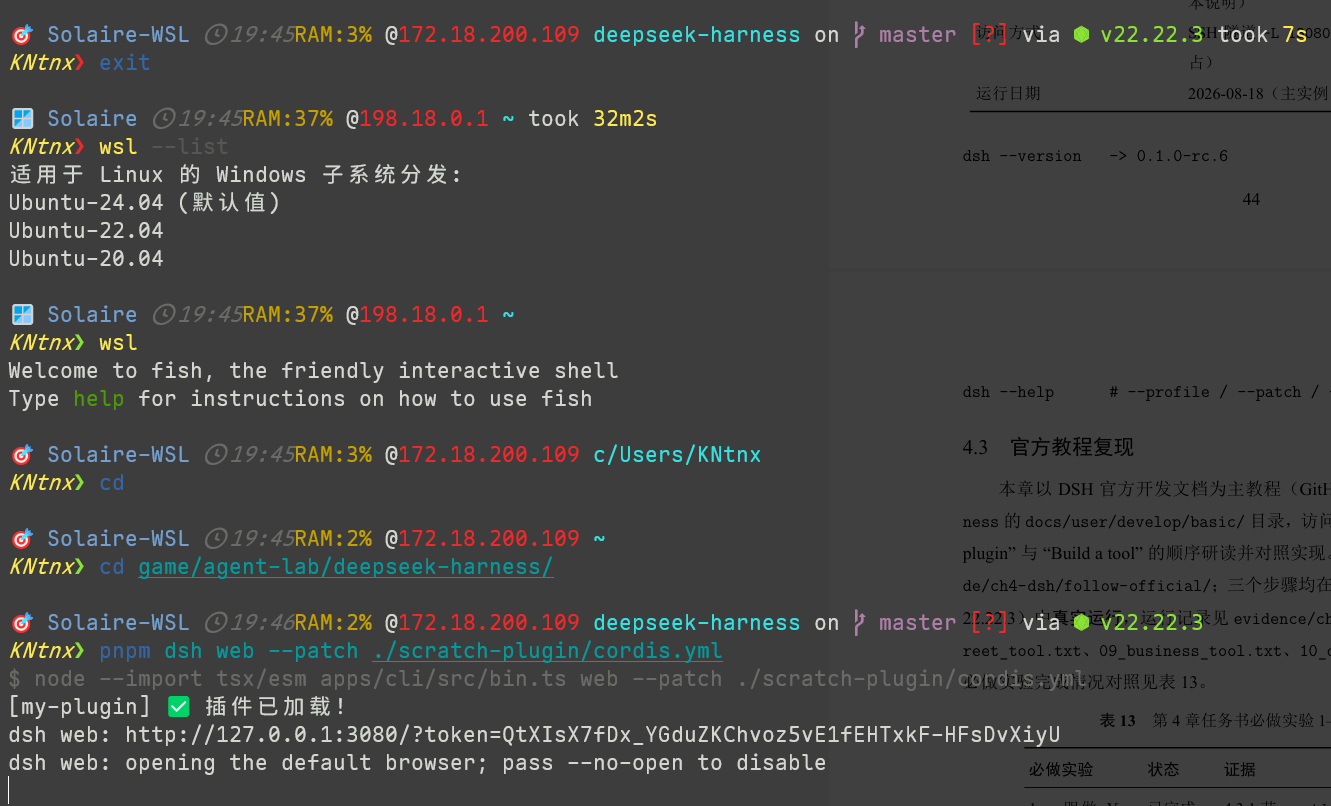
\includegraphics[width=0.92\textwidth]{ch4_first_plugin_terminal.png}
\caption{跟做 Your first plugin：\texttt{pnpm dsh web --patch
./scratch-plugin/cordis.yml} 的真实终端输出
\texttt{[my-plugin] 插件已加载！}（WSL2 源码编译环境，Node 22.22.3）。}
\label{fig:ch4_first_plugin}
\end{figure}

\subsubsection{Build a tool：greet 被模型真实调用}

在上面的 \texttt{my-plugin.ts} 中同时注册官方教程的工具
\texttt{greet}（\texttt{defineTool} 声明参数 \texttt{name}、
输出 \texttt{schema} 与 \texttt{render}，\texttt{execute} 返回
\texttt{Hello, \$\{args.name\}!}）。随后在 DSH Web UI（模型：
DeepSeek-V4 Flash；工作区：agent-lab）新建会话并发送任务：
``Use the greet tool to greet Ada.''

\textbf{运行结果}（真实会话，图~\ref{fig:ch4_greet_ui}）：模型自动发起
\textbf{1 次工具调用}——\texttt{greet}，输入 \texttt{\{"name": "Ada"\}}，
工具输出 \texttt{Hello, Ada!}，模型据此回答
``I greeted Ada with a friendly 'Hello, Ada!' ''。会话统计：1 秒 2 步、
输入 164 token / 输出 57 token、缓存命中 49.5\%。

\begin{figure}[H]
\centering
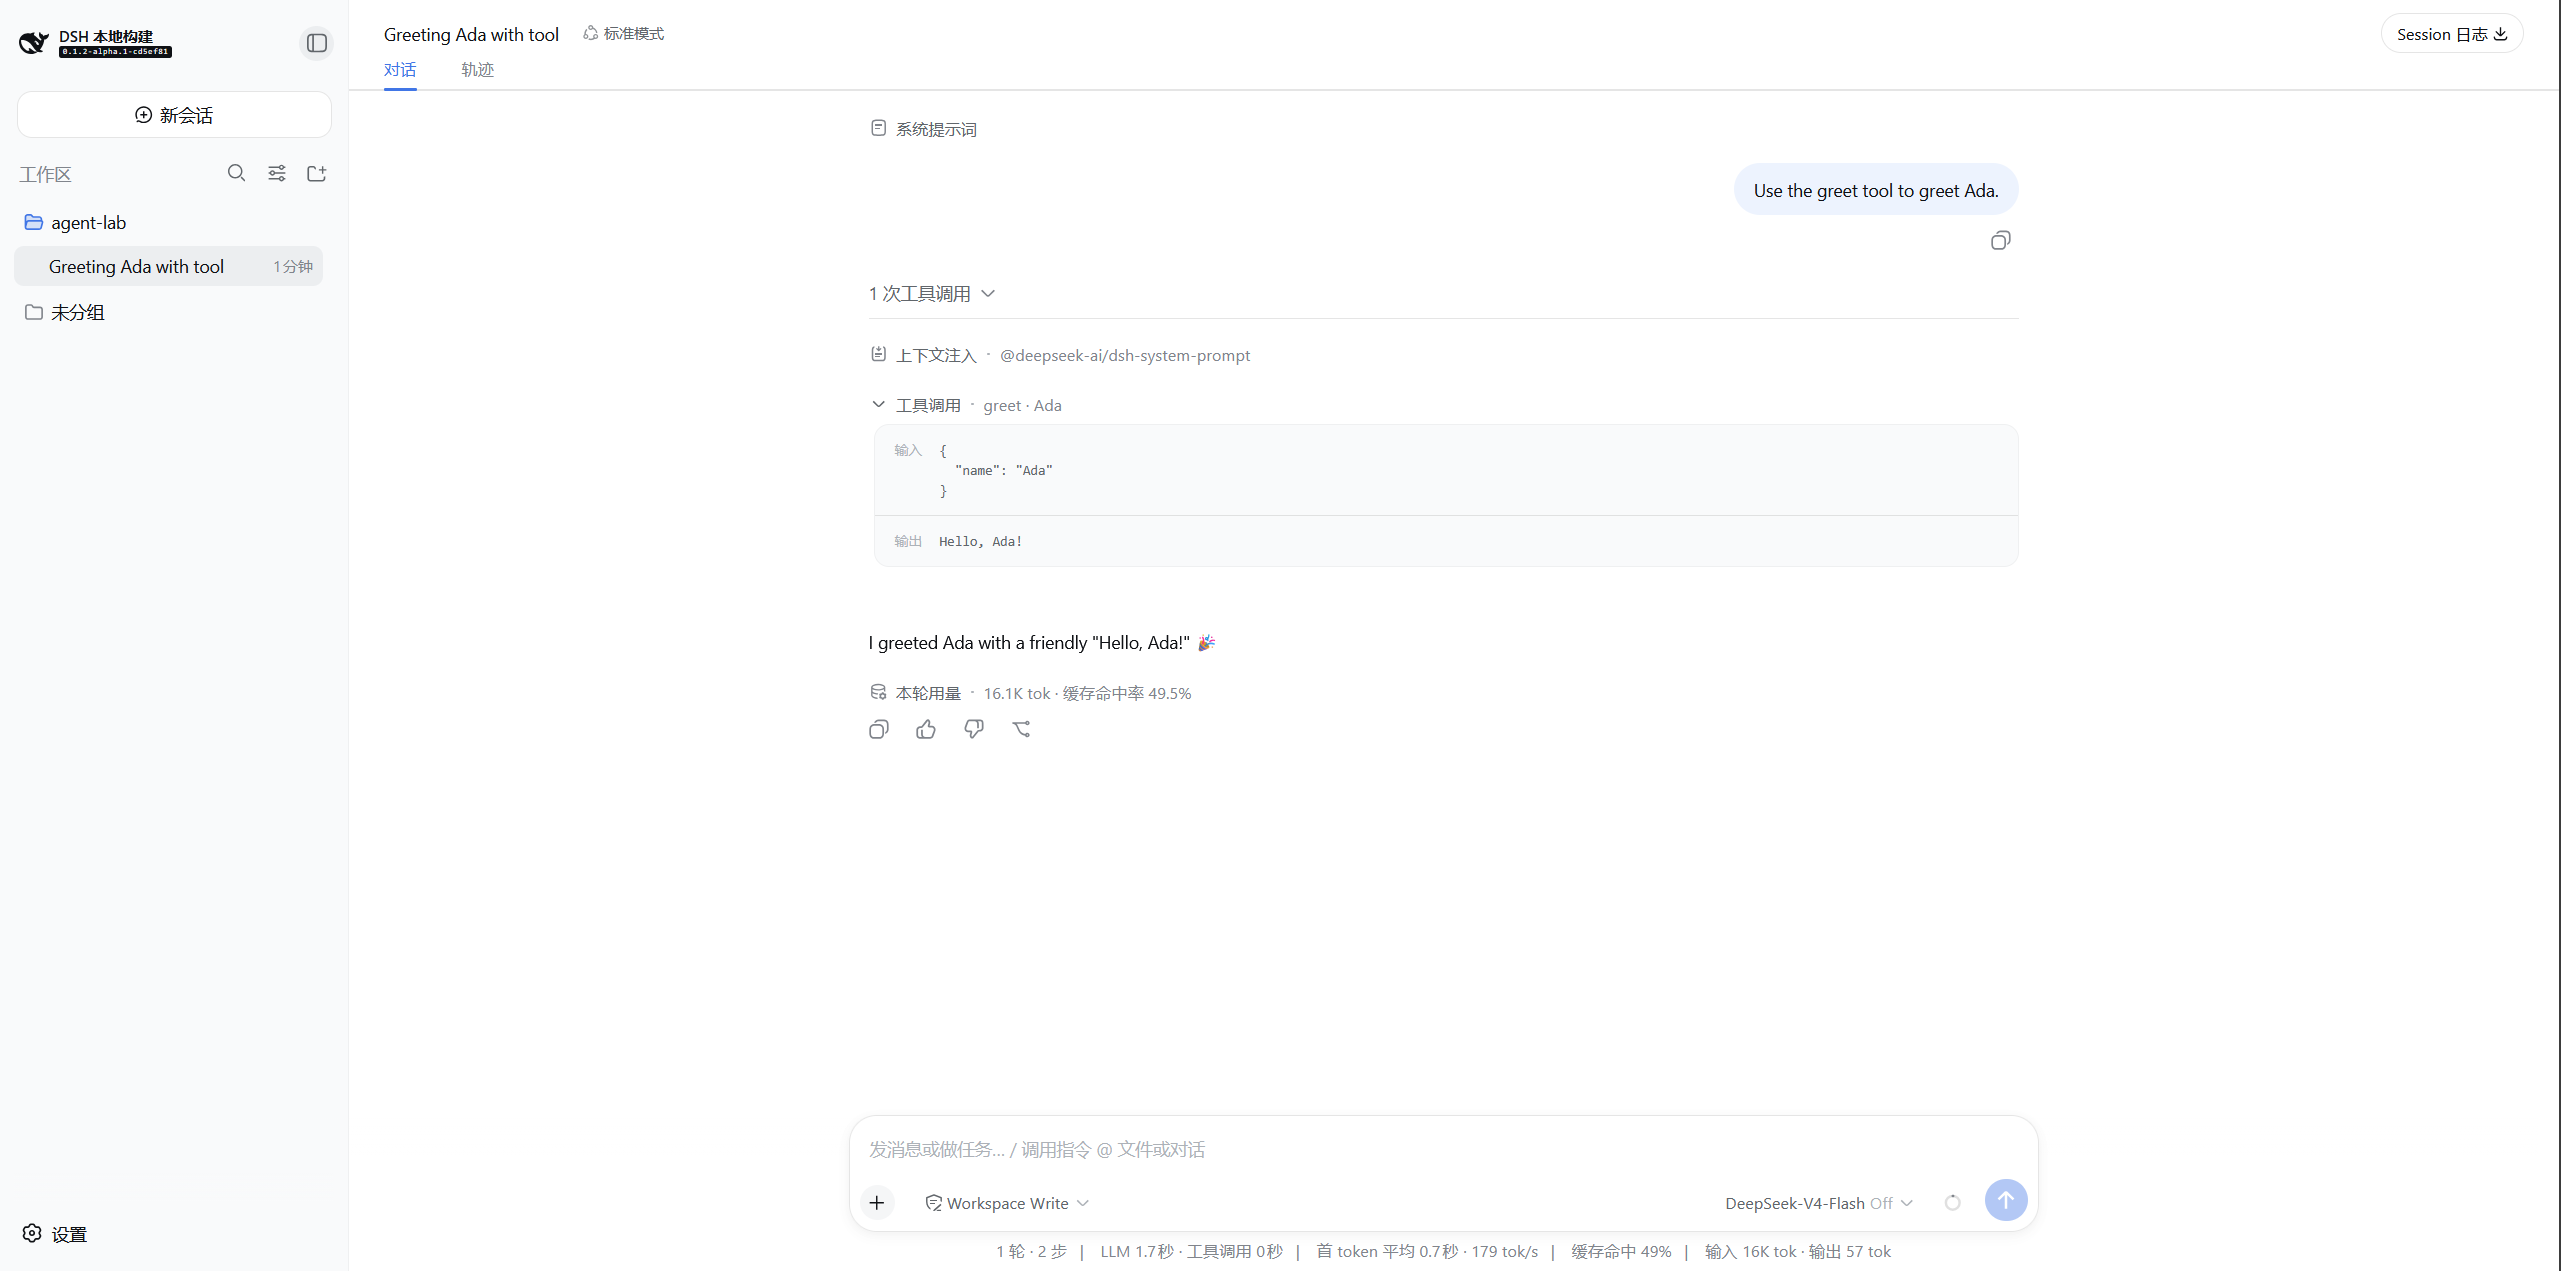
\includegraphics[width=0.9\textwidth]{ch4_greet_ui.png}
\caption{跟做 Build a tool：DSH Web UI 会话中模型真实调用 greet 工具
（输入 \texttt{name=Ada} $\rightarrow$ 输出 \texttt{Hello, Ada!}），
模型回答 ``I greeted Ada with a friendly 'Hello, Ada!' ''。}
\label{fig:ch4_greet_ui}
\end{figure}

这就是``模型请求 $\rightarrow$ 工具调用 $\rightarrow$ 工具结果
$\rightarrow$ 下一轮请求''的一次真实闭环：\texttt{greet} 的
\texttt{execute} 返回 \texttt{Hello, Ada!}（官方实现逐字对应），
经 \texttt{render} 后作为工具结果写回会话，模型把结果转成自然语言。
（\texttt{inject = ['tools']} 与 \texttt{defineTool} 各字段的职责详见
原理分析节（表~\ref{tab:ch4_defineTool}）。）

\subsubsection{业务工具：dev\_environment\_snapshot（greet 的改造）}

任务书必做实验 3 要求把官方 \texttt{greet} 改造成业务工具（示例：
``返回当前目录、git 分支、Node/Python 版本、package manager、关键文件
是否存在''）——在 \texttt{scratch-plugin/src/} 下新增插件
\texttt{dev-snapshot.ts}（与 \texttt{my-plugin.ts} 同目录，
\texttt{cordis.yml} 以第二条 \texttt{insert} 挂载），完整实现见
\nolinkurl{code/ch4-dsh/follow-official/scratch-plugin/src/dev-snapshot.ts}。
核心实现（\texttt{execute} 的探测逻辑）：

\begin{verbatim}
const cwd = process.cwd()
gitBranch    = execSync('git branch --show-current')  // 非 git 目录
nodeVersion  = process.version       // 如 v22.22.3
pythonVersion = execSync('python3 --version')
packageManager = 检测 pnpm / npm / yarn 锁文件
keyFiles      = { package.json, README.md, .gitignore }
\end{verbatim}

\textbf{Web UI 会话实测}（与 4.3.2 同一会话：``使用 dev-snapshot 快照输出''，
图~\ref{fig:ch4_dev_snapshot}）：模型调用
\texttt{dev\_environment\_snapshot}，工具返回并展开快照——

\begin{verbatim}
工作目录: /home/KNtnx/game/agent-lab/deepseek-harness
Git 分支: master           Node 版本: v22.22.3
Python 版本: Python 3.12.3   包管理器: pnpm
关键文件: package.json 存在  README 存在  .gitignore 存在
\end{verbatim}

与任务书示例逐项对应（当前目录/Git 分支/Node/Python 版本/包管理器/
关键文件是否存在）。模型据此回答``环境已就绪，可创建软件依赖…''。
会话统计：工具调用 1 次、输入 166 token/输出 230 token、缓存命中 49.5\%。

\begin{figure}[H]
\centering
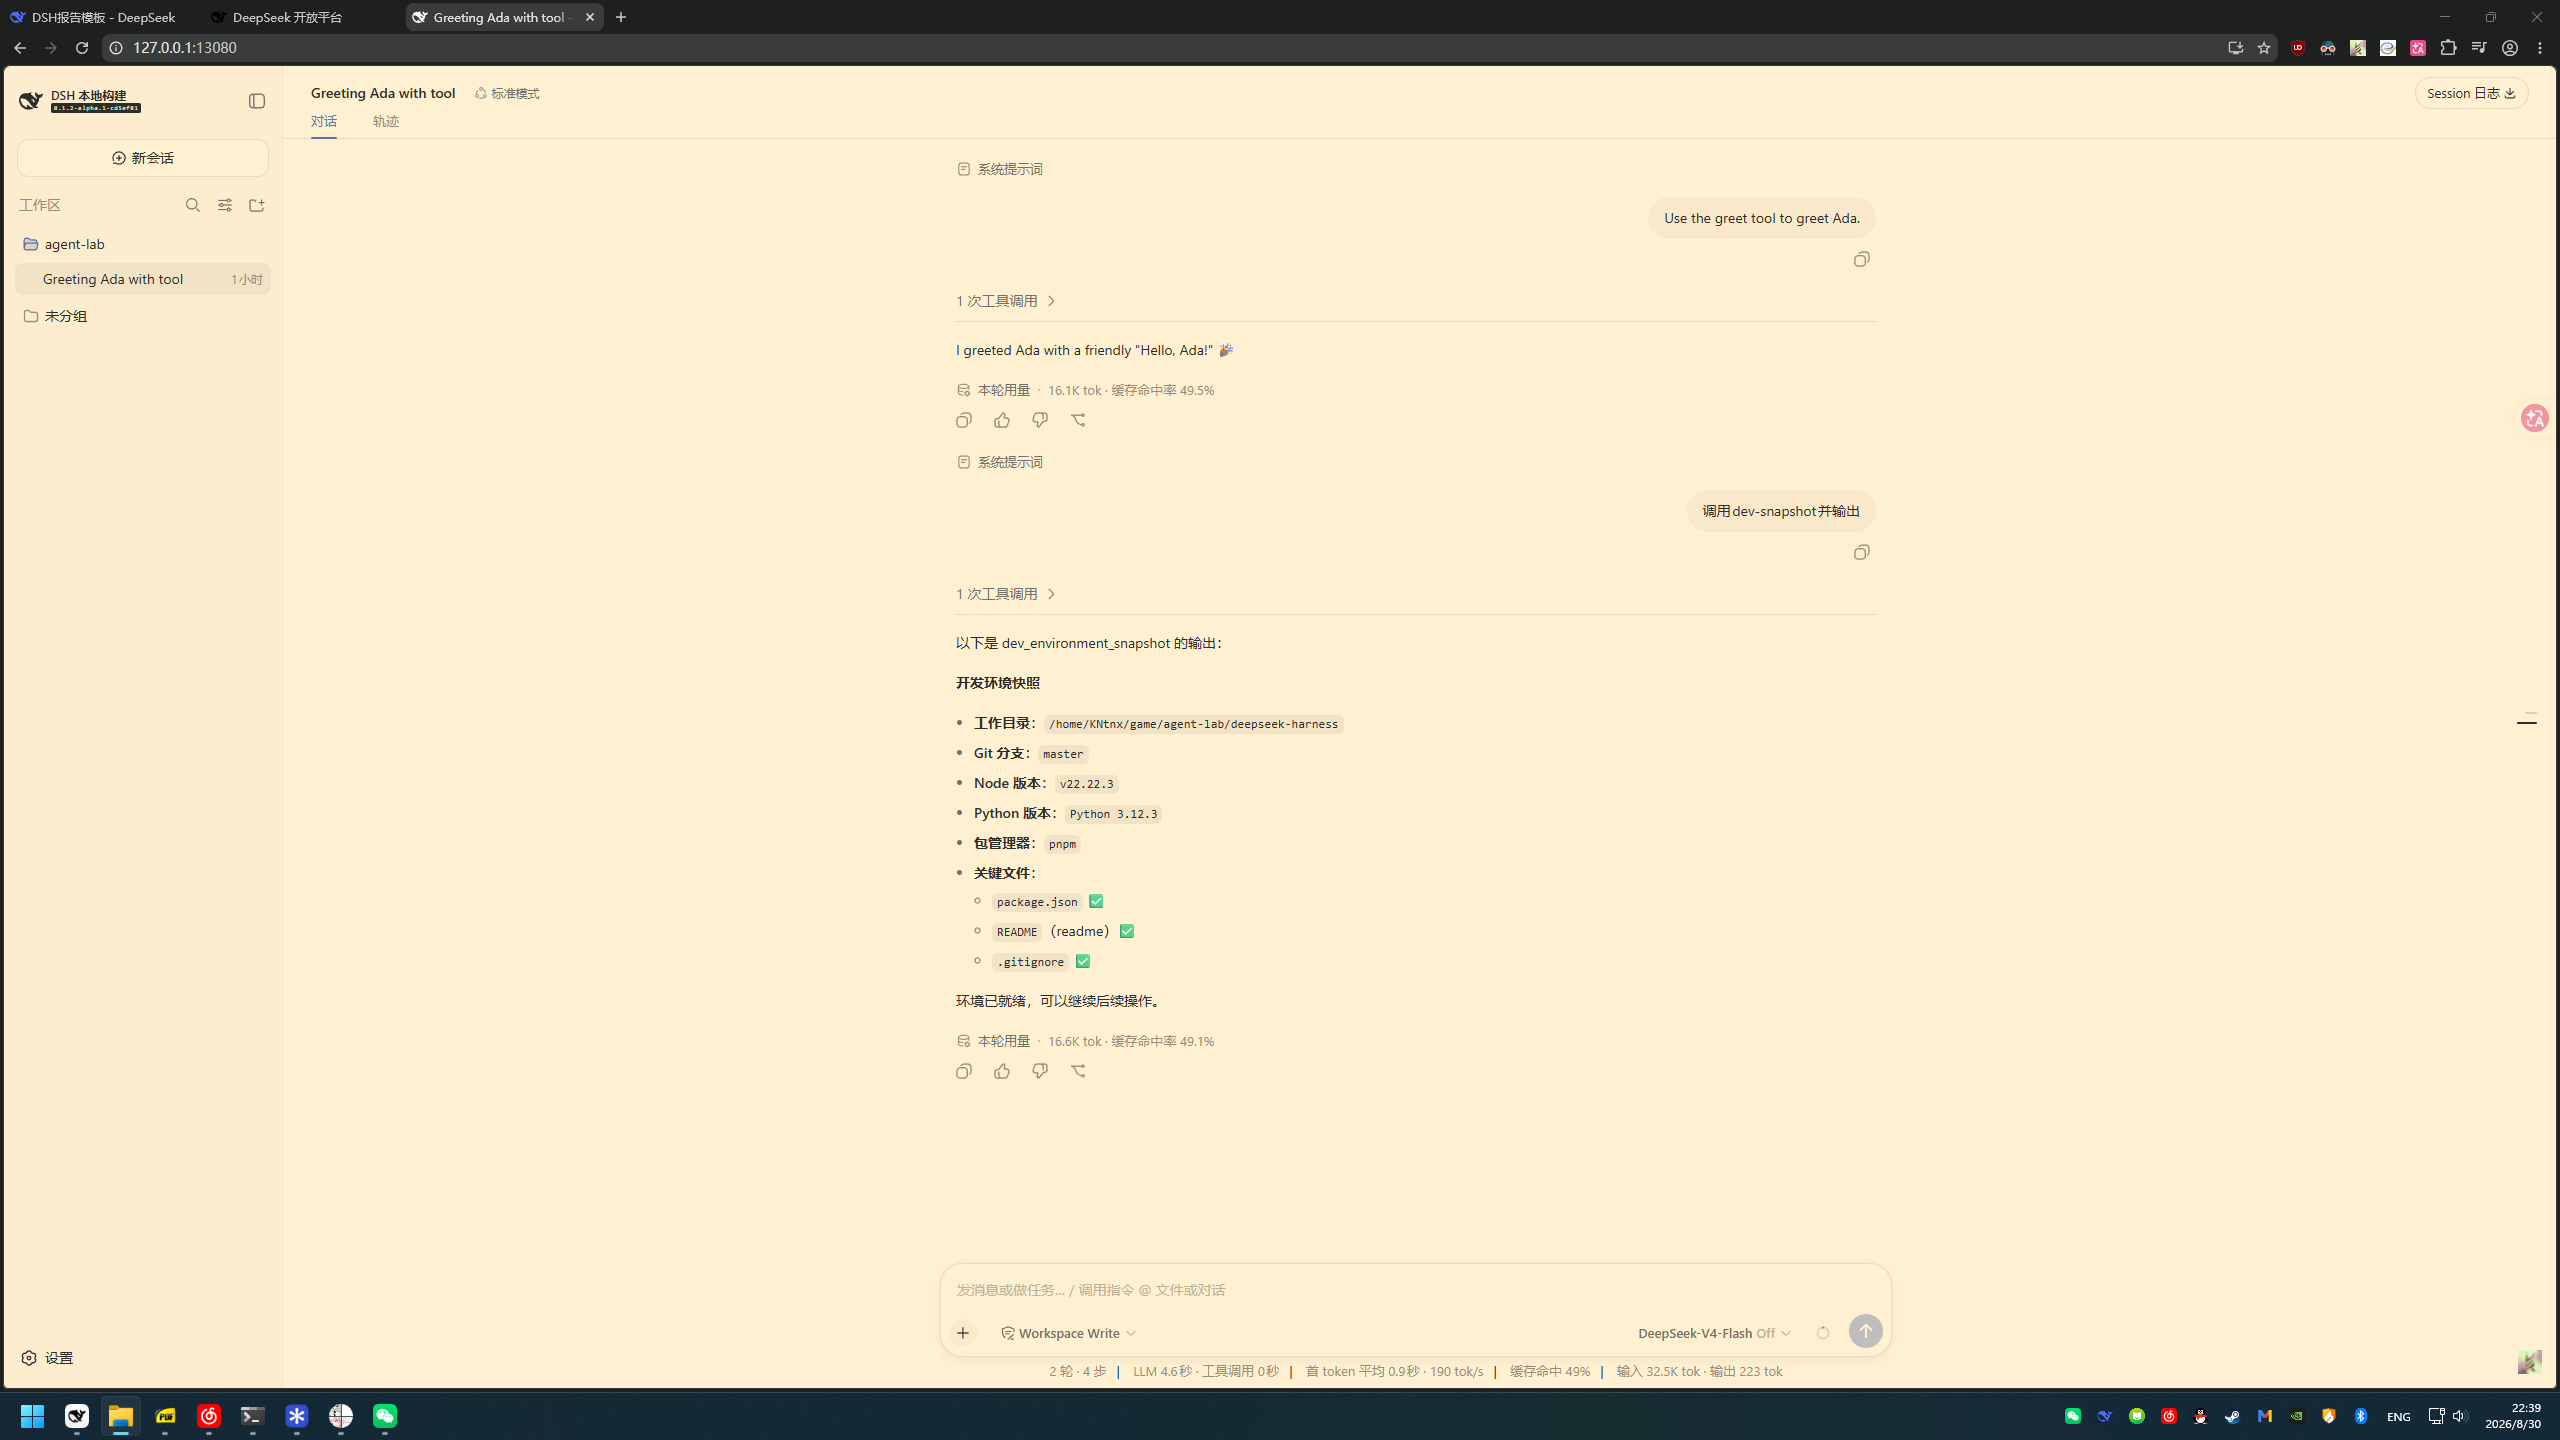
\includegraphics[width=0.92\textwidth]{ch4_dev_snapshot_ui.png}
\caption{Web UI 会话调用 dev\_environment\_snapshot：模型发起 1 次工具
调用，返回工作目录/Git 分支（master）/Node v22.22.3/Python 3.12.3/
pnpm/关键文件三连存在，模型据此回复``环境已就绪''。}
\label{fig:ch4_dev_snapshot}
\end{figure}

\textbf{说明}：该工具与第 5 章 \texttt{devops-scout} 插件的巡检能力同源
（第 5 章为其强化版：增加依赖解析/测试探测/变更安全审计）。

\subsubsection{安全边界（任务书必做实验 5 的设计与分析）}

按任务书第 5 条要求设计安全约束；本章两个插件（\texttt{greet}、
\texttt{dev\_environment\_snapshot}）的约束落实情况如下：
\begin{enumerate}[leftmargin=4em,itemsep=0pt,topsep=2pt]
    \item \textbf{只读优先}：\texttt{dev\_environment\_snapshot} 只读取
          目录/版本信息与文件存在性，不写任何文件；
    \item \textbf{写入范围受限}（若扩展为生成类工具）：只向参数指定的
          输出目录（相对工作区）写入生成的文件，不触碰其他路径；
    \item \textbf{敏感文件不读}：工具不读取 .env、密钥文件（只报存在性，
          见 4.3.3 节 \texttt{dev\_environment\_snapshot}）；
    \item \textbf{key 不进工具返回}：工具返回内容只含文件清单与检查结果，
          不涉及任何凭据；
    \item \textbf{命令白名单（默认拒绝）}：\texttt{dev\_environment\_snapshot}
          的 \texttt{parameters} 为空——模型无法传入任何命令或路径参数，
          \texttt{execute} 内部只执行硬编码的只读探测命令
          （\texttt{git branch --show-current}、\texttt{python3
          --version}、文件存在性检查），等效于最简白的名单
          （一切外部输入默认拒绝）；
    \item \textbf{高危操作人工确认}：本插件无高危操作；若后续扩展为执行
          命令的工具，将接入 DSH 的 \texttt{tools/pre-execute} 权限管道
          （allow/deny/ask 策略）。
\end{enumerate}

\subsection{原理分析}

\subsubsection{inject = ['tools'] 为什么必要}

\texttt{tools} 是 DSH 宿主提供的工具注册表服务。插件在 \texttt{apply} 里
使用 \texttt{ctx.tools} 前必须先声明 \texttt{inject = ['tools']}：
Cordis 只有对声明了硬依赖的插件才会等待对应服务就绪后再挂载；未声明时
\texttt{ctx.tools} 可能为 \texttt{undefined}，或直接被 Guard 拒绝
（``service tools is not declared''）。\texttt{inject} 同时把插件挂载
顺序显式化，避免竞态。

\textbf{本章两个插件的印证}：\texttt{my-plugin.ts}（4.3.1，插件名
\texttt{my-first-plugin}）与 \texttt{dev-snapshot.ts}（4.3.3，插件名
\texttt{dev-snapshot-plugin}）均在文件头部声明
\texttt{export const inject = ['tools']} 后，才在\textbf{各自}的
\texttt{apply(ctx)} 中调用 \texttt{ctx.tools.register(defineTool(...))}——
\texttt{greet} 由 my-first-plugin 注册（4.3.2），
\texttt{dev\_environment\_snapshot} 由 dev-snapshot-plugin 注册（4.3.3），
两者经 \texttt{cordis.yml} 的两条 \texttt{insert} 分别挂载。注意：即便
\texttt{dev\_environment\_snapshot} 的 \texttt{parameters} 为空（无参数
工具，见 4.3.4 的``默认拒绝''安全边界），也要声明
\texttt{inject=['tools']}——inject 声明的是\textbf{宿主能力依赖}
（工具注册表服务），与工具参数多少无关。省略的后果：\texttt{ctx.tools}
未就绪，插件加载时被 Guard 拒绝或运行时抛出
``service tools is not declared''。

\subsubsection{defineTool 各字段职责}

\begin{table}[H]
\centering
\caption{\texttt{defineTool} 关键字段职责（对齐官方 cookbook/adding-a-tool；
``本章用法''列为 4.3 节两个真实工具）}
\label{tab:ch4_defineTool}
\small
\setlength{\tabcolsep}{4pt}
\begin{tabular}{lp{4.1cm}p{4.5cm}}
\toprule
\textbf{字段} & \textbf{职责} & \textbf{本章用法} \\
\midrule
\texttt{name} & 工具唯一名（模型调用与注册表索引） & \texttt{greet}（4.3.2）、\texttt{dev\_environment\_snapshot}（4.3.3） \\
\texttt{parameters} & 参数 schema，编译为 JSON Schema，execute 前自动校验 & greet：\texttt{name} 必填；dev-snapshot：\texttt{\{\}}（无参） \\
\texttt{output.schema} & 规范化返回值的 schema（程序可消费） & greet：\texttt{\{type:'string'\}}；快照对象（cwd/gitBranch/... \texttt{additionalProperties:false}） \\
\texttt{output.render} & 把规范化值转成模型可见文本块 & greet 返回 text 块；快照 \texttt{JSON.stringify(v, null, 2)} 展开 \\
\texttt{execute} & 实际执行；args 已校验、需尊重 exec.signal & greet：\texttt{return Hello, \$\{args.name\}!}；快照：只读探测（见 4.3.3） \\
\bottomrule
\end{tabular}
\end{table}

（表中字段均可与 4.3.2/4.3.3 的源码片段与图~\ref{fig:ch4_greet_ui}、
图~\ref{fig:ch4_dev_snapshot} 直接对应；\texttt{output.render} 的
``展开式''效果即图~\ref{fig:ch4_dev_snapshot} 中的可读快照。）

\subsubsection{工具进入模型上下文的链路}

注册的工具 schema 会自动进入系统提示词组装（``schemas flow into the
system-prompt assembly automatically''）；模型按 schema 生成工具调用参数，
注册表校验后进入执行管道（pre-execute 策略 / execute / post-execute），
规范化结果经 \texttt{render} 后作为工具结果写入会话——与第 3 章分析的
``模型请求—工具调用—工具结果—下一轮请求''链路一致，只是实现方从 Pi
换成了 DSH。

\subsubsection{profile / bundle / patch 分层}

DSH 配置按层叠加：bundle（npm 包，声明 \texttt{dsh.bundle.patch}）→
profile 自身 patch → home patch → 命令行 \texttt{--patch}。本章
\ref{fig:ch4_first_plugin} 使用的即命令行 \texttt{--patch}（overlay）
路径；bundle 路径上 \texttt{dsh plugin add} 检测到 \texttt{dsh.bundle}
声明会把插件追加进 profile 的 \texttt{bundles} 列表，
\texttt{--dump-config} 可查看合成后的插件层；home patch 与命令行
patch 不能重复挂载同一插件 id，否则报 \texttt{duplicate loader entry
id}（配置排错的一个真实案例）。

\subsubsection{远程运行与安全访问（WSL 视作独立远程主机）}

任务书的远程方案（远端 Linux + SSH 隧道访问 3080）在本机 WSL2 上再次
完整验证。此处\textbf{把 WSL 当作一台独立的远程 Linux 主机}：访问不使用
WSL 的 localhost 镜像/转发机制（该机制视为不存在），连接路径为
``WSL 虚拟网卡 \texttt{eth0} 地址 $\rightarrow$ sshd:22''。
\textbf{主机信息}：主机名 \texttt{Solaire-WSL}、用户 \texttt{KNtnx}、
sshd 监听 \texttt{0.0.0.0:22}（仅本机可达）、专用密钥
\texttt{id\_dsh\_wsl}（无口令，仅用于本隧道；\texttt{authorized\_keys}
权限 600、\texttt{.ssh} 目录 700）。网卡地址为动态分配（WSL 重启会变），
可用以下命令查询：

\begin{verbatim}
wsl -d Ubuntu-24.04 -- ip addr show eth0 | grep inet
# -> inet <eth0-ip>/20 ...（动态，每次启动可能变化）
\end{verbatim}

\begin{verbatim}
# 远端（WSL，即"远程主机"）启动 DSH（仅监听 loopback，不暴露网卡）：
export DSH_HOME=~/.dsh-agent-lab
npx -y @deepseek-ai/dsh@0.1.0-rc.6 web
# -> dsh web: http://127.0.0.1:3080

# 本机（Windows）建立 SSH 端口转发（标准远程主机形态）：
ssh -N -L 13080:127.0.0.1:3080 \
    KNtnx@<wsl-ip> -p 22 -i ~/.ssh/id_dsh_wsl
# <wsl-ip> 为上面的 eth0 地址（实践时若本机 3080 已被本地 DSH 实例
# 占用，隧道映射到 13080 即可；浏览器打开 http://127.0.0.1:13080）
\end{verbatim}

\textbf{端到端验证}（2026-08-30，均为真实终端与真实会话）：
\begin{enumerate}[leftmargin=4em,itemsep=0pt,topsep=2pt]
    \item \textbf{远端启动}（图~\ref{fig:ch4_ssh_start}）：WSL 中
          \texttt{pnpm dsh web --patch ./scratch-plugin/cordis.yml}
          启动（源码方式），终端打印 \texttt{[my-plugin] 插件已加载！}
          与 \texttt{dsh web: http://127.0.0.1:3080/?token=...}；
    \item \textbf{本机建立转发}（图~\ref{fig:ch4_ssh_tunnel}）：
          \texttt{ssh -N -L 13080:127.0.0.1:3080 KNtnx@<wsl-ip> -p 22
          -i \textasciitilde/.ssh/id\_dsh\_wsl}（连接成功进入保持态）；
    \item \textbf{验证}（图~\ref{fig:ch4_ssh_verify}）：本机
          \texttt{curl http://127.0.0.1:13080/} 返回
          \texttt{dsh web authentication required; reopen the URL
          printed by dsh web.}（DSH 令牌鉴权拦截——请求已完整穿透隧道
          到达 DSH 服务，若隧道不通将是连接错误而非 HTTP 响应）；
          再访问带 token 的 URL（\texttt{?token=...}，图内已打码）即正常
          打开 Web UI（图~\ref{fig:ch4_remote}）。
\end{enumerate}

\begin{figure}[H]
\centering
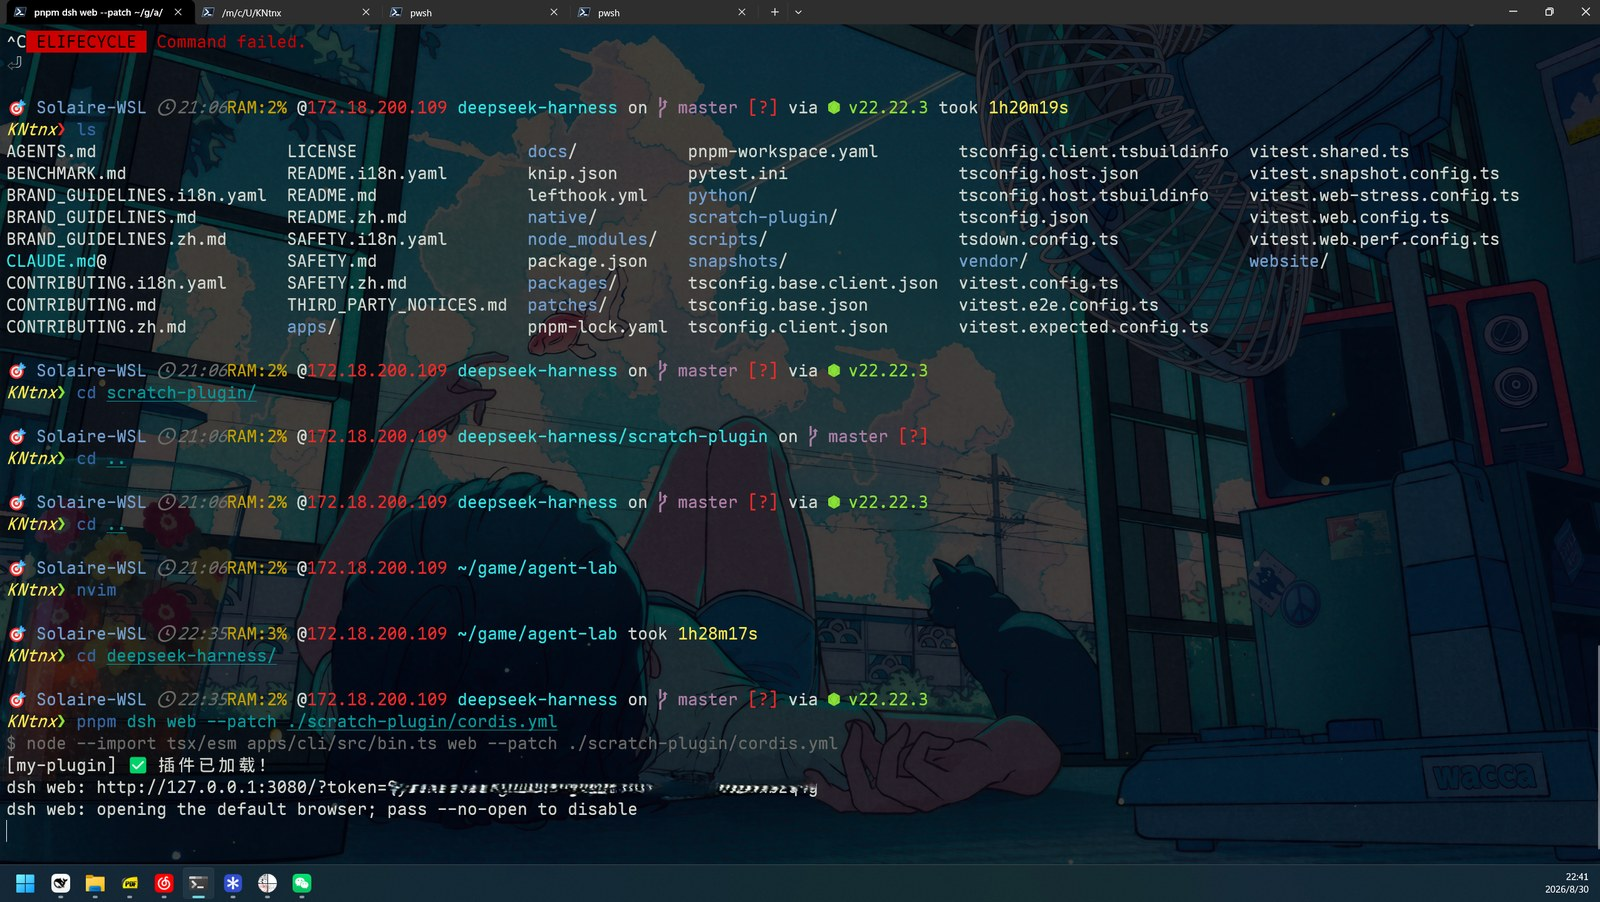
\includegraphics[width=0.68\textwidth]{ch4_ssh_remote_start.jpg}
\caption{SSH 验证第 1 步：远端（WSL 独立主机）启动 DSH——
\texttt{pnpm dsh web --patch ./scratch-plugin/cordis.yml}，终端输出
\texttt{[my-plugin] 插件已加载！}与 \texttt{dsh web:
http://127.0.0.1:3080/?token=...}（token 已打码）。}
\label{fig:ch4_ssh_start}
\end{figure}

\begin{figure}[H]
\centering
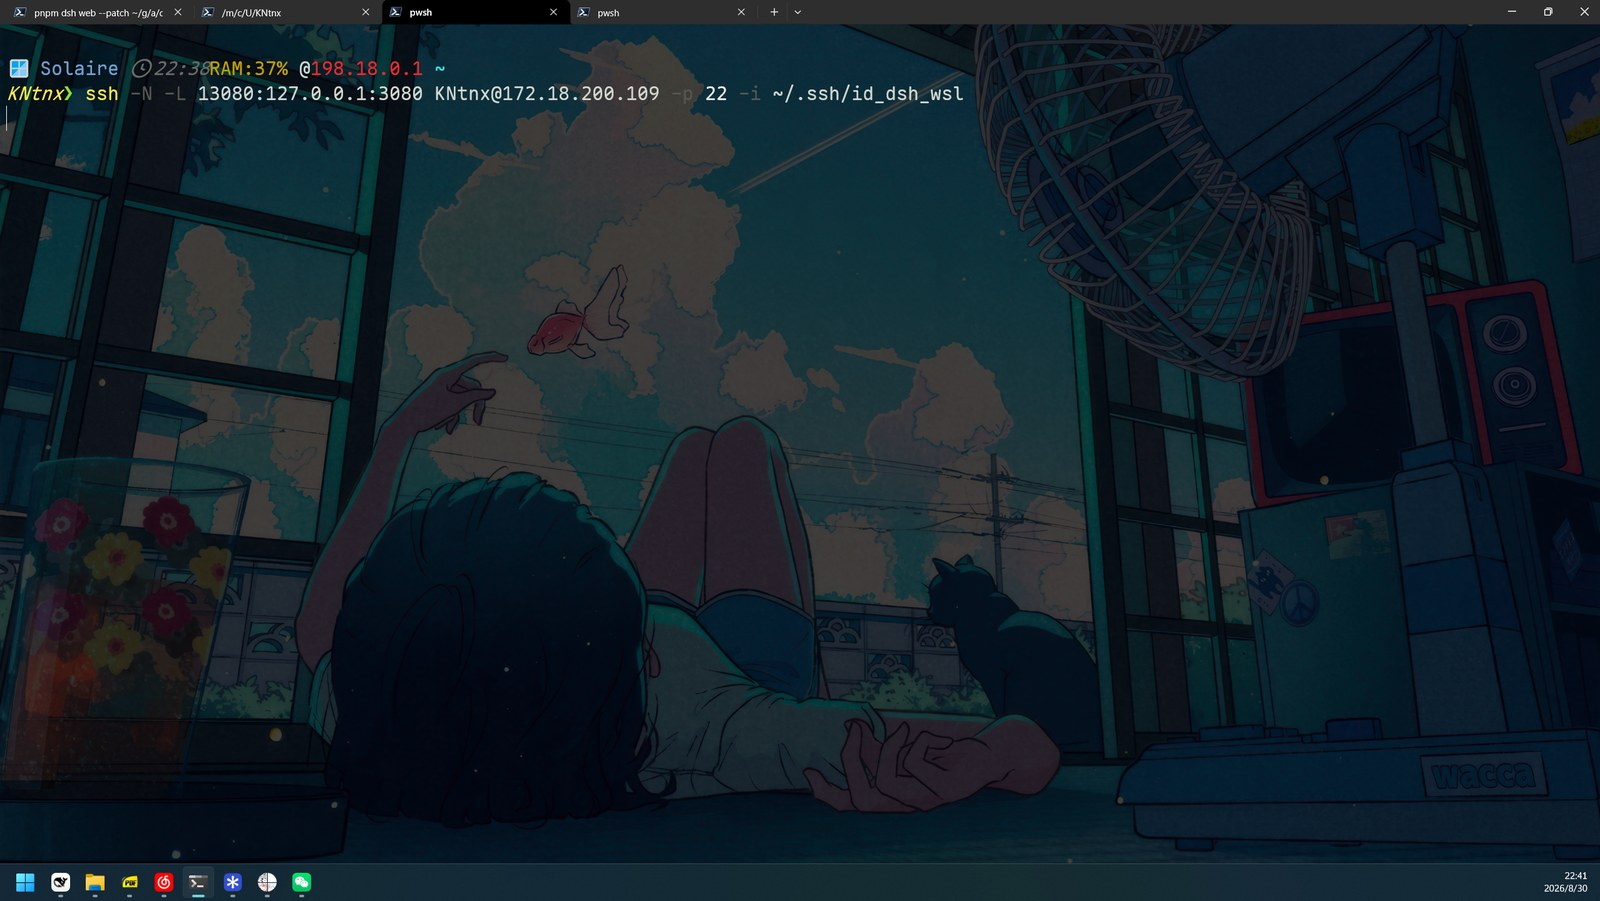
\includegraphics[width=0.62\textwidth]{ch4_ssh_tunnel_cmd.jpg}
\caption{SSH 验证第 2 步：本机建立端口转发——\texttt{ssh -N -L
13080:127.0.0.1:3080 KNtnx@<wsl-ip> -p 22 -i
\textasciitilde/.ssh/id\_dsh\_wsl}（图中 IP 为本机 WSL 虚拟网卡地址，
动态分配）。}
\label{fig:ch4_ssh_tunnel}
\end{figure}

\begin{figure}[H]
\centering
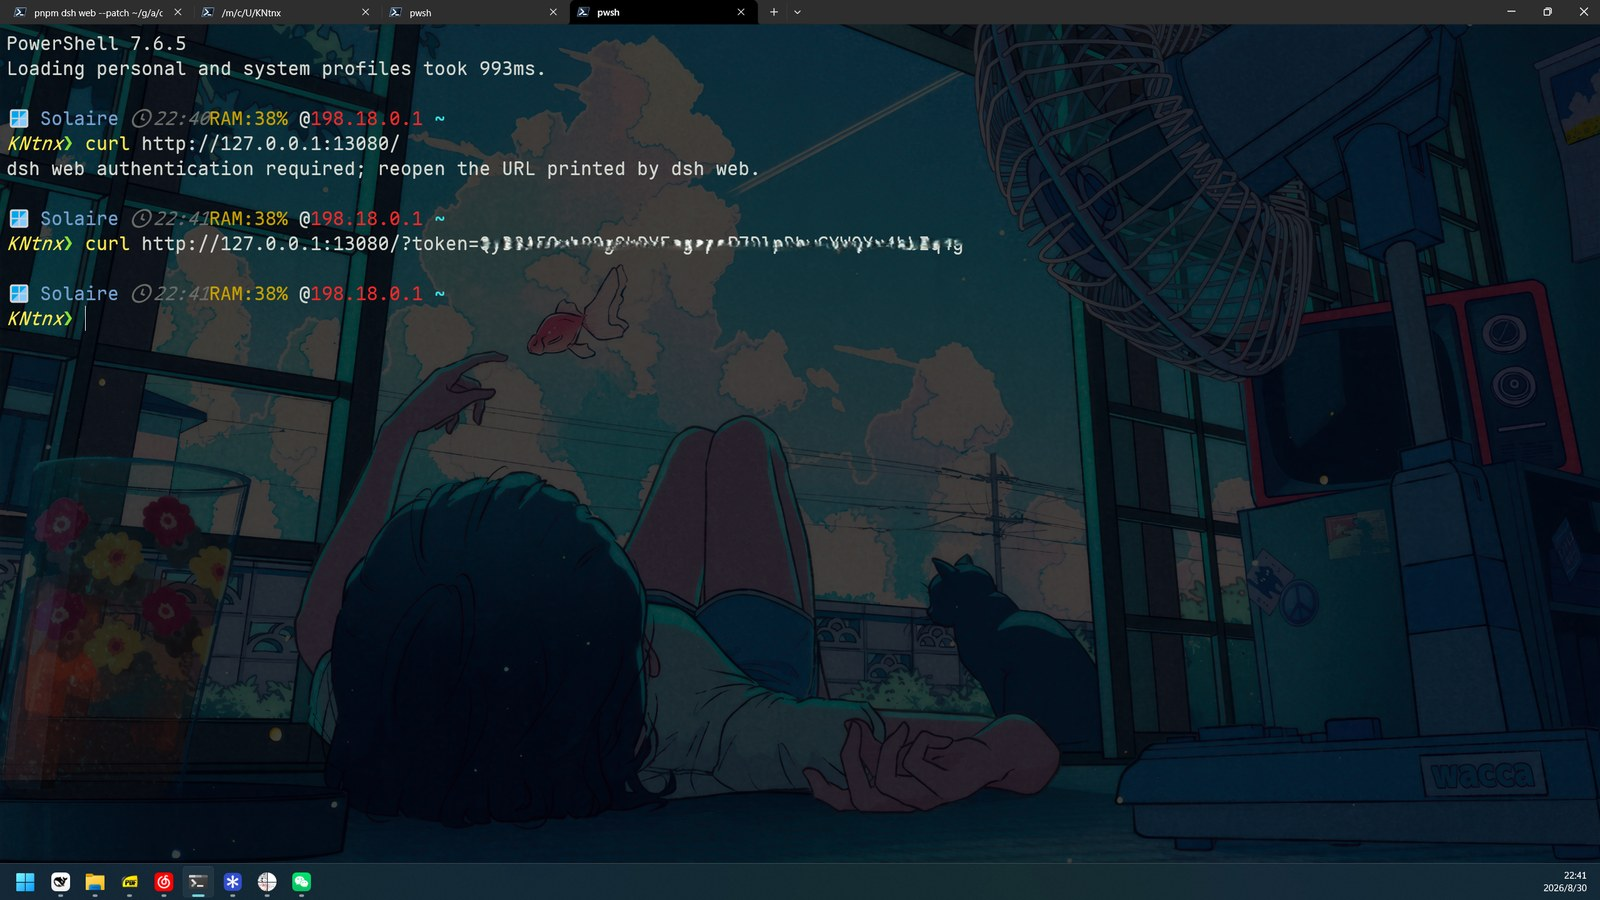
\includegraphics[width=0.68\textwidth]{ch4_ssh_auth_verify.jpg}
\caption{SSH 验证第 3 步：\texttt{curl http://127.0.0.1:13080/} 返回
DSH 令牌鉴权提示（authentication required），随后带
\texttt{?token=...} URL（已打码）访问成功——请求穿透隧道到达远端 DSH。}
\label{fig:ch4_ssh_verify}
\end{figure}

\begin{figure}[H]
\centering
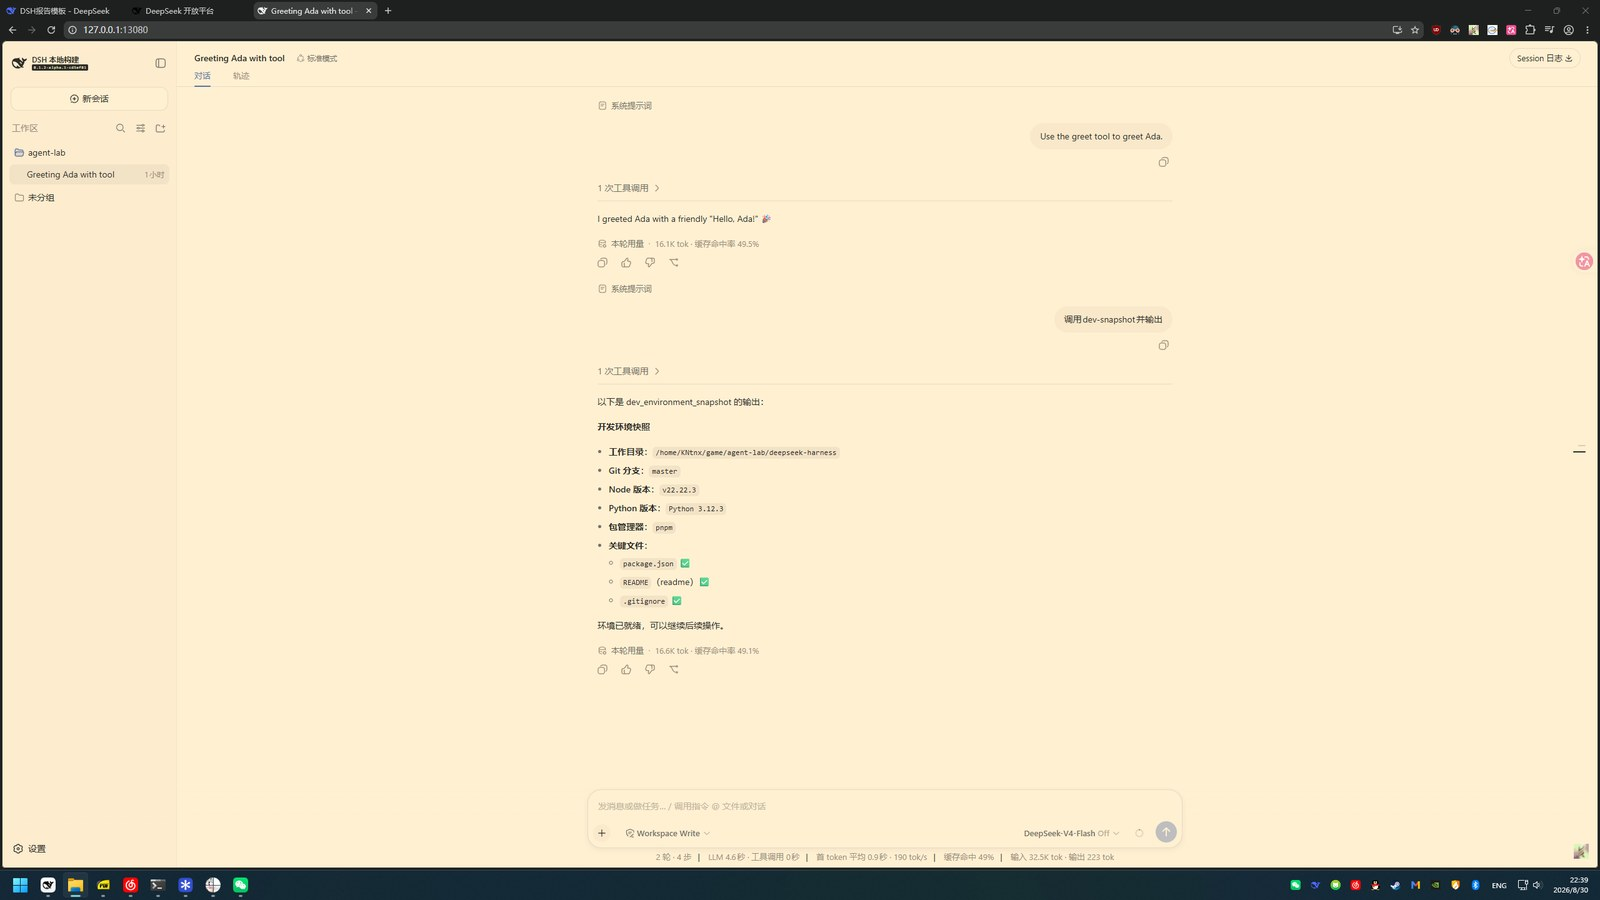
\includegraphics[width=0.88\textwidth]{ch4_remote_ui.jpg}
\caption{通过 SSH 端口转发访问的远端（WSL，独立主机视角）DSH Web UI：
地址栏 \texttt{127.0.0.1:13080}（隧道本地端口），同一会话中 greet 与
dev\_environment\_snapshot 两个工具被模型真实调用并展示结果。}
\label{fig:ch4_remote}
\end{figure}

安全要点（对照任务书第 5 步）：DSH 只监听 \texttt{127.0.0.1}，从网卡
不可达；SSH 转发是唯一访问通道（加密）；公钥认证权限 600/700；
DSH 令牌鉴权为第二道保护；内网 IP 以 \texttt{<wsl-ip>} 占位（动态分配
+ 脱敏，实测值仅保存在本地证据文件）。

模型配置（第 6 步）：DSH 启动时自动把环境中密钥导入
\texttt{DSH\_HOME/.credentials.yaml}（600 权限，Web UI Settings
$\rightarrow$ Models 可见）；密钥只进凭据文件与环境变量，不进入仓库
与报告。

Workspace（第 7 步）：远端项目目录 \texttt{~/game/agent-lab/projects} 与
\texttt{~/game/agent-lab/deepseek-harness} 在 UI ``选择工作区''可选。
完整命令与本次验证记录见
\nolinkurl{evidence/ch4/06_remote_dsh.txt}。

\subsection{问题与改进}

\begin{enumerate}[leftmargin=4em,itemsep=0pt,topsep=2pt]
    \item \textbf{远程环境}：任务书建议远端 Linux + SSH 隧道访问 3080。
          本章已在本机 WSL2（Ubuntu 24.04）上以\textbf{独立远程主机}视角
          完整验证该方案：不依赖 WSL localhost 镜像，隧道目标为 WSL 虚拟
          网卡地址（\texttt{ssh -L 13080:127.0.0.1:3080 KNtnx@<wsl-ip>}，
          本机 3080 已被本地实例占用故映射 13080），直连登录成功、隧道
          端到端到达 DSH（返回鉴权 401 响应即穿透证明），完整命令与
          验证见 4.4.5 节与 \nolinkurl{evidence/ch4/06_remote_dsh.txt}。
          端口 13080 与任务书示意的 3080 仅为本地端口号调整。
          注：真正的多用户远端场景（每学生一个 DSH\_HOME）未实测。
    \item \textbf{沙箱限制}：DSH 沙箱会拦截子进程窗口与部分 spawn/管道
          操作（vitest 的 fork 池因此不可用），测试改用
          \texttt{node --test --test-isolation=none} 单进程模式；
          curl 的 TLS 凭据访问在沙箱内受限（见第 1 章环境限制说明）。
    \item \textbf{版本漂移}：DSH 处于 developer preview，文档与 API 快速
          迭代。本章命令与版本均记录在案：早期 \texttt{npx} 形态
          \texttt{@deepseek-ai/dsh@0.1.0-rc.6}（npm，实际解析安装为
          CLI 0.1.0-rc.7 / 组件 0.1.0-rc.8，cordis 4.0.1）；本章主环境
          为\textbf{源码编译}（git clone，release
          \texttt{0.1.2-alpha.1}，commit \texttt{cd5ef81}）——两种形态
          版本不同，恰好验证了"记录版本、不把当前行为写成永久事实"的
          必要性（任务书要求）。
    \item \textbf{后续方向}：把 \texttt{dev\_environment\_snapshot} 扩展为
          更完整的研发环境巡检（第 5 章 \texttt{devops-scout} 插件即为
          强化版：增加依赖解析、测试探测、变更安全审计）；插件继续增加
          配置项（settings 服务）与 UI 卡片（\texttt{presentCall/
          presentResult}）接入 DSH Web。
\end{enumerate}

\begin{thebibliography}{9}

\bibitem{dsh-repo}
DeepSeek. DeepSeek Harness GitHub 仓库[EB/OL].
\url{https://github.com/deepseek-ai/DeepSeek-Harness}，访问日期 2026-08-18.

\bibitem{dsh-first}
DeepSeek. Your first plugin——DSH 官方插件教程[EB/OL].
\url{https://github.com/deepseek-ai/DeepSeek-Harness/blob/master/docs/user/develop/basic/index.md}，访问日期 2026-08-18.

\bibitem{dsh-tool}
DeepSeek. Build a tool——DSH 官方工具教程[EB/OL].
\url{https://github.com/deepseek-ai/DeepSeek-Harness/blob/master/docs/user/develop/basic/tool.md}，访问日期 2026-08-18.

\bibitem{dsh-publish}
DeepSeek. Package and install a plugin——DSH 官方发布教程[EB/OL].
\url{https://github.com/deepseek-ai/DeepSeek-Harness/blob/master/docs/user/develop/basic/publish.md}，访问日期 2026-08-18.

\bibitem{dsh-cookbook}
DeepSeek. Tool authoring reference——DSH 工具契约参考[EB/OL].
\url{https://github.com/deepseek-ai/DeepSeek-Harness/blob/master/docs/cookbook/adding-a-tool.md}，访问日期 2026-08-18.

\bibitem{dsh-arch}
DeepSeek. DSH Architecture[EB/OL].
\url{https://github.com/deepseek-ai/DeepSeek-Harness/blob/master/docs/architecture.md}，访问日期 2026-08-18.

\bibitem{openssh}
OpenSSH. Port forwarding manual[EB/OL].
\url{https://www.openssh.com/manual.html}，访问日期 2026-08-18.

\bibitem{dsh-video}
Bilibili. 【极速入门】DeepSeek Harness 上手实战指南[EB/OL].
\url{https://www.bilibili.com/}，访问日期 2026-08-18.
（视频资料仅作辅助；本章关键命令与事实均以官方文档与源码为准，未采用
视频内容作为依据——任务书允许视频仅作辅助。）

\end{thebibliography}

% ============================================================
%  第五章（选作）：用 DSH 实现个人 Alpha —— 项目学习报告助手
%  （dsh-learning-report）
% ============================================================
\clearpage
\section{第五章（选作）：用 DSH 实现个人 Alpha —— 项目学习报告助手}

\subsection{背景：问题定义}

\textbf{一句话问题定义}：学习或接手一个陌生项目时，需要回答``它是什么、
怎么搭、怎么跑''——依赖清单、文档入口、目录结构、git 状态、构建命令，
人工要逐文件探测、逐个命令试跑，费时且容易漏。本 Alpha 把它做成一个
DSH 插件（\nolinkurl{code/ch5-alpha/dsh-plugins/} 仓库中的
\texttt{dsh-learning-report}）：用户一句话（``分析这个项目，写技术报告
和复现方案''），模型按插件分发的 skill 工作流自动完成——一次收集结构化
项目快照，产出 \texttt{TECHNICAL\_REPORT.md}（技术报告）与
\texttt{REPRODUCTION.md}（复现方案），全部落盘为文件。

插件已安装进\textbf{Windows 11 本机 DSH 的 desktop profile}
（\texttt{DSH\_HOME=C:\textbackslash Users\textbackslash KNtnx\textbackslash .dsh}）。

\subsection{实验目标}

\begin{enumerate}[leftmargin=4em,itemsep=0pt,topsep=2pt]
    \item 以 bundle 形式把插件装入本机 desktop profile，并验证
          \textbf{真实启动加载}（终端打印插件已加载）；
    \item 梳理插件的工具/skill 结构与数据来源（文件系统与 git），
          画出最小架构；
    \item 落实安全边界：只读收集、输出目录限定、敏感文件不读内容、
          人工确认；
    \item 记录一次真实输入输出（运行证据，见 5.4）。
\end{enumerate}

\subsection{步骤与环境}

环境：Windows 11（DSH\_HOME \texttt{C:\textbackslash Users\textbackslash KNtnx\textbackslash .dsh}，
desktop profile 为 web-app 形态）；DSH 0.1.0-rc.6（npm 全局）；插件
$@$0.1.0（本地 bundle）。插件仓库
\nolinkurl{code/ch5-alpha/dsh-plugins/}（pnpm workspaces；本 Alpha
采用项目报告插件 \texttt{dsh-learning-report}，其余包不在本 Alpha
范围）。安装方式与第 4 章相同（官方 bundle 流程：
\texttt{dsh plugin --profile desktop add <包 tgz>}），插件包内含
\texttt{src/learning-report.ts}（\texttt{collect\_project\_context}）、
\texttt{skills/learning-report/}（项目报告五阶段工作流）与
\texttt{lib/}、\texttt{cordis.patch.yml}。\textbf{真实加载证据}见图~\ref{fig:ch5_loaded}
（首次以默认端口启动时 \texttt{EADDRINUSE: 3080}，按提示改用
\texttt{--port 3081} 后加载成功——排错过程一并保留展示）：

\begin{figure}[H]
\centering
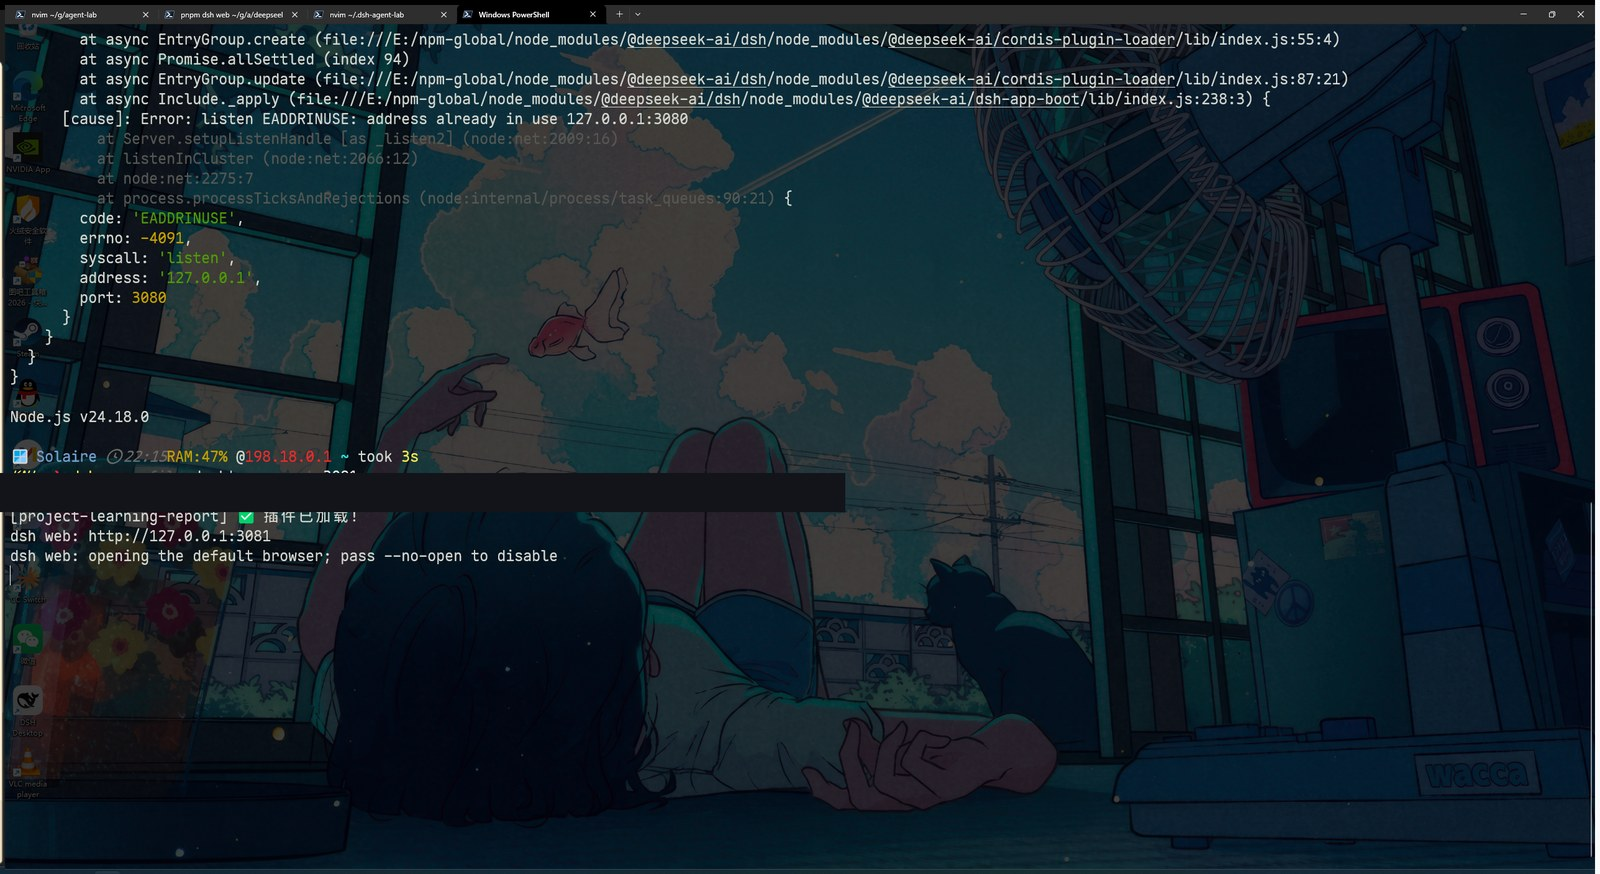
\includegraphics[width=0.95\textwidth]{ch5_plugin_loaded.jpg}
\caption{desktop profile 真实启动：\texttt{dsh --profile desktop
--port 3081} 后终端打印 \texttt{[project-learning-report] 插件已加载！}
（上方为端口占用排错记录；图中另有一行插件加载输出已按本章范围遮盖）。}
\label{fig:ch5_loaded}
\end{figure}

\subsection{结果：真实运行证据}

对真实项目 \textbf{HighWayFlow}（强化学习高速赛车 Gymnasium 环境项目，
位于 \texttt{E:\textbackslash game\textbackslash learn-llm}）执行一次
``写技术报告和复现方案''（图~\ref{fig:ch5_session}）：会话中加载
\texttt{project-learning-report} skill，
\texttt{collect\_project\_context} 首次调用完成结构化快照收集，
随后模型按工作流补读关键文件并落盘两份报告——会话统计共
\textbf{18 次工具调用}（1 次 \texttt{collect\_project\_context} +
补读/写盘等内置工具调用），随后汇报交付文件：

\begin{figure}[H]
\centering
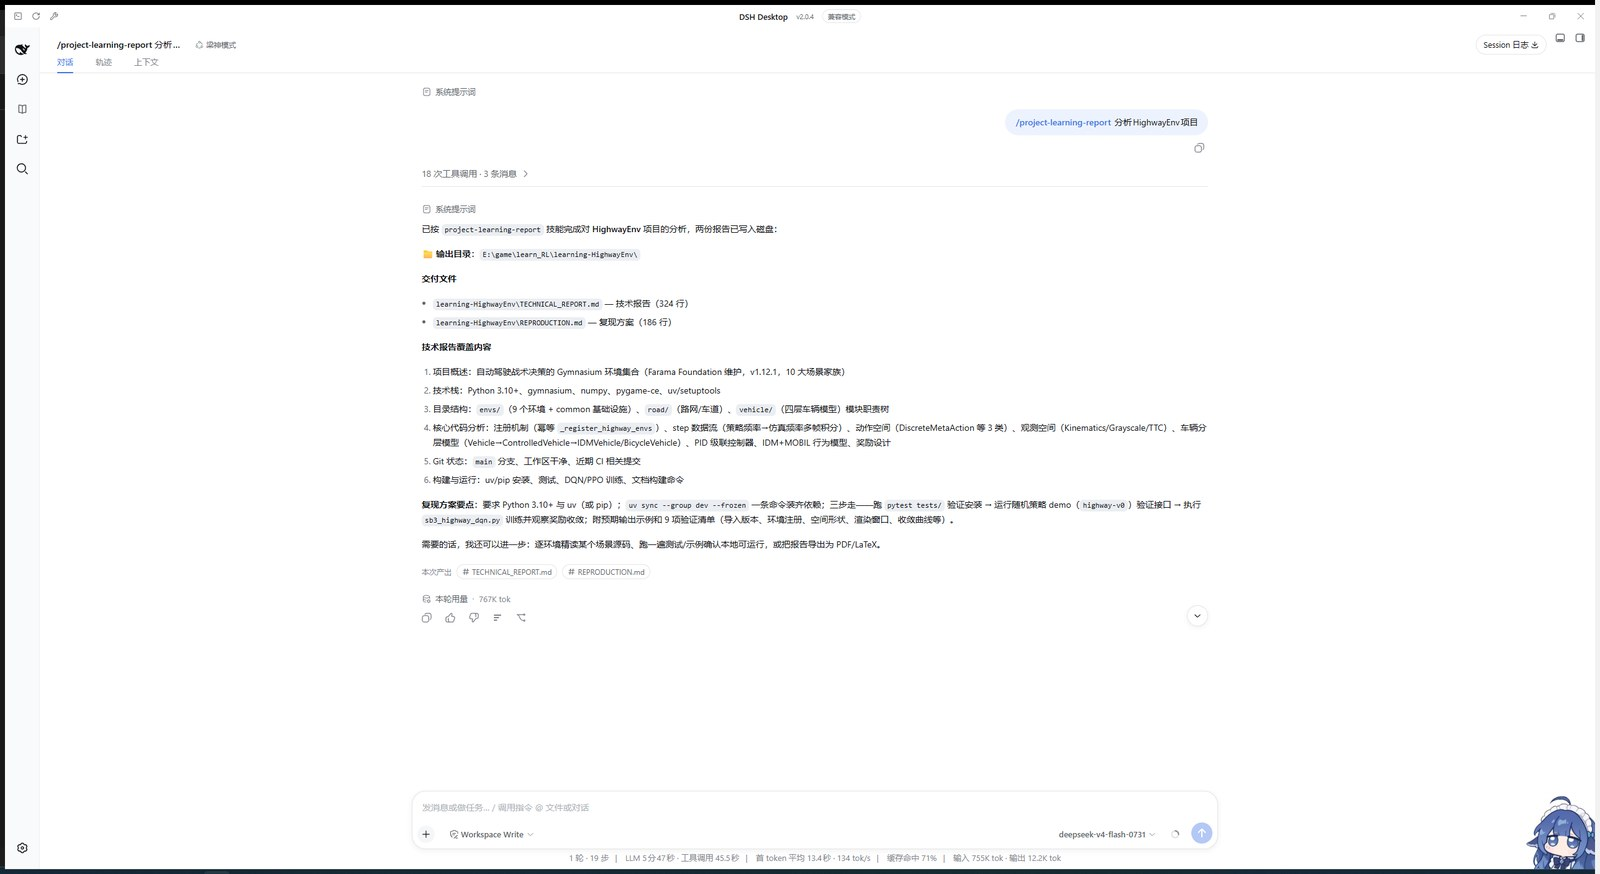
\includegraphics[width=0.95\textwidth]{ch5_session_result.jpg}
\caption{运行结果（desktop 会话）：\texttt{project-learning-report
分析 HighWayFlow 项目}——会话共 18 次工具调用，输出目录
\texttt{E:\textbackslash game\textbackslash learn-llm\textbackslash
learning-highwayflow}，交付 \texttt{TECHNICAL\_REPORT.md}（328 行）与
\texttt{REPRODUCTION.md}（156 行），并给出技术报告与复现方案要点摘要。}
\label{fig:ch5_session}
\end{figure}

\subsubsection{交付文件 1：TECHNICAL\_REPORT.md}

按 SKILL 固定结构成文（项目概述/技术栈与依赖/目录结构/核心代码分析/
Git 状态/构建与运行），图~\ref{fig:ch5_tech} 为其中依赖与目录结构段
（依赖清单精确到版本与用途，目录树带中文批注——例如
\texttt{highwayflow/envs/vehicle/} 下 \texttt{kinematics.py}（车辆运动学）
与 \texttt{controller.py}（纵向/横向 PID 控制器））：

\begin{figure}[H]
\centering
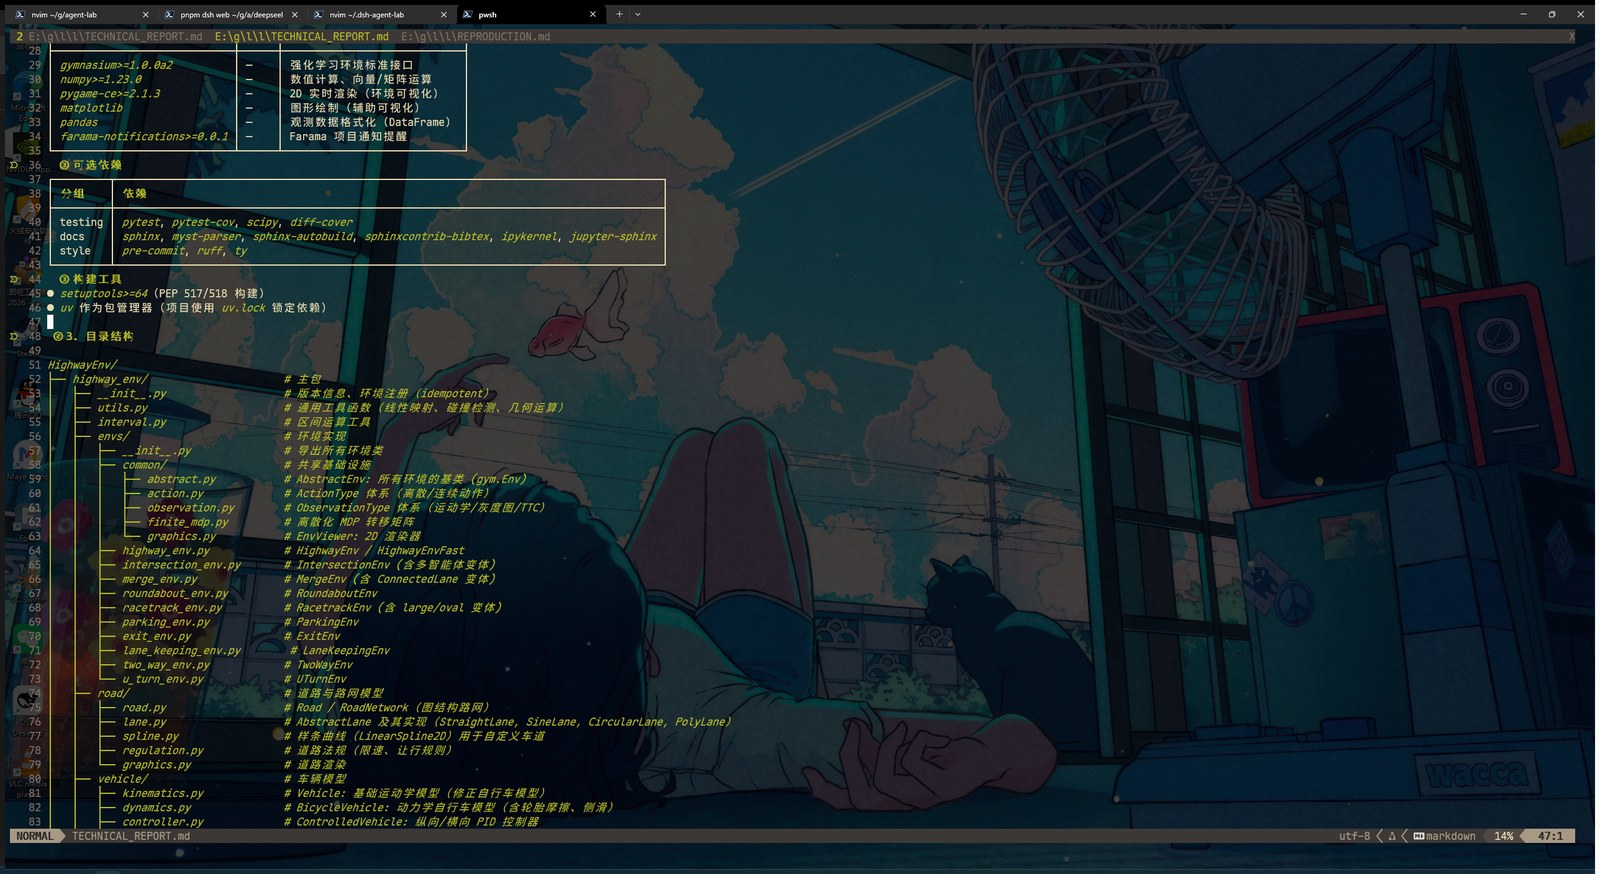
\includegraphics[width=0.95\textwidth]{ch5_report_technical.jpg}
\caption{TECHNICAL\_REPORT.md（编辑器打开）：第 3 段 依赖与工具（gymnasium
0.31.0、numpy、pandas 等；testing/style 工具表；uv 作为包管理器）与
第 4 段 目录结构（带中文模块批注）——高亮行为截图中的表格例。}
\label{fig:ch5_tech}
\end{figure}

\subsubsection{交付文件 2：REPRODUCTION.md}

按 SKILL 固定结构成文（环境要求/依赖安装/复现步骤/预期结果/验证清单），
图~\ref{fig:ch5_repro} 为第 4 段复现结果与第 5 段验证清单（42 个测试 12.3s 全部
通过；验证清单逐项给出验证方法——如
\texttt{python -c "import highway\_env"} 预期输出 \texttt{1.22.1}——
与预期结果列一一对应）：

\begin{figure}[H]
\centering
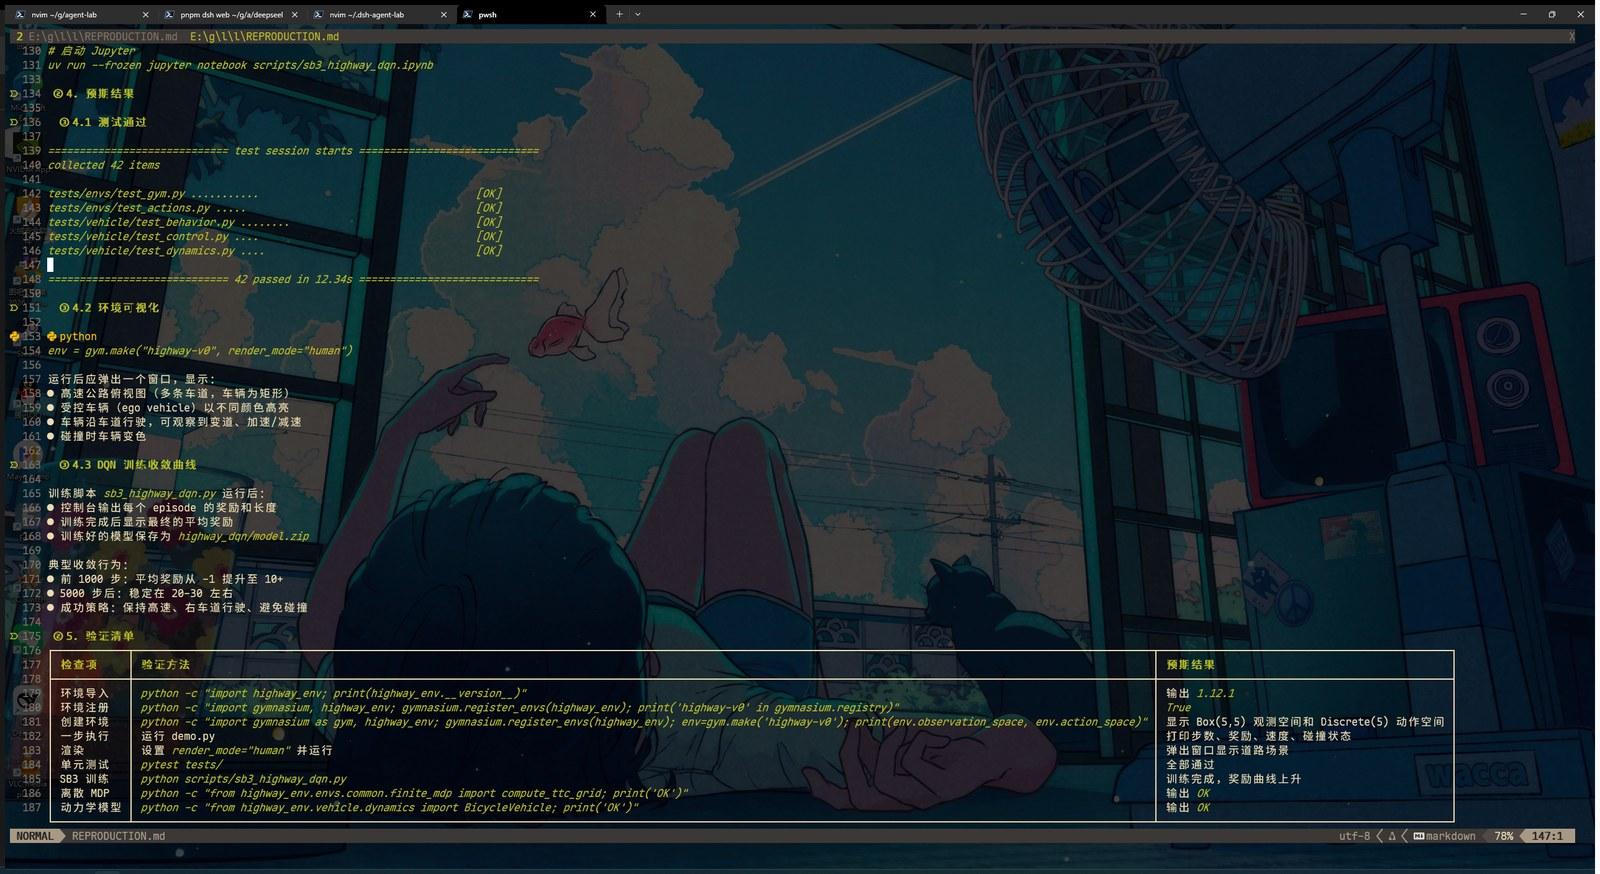
\includegraphics[width=0.95\textwidth]{ch5_report_reproduction.jpg}
\caption{REPRODUCTION.md（编辑器打开）：第 4 段 复现结果（42 tests passed
in 12.3s、环境可视化、DQN 训练曲线）与第 5 段 验证清单（检查项/验证方法/
预期结果三列）。}
\label{fig:ch5_repro}
\end{figure}

至此完成``一句话 → 结构化快照 → 技术报告 + 复现方案''的完整闭环：
\texttt{collect\_project\_context} 一次调用拿到
manifest/README/AGENTS.md/文件清单/git 状态（省 token），模型仅补读
少数关键文件；两份报告全部落盘为文件（不在对话里贴长文）。

\subsection{分析与反思}

\textbf{最小架构}见图~\ref{fig:ch5_arch}（按已安装 bundle 的
\texttt{cordis.patch.yml}、工具声明与 SKILL.md 绘制）：用户一句话 →
skill 工作流阶段化驱动（阶段 1--5）→ 插件工具
\texttt{collect\_project\_context}（一次拿到结构化快照，省 token）与
宿主内置工具（read/write/grep/bash 补读与落盘）→ 数据/产物两路：
项目仓库（清单/文档/源码/git）$\Rightarrow$ 产物
\texttt{learning-<项目>/} 下两个 Markdown。skill 层负责``怎么编排''，
工具层负责``能做什么''，分离使工具可被其它工作流复用。

\begin{figure}[H]
\centering
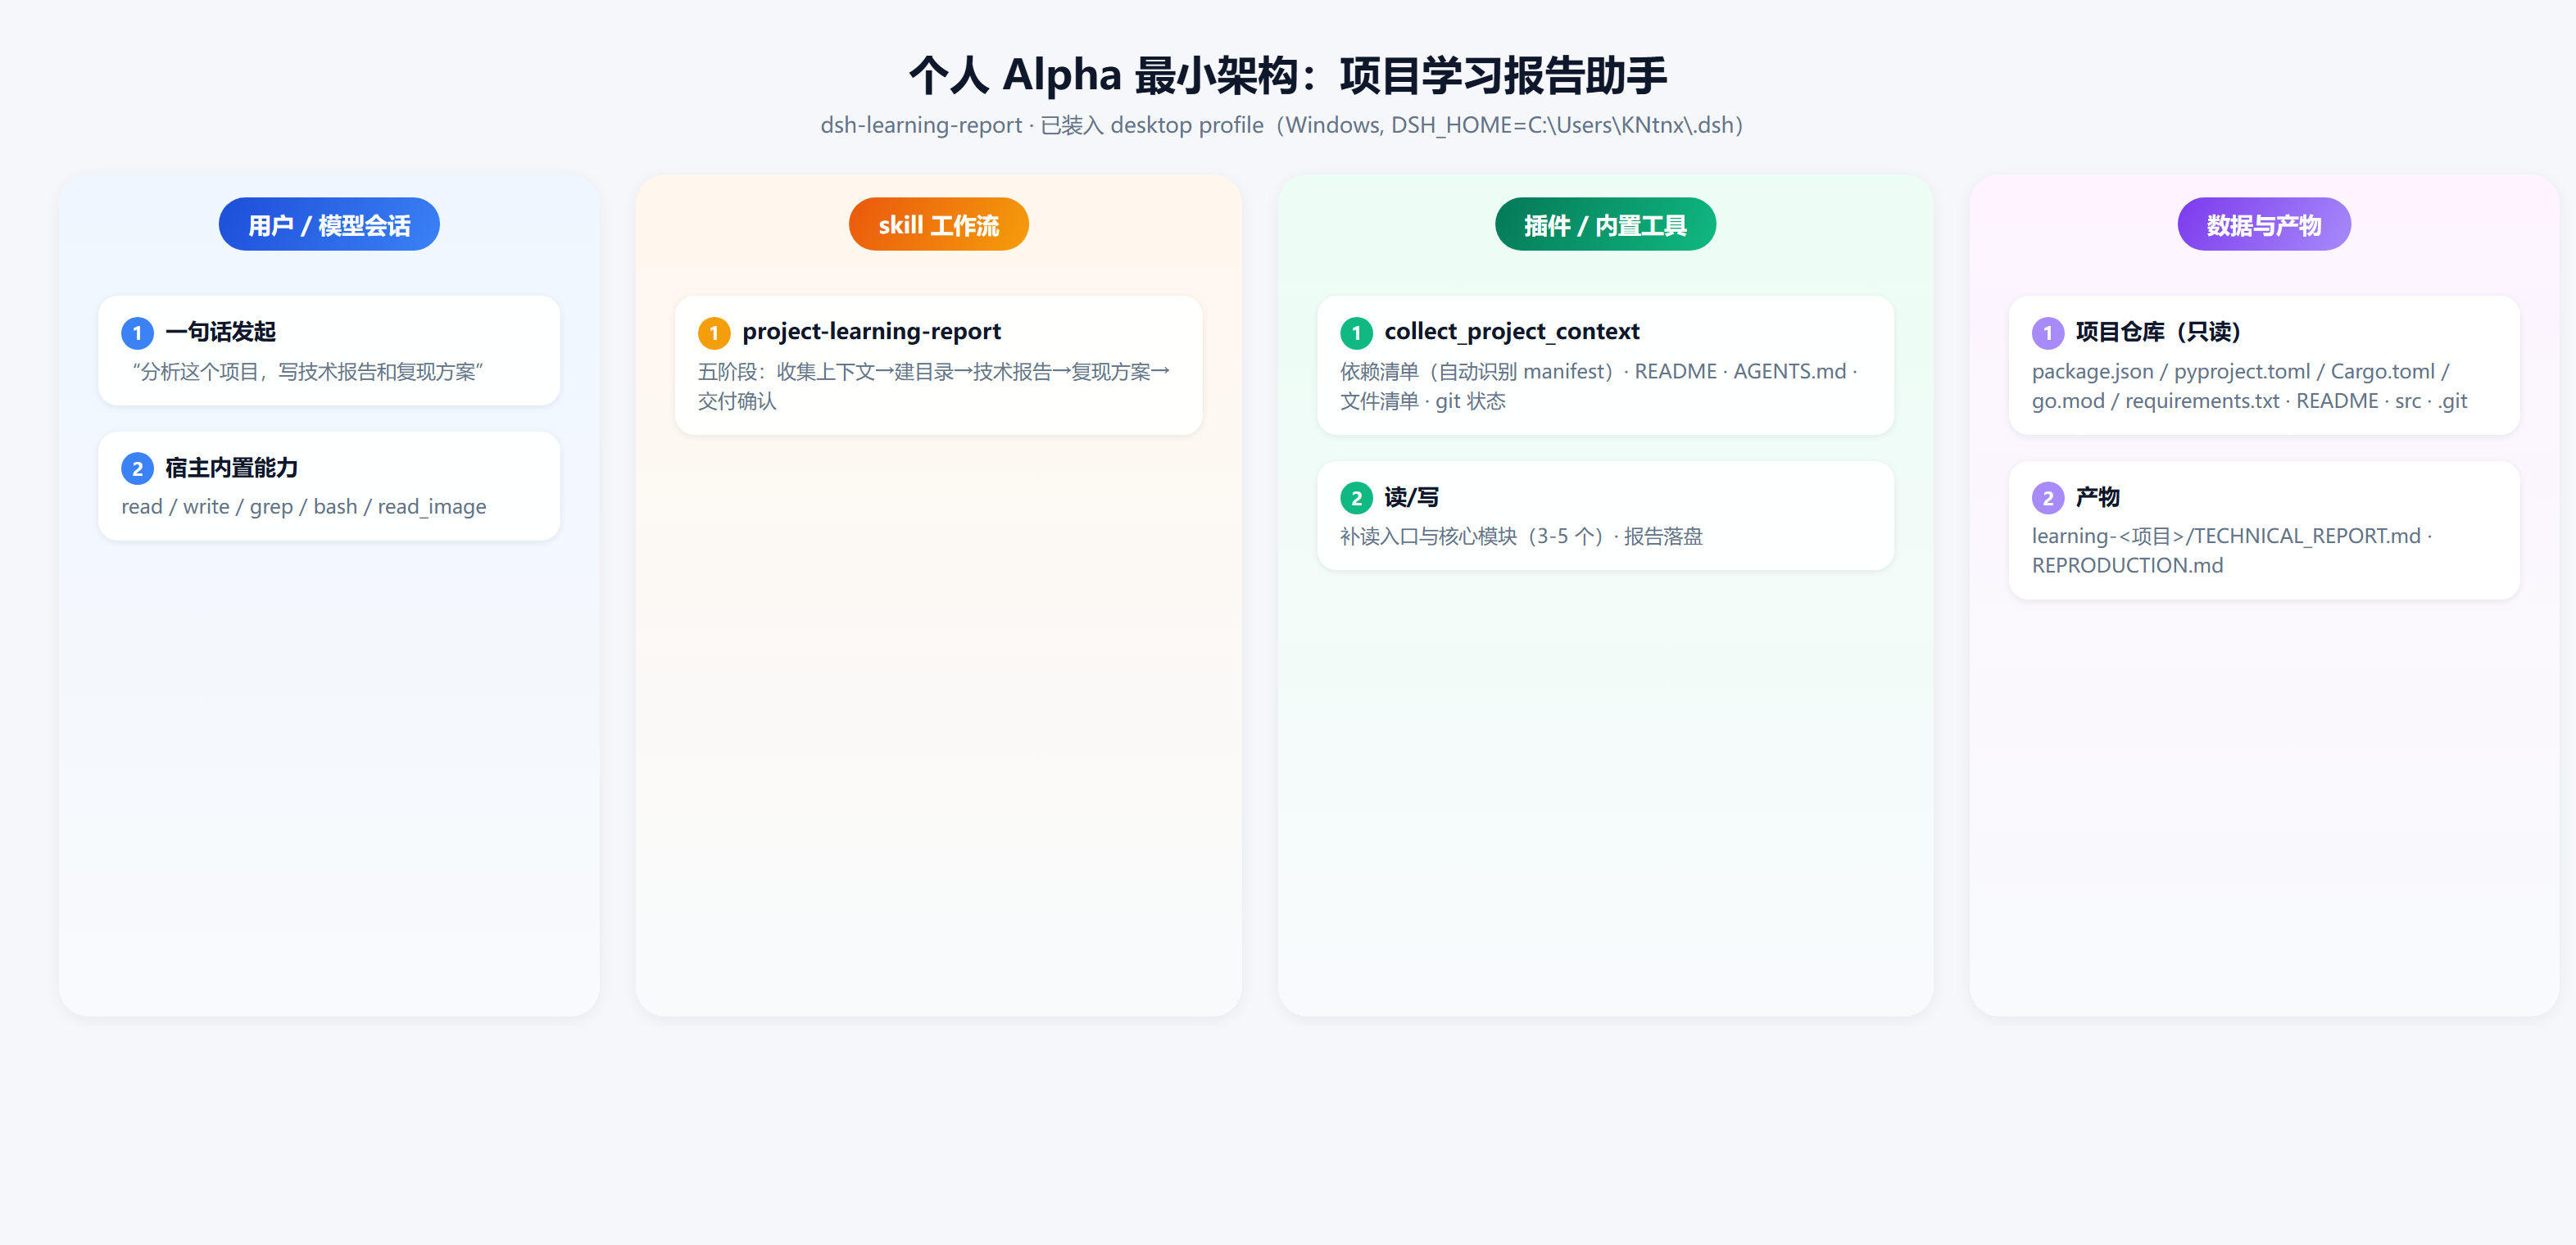
\includegraphics[width=0.95\textwidth]{ch5_arch.png}
\caption{个人 Alpha 最小架构：用户/会话、skill 工作流、插件工具与
数据/产物四层；\texttt{collect\_project\_context} 与
\texttt{project-learning-report} 均来自已安装的 bundle。}
\label{fig:ch5_arch}
\end{figure}

\textbf{为什么适合用 DSH/插件化实现}：``一次收集 + 组织 + 落盘''是
\textbf{多工具、可组合、带权限边界}的职责——DSH 插件模型统一了参数校验
（\texttt{defineTool}）、输出 schema（供程序消费）与权限边界；skill
把收集-写作流程固化为不可变的会话行为，避免每次重复交代；bundle 可被
任意 profile 复用（已验证 desktop 形态加载）。

\textbf{安全边界}：
\begin{enumerate}[leftmargin=4em,itemsep=0pt,topsep=2pt]
    \item \textbf{只读收集}：\texttt{collect\_project\_context} 只读
          项目清单/文档/文件列表/git 状态（git 命令为只读形态），
          写操作限定在产物目录 \texttt{learning-<项目>/}；
    \item \textbf{敏感文件}：不读取 \texttt{.env} 等凭据文件（快照只含
          清单与文件名，不含文件内容密钥）；产物不含 API key；
    \item \textbf{不覆盖}：输出目录已存在时不覆盖已有报告，文件冲突
          采用追加或另命名（SKILL 规定）；\texttt{collect\_project\_context}
          返回的清单用于快照而非逐份粘贴全文（省 token 且保证
          上下文可控）；
    \item \textbf{人工确认}：报告/复现方案为模型生成的一手产出，
          交付前提示用户核对关键命令与预期结果。
\end{enumerate}

\textbf{局限性}与下一步：
\begin{enumerate}[leftmargin=4em,itemsep=0pt,topsep=2pt]
    \item 快照质量依赖源项目结构：manifest 识别覆盖 package.json、
          pyproject.toml、Cargo.toml、go.mod、requirements.txt，
          老式或混合项目可能识别不全；
    \item \texttt{git} 依赖本机 CLI（与第 4 章相同的环境前置）；
    \item 下一步：接入 DSH \texttt{tools/pre-execute} 做产出前检查；
          支持批量/定时学习任务；报告模板参数化。
\end{enumerate}

\begin{thebibliography}{9}

\bibitem{dsh-plugins-ch5}
本项目. dsh-plugins——个人插件仓库（项目学习报告插件）[EB/OL].
\nolinkurl{code/ch5-alpha/dsh-plugins/}，访问日期 2026-08-31.

\bibitem{dsh-skill-ch5}
DeepSeek. DSH 技能（skills）与插件开发文档[EB/OL].
\url{https://github.com/deepseek-ai/DeepSeek-Harness/tree/master/docs}，
访问日期 2026-08-31.

\end{thebibliography}

% ============================================================
%  附录：代码仓库地址、环境版本总表、参考资料总表、截图脱敏声明
% ============================================================
\clearpage
\appendix
\section{附录}

\subsection{代码仓库地址}

\begin{itemize}[leftmargin=4em,itemsep=0pt,topsep=2pt]
    \item \textbf{实训工作区（完整仓库}：实验脚本、证据、报告源码、
          插件源码，\texttt{E:\textbackslash game\textbackslash 2026下半年暑假实训}；
          本地 git 仓库（\texttt{git init} 于 2026-08-19，随章节推进持续
          提交，提交信息见仓库历史）；\texttt{.env} 已被 \texttt{.gitignore}
          排除，不会随仓库外传。GitHub链接：https://github.com/KNtnx/learn-dsh。
    \item \textbf{干净交付文件夹}（本报告 + 任务书 + 报告用到的源码/证据/
          截图，无中间产物）：\texttt{E:\textbackslash game\textbackslash
          2026下半年暑假实训\textbackslash 2026智能23-1bf陈昊\&胡宇星组}。
    \item \textbf{个人插件仓库}（第 5 章 \texttt{dsh-learning-report} 等）：
          \nolinkurl{code/ch5-alpha/dsh-plugins/}（含于工作区仓库）。
    \item 第 3 章分析对象：\nolinkurl{github.com/earendil-works/pi}
          （commit \texttt{59a71b2}）。
    \item 第 4/5 章插件参考：\nolinkurl{github.com/omdsh-dev/dsh-toolkit}、
          \nolinkurl{github.com/omdsh-dev/dsh-tool-time} 等（见各章参考文献）。
\end{itemize}

\subsection{环境版本总表}

\begin{table}[H]
\centering
\caption{全报告运行环境与依赖版本总表}
\label{tab:appendix_env}
\small
\setlength{\tabcolsep}{4pt}
\begin{tabular}{lp{8.2cm}}
\toprule
\textbf{项目} & \textbf{版本/配置} \\
\midrule
操作系统 & Windows 11 专业版（build 26200 / 25H2） \\
Python & 3.11.15（Miniconda 环境 ML-base，E:\textbackslash{}Miniconda\textbackslash{}envs\textbackslash{}ML-base） \\
openai SDK & 2.37.0（第 1/2 章实验；.env 解析为脚本内置实现，无需额外依赖） \\
matplotlib & 3.10.9（图表绘制） \\
Node.js / npm / pnpm & v24.18.0 / 12.0.2 / 11.22.0 \\
DSH & @deepseek-ai/dsh 0.1.0-rc.6（npm 全局） \\
@deepseek-ai/dsh-tools / cordis & 0.1.0-rc.6 / 4.0.1 \\
git / curl & 2.55.0.windows.4 / 8.21.0 \\
TeX Live & 2025（xelatex / latexmk / ctex / gbt7714） \\
Pi（第 3 章） & @earendil-works/pi-agent-core 0.84.2（commit 59a71b2） \\
模型 & mimo-v2.5（第 1/2 章主实验）；kimi-k3（第 1 章模型对比实验） \\
\bottomrule
\end{tabular}
\end{table}

\subsection{参考资料总表}

各章参考文献已列于章末。此处汇总全部引用类型：国内模型官方 API 文档
（Kimi/小米 MiMo/火山方舟/阿里云百炼/DeepSeek）、HTTP/JSON/curl 基础资料
（MDN/RFC 8259/curl 官方）、prompt/context/agent 论文与深度文章（ReAct、
Anthropic 系列、OpenAI harness engineering）、Pi 与 DSH 源码与官方文档、
远程开发资料（OpenSSH）以及社区插件仓库。所有引用均注明标题、URL 与
访问日期（2026-08-17 至 2026-08-19）。

\subsection{截图脱敏声明}

\begin{enumerate}[leftmargin=4em,itemsep=0pt,topsep=2pt]
    \item 第 1 章全部运行窗口截图与控制台截图经逐张检查：无 API key 明文
          （平台以星号/部分字符遮挡，或由作者手动遮挡）；
    \item DeepSeek 控制台截图中的充值余额已由作者遮挡；累计消费为账户历史
          统计，图注已说明；
    \item 报告全文与仓库中不存在明文密钥；\texttt{.env} 仅存本机并被
          \texttt{.gitignore} 排除；
    \item 第 5 章审计工具输出统一经脱敏层处理（sk- 等模式替换为占位符）。
\end{enumerate}


\end{document}
